\chapter{Dialektale Deklinationssysteme in den ostoberdeutschen Dialekten Bayerns}
\label{chap:8}
Deklinationsklassen stellen eine abstrakte Klassifikation von Substantiven dar, welche sich dieselben formalen Flexionsmarker im Paradigma teilen (vgl. \chapref{chap:3}.). Für die Einteilung der mhd. oder nhd. Deklinationsklassen werden „mehr oder weniger zwangsläufig“ (\citealt[71]{KleinEtAl2018}) die Kasusexponenten des Genitiv Singular und die Pluralallomorphe herangezogen, da im Singularparadigma der Genitiv am stärksten distinkte Formen und ein vergleichsweise ausdifferenziertes Markerinventar aufweist; im Pluralparadigma ist bereits im Mittelhochdeutschen nur noch das uniforme Nasalsuffix im Dativ erhalten. Infolge des weitgehenden Abbaus der Kasusmarkierung am Substantiv und verschiedener innerparadigmatischer Ausgleichsprozesse (z.\,B. Übernahme des Flexivs der obliquen Kasus in den Nom.Sg.) berücksichtigen synchrone Klassifikationen dialektaler Flexionssysteme in der Regel nur die Pluralallomorphie, da diese als „einzig klares Kriterium“ verbleibe, wie es beispielsweise \citet[41]{White1966} in seiner Grammatik zum mittelbair. Dialekt von Eisenhofen formuliert. In den rezenten Dialekten handelt es sich also vielmehr um „Pluralbildungsklassen“ \citep[170]{Rowley1997} als um Deklinationsklassen, wie sie historisch in den Sprachstufen des Deutschen zu finden waren. Gleichzeitig manifestieren sich Deklinationsklassen auch in den rezenten Dialekten des Untersuchungsgebiets in zwei Ausprägungen:

\begin{itemize}
\item Die historische Klassenzugehörigkeit ist bewahrt, aufgrund dialektspezifischer phonologischer Prozesse hat in den untersuchten Dialekten aber eine Erhöhung des Inventars morphophonologischer Pluralmarker stattgefunden, sodass die rezenten Entsprechungen der Numerusexponenten der historischen Klassen in der arealen Dimension formal variieren.
\item Diachron hat sich Deklinationsklassenwandel vollzogen, und zwar in Form von Deklinationsklassenwechsel oder weil sich -- teilweise dialektraumspezifische -- außerflexivische Konditionierungsfaktoren herausgebildet haben, die wiederum zu Deklinationsklassenwechsel führten.
\end{itemize}

In der folgenden Darstellung werden die synchrone und diachrone Perspektive, die sich an diesen beiden zentralen Befunden ablesen lässt, konsequent beibehalten. Die dialektalen Deklinationsklassen werden im Folgenden zunächst in ihrer synchronen Zusammensetzung (\sectref{sec:8.1}) und anschließend in ihrer diachronen Entwicklung (\sectref{sec:8.2}) behandelt. \sectref{sec:8.3} fokussiert schließlich die Zusammensetzung der Deklinationsklassen und die Rolle außerflexivischer Faktoren, stets unter Berücksichtigung der arealen Dimension.

\section{Synchrones dialektales Deklinationsklassensystem}
\label{sec:8.1}
Die Darstellung der Formenbildung in \chapref{chap:7} hat gezeigt, dass sich das Pluralmarkerinventar in den untersuchten Dialekten infolge verschiedener historischer phonologischer Prozesse (insbesondere im Bereich der stammaffizierenden Verfahren) ausdifferenziert hat, dass damit synchron Heteromorphie zu beobachten ist. Gleichzeitig wird die Markierung der Kasusinformation am Substantiv in der Tendenz abgebaut, wenngleich auch hier -- nämlich im Falle des Dat.Pl. -- eine dialektspezifische Ausdifferenzierung des additiven Markerinventars stattgefunden hat. Der Abbau der Kasusmarkierung am Substantiv hat in den untersuchten Dialekten noch nicht zu einem vollständigen Verlust der Kasusmarkierung am Substantiv geführt, doch vor allem im Singularparadigma findet sich weitgehender Formensynkretismus; eine distinkte Kasusform ist nur bei den Maskulina im Akkusativ/Dativ zumindest teilweise erhalten, bei den Feminina findet sie sich zum Teil im Dat.Sg. (vgl. \sectref{sec:7.2.2}). Ein synchrones Deklinationssystem der oobd. Dialekte basiert aufgrund dieser sprachinternen Entwicklungen vor allem auf der Pluralallomorphie. Hinzu kommt, dass für die untersuchten Dialekte keine konsistenten Daten zur Kasusflexion im Singular vorliegen, sodass auch aus methodischen Gründen primär die Pluralmarkierung herangezogen werden muss. Da, wo es möglich ist (d.\,h. bei Maskulina der historisch schwachen Deklination, wo Singular-Kasusformen systematisch abgefragt wurden), werden auch Aussagen zur Kasusexponenz des Singulars oder zu spezifischen Paradigmenkonstellationen getroffen. Ausgehend von diesen Überlegungen und auch mit Blick auf die Definition des Klassifizierungsprinzips Deklinationsklasse (\chapref{chap:3}) ist die zentrale Frage der Klasseneinteilung: Wie ähnlich muss das Flexionsverhalten sein, damit Substantive eine Klasse bilden?

Die Bezeichnung der rezenten dialektalen Deklinationsklassen orientiert sich an den formalen Ausprägungen der Klassen (im diachronen Bezug werden allerdings germ. Klassenbezeichnungen verwendet, vgl. \sectref{sec:8.2}). Ich folge darin \citet[27]{Rowley1997} und \citet[124]{Wurzel1984}, die sich jeweils dafür aussprechen, Deklinationsklassen nach den spezifischen Klassenmerkmalen oder -eigenschaften zu benennen. Die Idee des vorgeschlagenen synchronen Deklinationsklassensystems ist es, die Analyse auf mehreren Ebenen zu ermöglichen. Die oberste Ebene bilden Klassentypen, deren Bezeichnung sich an den Pluralmarkierungsverfahren orientiert (\figref{fig:11}): NULL, die additiven (nach den Allomorphen bezeichneten) Klassen N, A, E, R und die stammaffizierende Klasse MOD („modulativ“).\largerpage

Auf dieser Ebene wurde die Differenzierung der additiven Pluralmarker Nasalsuffix, Schwa und Tiefschwa sowie \textit{er}{}-Suffix beibehalten. Diese Lösung wurde gewählt, um die Distribution und Zusammensetzung der verschiedenen additiven Deklinationsklassen dialektübergreifend analysieren zu können. Der methodische Nachteil dieser Form der Klassifikation ist, dass die Heteromorphe \mbox{-\textit{n}}, -\textit{ə} und -\textit{α} als rezente Entsprechungen des Nasalsuffixes (etwa bei \teuthoo{hosn}{hosn}, \teuthoo{hosE}{hosə} oder \teuthoo{hosA}{hosα} ‚Hasen‘) der his\-to\-risch schwachen Maskulina oder die Heteromorphe -\textit{(ə)r}, -\textit{ə} und -\textit{α} als rezente Entsprechung des \textit{er}{}-Suffixes der his\-to\-rischen \textit{iz/az}{}-Klasse (\teuthoo{haisEr}{haisər}, \teuthoo{haisE}{haisə}, \teuthoo{haisA}{haisα} ‚Häuser‘) jeweils unterschiedlichen Klassen zugeordnet werden (siehe \sectref{sec:7.1.1.1} zum Suffixinventar, vgl. \citealt[129]{Rowley1997}). Wo es sinnvoll ist, die Heteromorph-Ebene zu abstrahieren, d.\,h. v.\,a. in der Darstellung des Deklinationsklassenwandels (\sectref{sec:8.2}), wird diese differenzierte Klasseneinteilung zu dialektübergreifenden Klassen zusammengefasst.


\begin{figure}
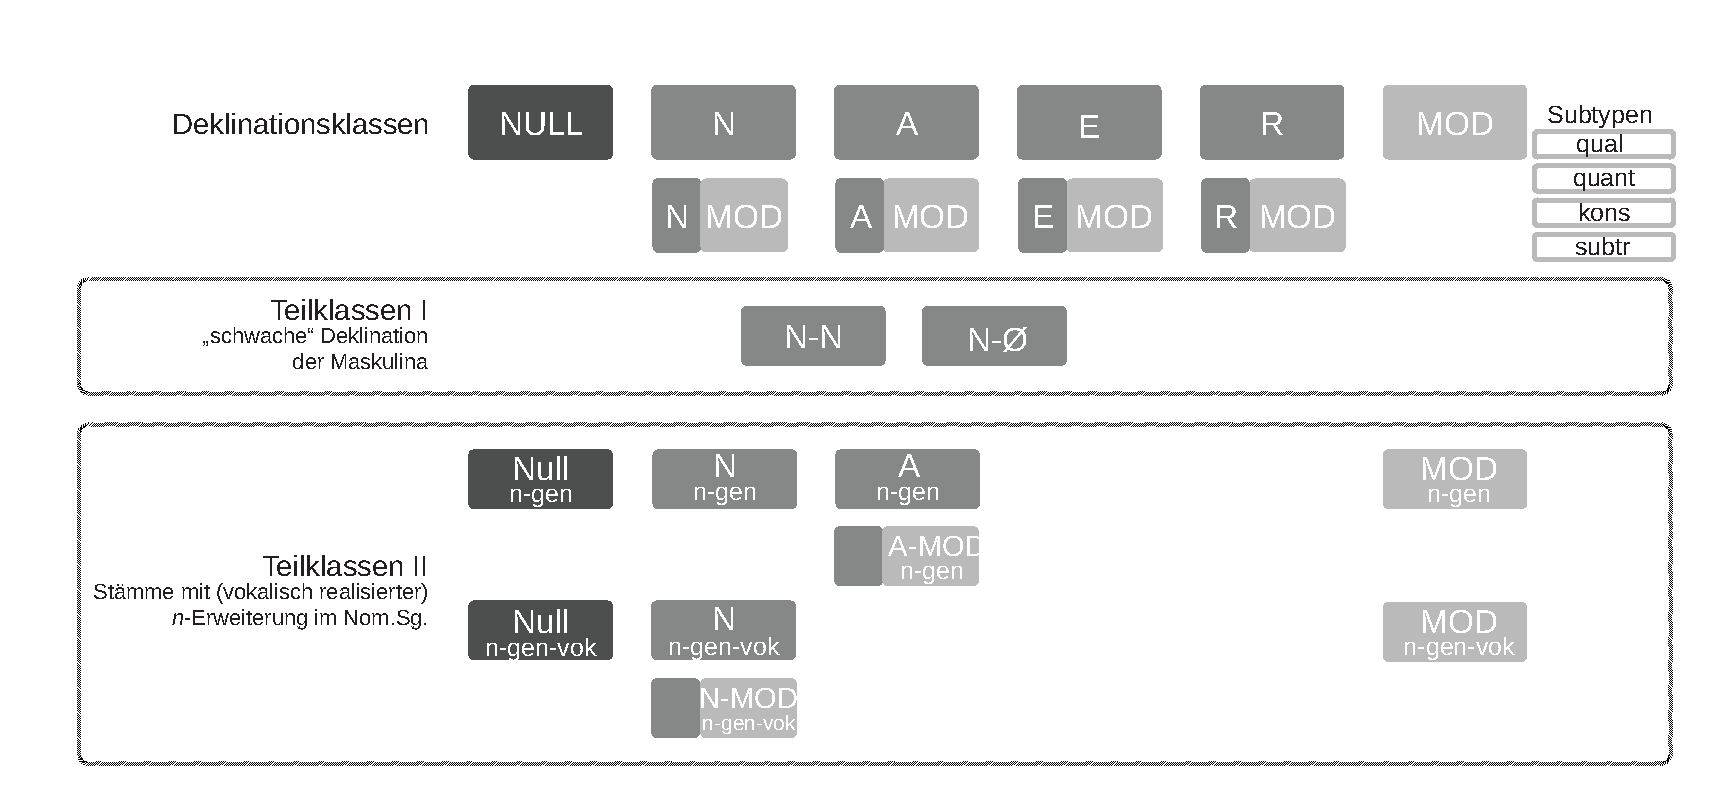
\includegraphics[width=\textwidth]{figures/Deklinationsklassen.pdf}
\caption{Synchrone dialektale Deklinationsklassen}
\label{fig:11}
\end{figure}

Auch in der stammaffizierenden Klasse MOD wird Heteromorphie, d.\,h. dialektspezifische morphophonologische Alternationen, in Form von vier Untertypen berücksichtigt. Die Klasse MOD(qual) umfasst sämtliche Alternationen der Vokalqualität, d.\,h. Umlaut, Wechsel der Zungenhöhe sowie die umlautähnliche Alternation von mhd. \textit{ei}, MOD(quant) bezeichnet Alternationen der Vokalquantität, MOD(kons) sämtliche Alternationen des Konsonantismus (Le"-nis-""For"-tis-""Kon"-tras"-te, 0/K- und K/0-""Al"-ter"-na"-tio"-nen, Spirantisierungen) und MOD"-(subtr) subtraktive Formen. Treten mehrere stammaffizierende Verfahren kombiniert auf, sind diese Subtypen entsprechend annotiert, sodass die Analyse je nach Fragestellung sowohl die übergeordnete Ebene des Klassentyps MOD als auch die konkret realisierten Verfahren der Subtypen berücksichtigen kann, z.\,B. MOD"-(kons, qual, quant) bei \teuthoo{bo.2}{bōͅ} -- \teuthoo{ba4X!}{bạꭖ} ‚Bach‘ (nordbair.-mittelbair. Bernhardswald).

Für die Datenauswertung ist die Idee hinter dieser mehrstufigen Klassenbezeichnung, eine Analyse von einer abstrahierenden Ebene hin zu feineren Abstufungen zu ermöglichen, die einerseits die Kombination von Markierungsverfahren erfasst und zum anderen areal variierende Ausprägungen der einzelnen stammaffizierenden Strategien im Blick hat. Gleichzeitig versucht diese Klassifizierung der mentalen Repräsentation von Flexionsformen nahezukommen. Aus Perspektive einer Dialektgeografie ist es relevant und interessant, welche phonologischen Prozesse historisch zu den morphophonologischen Alternationen bei \teuthoo{kha."+mb\_}{khã̄ͅmbʰ} -- \teuthoo{khe.m}{kheͅm} ‚Kamm‘ (ofr.-hess. Wiesthal), \teuthoo{kha.m}{khaͅm} -- \teuthoo{kha4mb5\_}{khạmb̩ʰ} (nordbair.-mittelbair. Blaibach) oder \teuthoo{k\_a.mbv}{kʰaͅmbv} -- \teuthoo{k\_a4mpf}{kʰạmpf} (mittelbair. Kirchensur) geführt haben. In \sectref{sec:7.1.2} wurde indes gezeigt, dass innerparadigmatische Alternationen, insbesondere jene, die den stammauslautenden Konsonantismus affizieren, his"-to"-ri"-sche phonologische Prozesse konservieren und lexikalisiert sind -- mit der Ausnahme einiger weniger funktionalisierter, produktiver Verfahren wie dem Umlaut. Zudem scheint es aus Sprecherperspektive plausibel, eine einzige Klasse MOD für sämtliche stammaffizierenden Verfahren anzunehmen, und zwar in Abgrenzung von additiven Markierungsverfahren und Null.

Unterhalb der additiven und stammaffizierenden Oberklassen und der kombinierten Klassen (R-MOD, A-MOD, N-MOD, E-MOD) werden zwei Teilklassen beschrieben:

\begin{itemize}
\item In der Denomination der Deklinationsklassen werden Singularstämme, bei denen das Nasalsuffix der obliquen Kasus analog in den Nom.Sg. übertragen wurde, gesondert ausgewiesen, um spezifische Analysen zur Distribution der Pluralallomorphie für diese \textit{n}{}-erweiterten Stämme und ihren relativen Anteil in der Zusammensetzung einzelner Deklinationsklassen zu ermöglichen. Die Denomination der Klassen besteht aus einem Präfix, das das Flexionsverfahren bezeichnet (NULL, N, MOD usw.) und einem Suffix, dass die Realisierung des (historischen) Nasalsuffixes der Singularform angibt: Suffix „n-gen“ für die Realisierung als Nasal, „n-gen-vok“ für die vokalische Realisierung. Als Teilklasse der NULL-Deklinationsklasse erscheint etwa die Klasse NULL-n-gen (Typ \teuthoo{glokN}{ɡlokŋ} -- \teuthoo{glokN}{ɡlokŋ} ‚Glocke‘), als Teilklasse der N-Klasse die Klasse N-n-gen-vok (Typ \teuthoo{biEkA}{biəkα} -- \teuthoo{biEkAn}{biəkαn} ‚Birke‘).
\item Bei historisch schwachen Maskulina, für die systematisch auch oblique Singular-Kasusformen erhoben wurden, wird danach differenziert, ob Kasus eine distinkte Markierung aufweist (Teilklassen N-N) oder synkretische Formen vorliegen (N-∅). Die Denomination der Teilklasse fasst vokalische Realisierungen als Schwa oder Tiefschwa und Realisierungen als Nasalsuffix zusammen.
\end{itemize}

Eine andere grundsätzliche Frage, die sich vor allem für kombinierte Markierungsverfahren stellt, lautet: Welches Flexionsmuster ist klassenkonstituierend, welche Markierungsverfahren werden als konkomitant und damit als nicht klassenkonstituierend analysiert? Im Neuhochdeutschen etwa ist der Umlaut in Kombination mit \textit{er}{}-Suffix (Typ \textit{Huhn} -- \textit{Hühner}) konkomitant, da Umlaut obligatorisch und voll vorhersagbar bei Klassenmitgliedern mit velarem Stammvokal erscheint (vgl. \citealt[69]{Dammel2018} sowie \sectref{sec:4.1}). Hier ist es sinnvoll, eine einzige Deklinationsklasse anzusetzen, die Pluralformen mit \textit{er}{}-Suffix und UL+\textit{er} umfasst.

Für sein nordostbayerisches UG klassifiziert \citet{Rowley1997} kombinierte Markierungen in Form eines additiven und eines stammaffizierenden Markers als Teilklassen einer additiven Deklinationsklasse. So gehörten das Neutrum ofr. \teuthoo{I2sd}{ı̄sd} -- \teuthoo{I2sda}{ı̄sda} ‚Nest‘ und eine Pluralform mit Quantitätskontrast wie ofr. \teuthoo{ne2isd}{nēisd} -- \teuthoo{ne.sde.}{neͅsdeͅ} ‚Nest‘ gleichermaßen zur R-Klasse, das Flexionsmuster mit Quantitätskontrast bildet dabei eine Teilklasse R „mit Dehnung des Singularstamms“ \citep[164]{Rowley1997}. Das stammaffizierende Verfahren ist als „zusätzliche Modifikation“ konkomitant, klassenkonstituierend ist die „besondere Formenkonstellation im Paradigma“: die additive Markierung mit \textit{er}{}-Suffix \citep[145]{Rowley1997}.\footnote{Ähnlich verfährt \citet[41]{White1966}, der zwar Klassen mit vs. ohne Umlautmarkierung differenziert, aber Lenis-Fortis-Kontraste im Stammauslaut als konkomitantes Merkmal ausweist, das phonologisch bedingt ist.} Nur wenn sie ausschließlich vorkommen, konstituieren stammaffizierende Markierungen eine eigene Deklinationsklasse \citep[144]{Rowley1997}. Für eine morphologische Sprachgeografie eignet sich diese Form der Klassifikation \citet[145]{Rowley1997} zufolge, weil im Bereich der stammaffizierenden Verfahren „areal unterschiedliche Kombinationen und regional große Schwankungen beim einzelnen Lexem vorliegen können.“ Nicht unproblematisch ist aber in meinen Augen, dass der additiven Markierung der Status der „besonderen Formenkonstellation“ a priori zugesprochen wird und stammaffizierende Markierungen automatisch konkomitant sind. Hier scheint eine Differenzierung sinnvoll, wie sie \citet[65--66]{Dammel2018} für das Konkomitanzverhältnis von Umlaut und additivem Flexiv im Neuhochdeutschen beschreibt:

\begin{enumerate}[label=(\alph*)]
\item Umlaut wird entweder obligatorisch durch das Flexiv gefordert (z.\,B. beim nhd. \textit{er}{}-Plural, Typ \textit{Huhn} -- \textit{Hühner}) oder er ist durch das Flexiv ausgeschlossen (z.\,B. beim nhd. \textit{(e)n}{}-Plural). Beim \textit{e}{}-Suffix erscheint Umlaut nur bei den Feminina der historischen \textit{i}{}-Deklination (Typ \textit{Kraft} -- \textit{Kräfte}) automatisch, Neutra mit \textit{e}{}-Plural weisen (mit Ausnahme von \textit{Floß} -- \textit{Flöße}) nie Umlaut auf.
\item Umlaut „indiziert“ bestimmte Flexive (im Neuhochdeutschen -\textit{er}, -\textit{e}, -∅).
\item Umlaut und Flexiv kookkurrieren, indizieren einander und markieren die Numerusinformation gleichzeitig.
\item Umlaut und Flexiv treten unabhängig voneinander auf, z.\,B. beim mask. \textit{e}{}-Plural (\textit{Gast} -- \textit{Gäste} neben \textit{Tag} -- \textit{Tage}) und bei zweisilbigen Maskulina mit Nullplural (-∅) vs. Umlaut (UL-∅, z.\,B. \textit{Knoten} -- \textit{Knoten}, \textit{Garten} -- \textit{Gärten}).
\end{enumerate}

\begin{sloppypar}
Dass die Konkomitanzverhältnisse in den oobd. Dialekten anders spezifiziert sind als im Neuhochdeutschen, zeigen exemplarisch zwei kumulative Pluralformen aus Bernhardswald im nordbair.-mittelbair. Übergangsgebiet. Bei \teuthoo{o4<b5v5l°@}{ộb̩v̩l̥̑} -- \teuthoo{epfl°@n@}{epf‌l̥̑n̥} ‚Apfel‘ ist der additive Marker -\textit{n} mit Blick auf die his"-to"-ri"-sche Deklination sekundär (mask. \textit{i}{}-Deklination), bei \teuthoo{s\#du.2m}{šdūͅm} -- \teuthoo{ds\#di“mA}{dšdīmα} ‚Stube‘ mit \textit{n}{}-erweitertem Singularstamm sind sowohl Umlaut als auch das „potenzierte“ additive Tiefschwa-Suffix sekundär. Die oobd. Innovation besteht darin, dass Nasalsuffix und Umlaut -- anders als im Neuhochdeutschen -- kookkurrieren können (d.\,h. Dammels Typ (c)).\footnote{Im Falle der Pluralform \textit{Äpfeln} ist die „Innovation“ der Markierungsstrategie allerdings nicht jung: \citet[§36, Anmerkung 2]{Paul1968} erwähnt die schwache Singularform \textit{Äpfeln} („Birn und Äpfeln“) im 14. und 15. Jahrhundert.} Hier ist das stammaffizierende Verfahren nicht konkomitant, es wird daher eine kombinierte Deklinationsklasse N-MOD bzw. A-MOD angenommen. Ein Fall von Konkomitanz liegt dagegen bei den innerparadigmatischen Spirantisierungen (Typ \teuthoo{gro2b}{ɡrōb} -- \teuthoo{gra42wA}{ɡrạ̄wα} ‚Grab‘) oder von Obstruentenelisionen in additiven Pluralformen (Typ \teuthoo{vi“}{vī} -- \teuthoo{vi“cA}{vīXα} ‚Vieh‘) vor, da die Alternation im Falle der Spirantisierung durch synchrone phonologische Regeln ab- und der Erhalt des stammauslautenden Plosivs durch dessen phonotaktische Position hergeleitet werden können.
\end{sloppypar}

\section{Deklinationsklassenwechsel und -wandel in den oobd. Dialekten}
\label{sec:8.2}
Im Fokus des folgenden Kapitels stehen die Reorganisation des Deklinationsklassensystems und die rezenten Entsprechungen der historischen Deklinationsklassen in den untersuchten Dialekten. Konkret geht es um folgende Forschungsfragen:

\begin{itemize}
\item Welche Marker und Markierungsverfahren sind die lautgesetzlichen Entsprechungen der historischen Deklinationsklassen (und ihrer Pluralallophone) in den rezenten Dialekten? Inwiefern ist die formale Entsprechung der historischen Klassen in den rezenten Dialekten durch phonologische Prozesse bedingt, gibt es areale Unterschiede?
\item Inwiefern haben (morpho)phonologische Prozesse möglicherweise zu einer Ausdifferenzierung oder zu einem Zusammenfall der historischen Klassen geführt? Und inwiefern verhalten sich zwei Mitglieder derselben historischen Deklinationsklasse synchron gleich?
\item Gibt es diachron einen Ab- oder Ausbau des Deklinationsklassensystems? Wo sind Deklinationsklassenwechsel zu verzeichnen?
\end{itemize}

Ziel des Kapitels ist zunächst eine Inventarisierung der dialektalen Deklinationsklassen und von Deklinationsklassenwechsel. Inwiefern Deklinationsklassen diachron und synchron zu außerflexivischer Konditionierung tendieren, ist Thema des \sectref{sec:8.3}.

\begin{sloppypar}
Das Tertium Comparationis ist das mhd. Deklinationsklassensystem.\footnote{Die Zuordnung der mhd. Deklinationsklassen für die untersuchten Lemmata basiert auf den Darstellungen von \citet{Paul1968} und \citet{Lexer1872-1878}, ahd. Deklinationsklassen basieren auf den Angaben bei \citet{BrauneHeidermanns2018}.} Zwar ist im Mittelhochdeutschen hinsichtlich Deklinationsklassenzusammensetzung und Klassenwechsel ein hohes Maß an Dynamik zu beobachten (siehe \sectref{sec:3.1.2}), doch ist der mhd. Lautstand und auch das mhd. Allomorphinventar der Ausgangspunkt für dialektspezifische morphophonologische Entwicklungen, wie die Darstellung zur Formenbildung in \chapref{chap:7} gezeigt hat. Als Klassenbezeichnungen werden -- trotz des „arbiträren Etikettencharakter[s]“ \citep[73]{Kürschner2008a} -- die germ. stammbildenden Suffixe verwendet, um die Vergleichbarkeit mit anderen dialektgrammatischen Darstellungen herzustellen, wo die germ. Klassen das übliche Referenzsystem sind.
\end{sloppypar}

\subsection{Maskulina}
\label{sec:8.2.1}
Das Schwa-Suffix der mask. \textit{a}- und \textit{i}-Deklination schwindet im UG lautgesetzlich durch die einsetzende Apokope des Mittelhochdeutschen. Die Maskulina der \textit{i}{}-Deklination, die den Plural im Mittelhochdeutschen mit UL+\textit{e} markieren, weisen in den rezenten Dialekten rein stammaffizierende Pluralformen auf (siehe  \figref{fig:12} und das exemplarische Beispiel \textit{Bach}). Maskulina der \textit{i}{}-Deklination mit palatalem Stammvokal weisen trotz Umlautlosigkeit auch nach Apokopierung des Schwa-Suffixes nur teilweise Nullplural auf.\footnote{Erhalten ist der lautgesetzliche Nullplural etwa bei \textit{Docht}, \textit{Flügel}, \textit{Hobel}, \textit{Laib}, \textit{Schlüssel}, \textit{Stiefel} und im Ofr. \textit{Reif}, \textit{Stein}. Daneben kann Nullplural das Ergebnis von innerparadigmatischem Ausgleich sein.}  Vor der Apokope sind in den untersuchten Dialekten verschiedene phonologische Prozesse wirksam, die, bedingt durch die Ein- vs. Zweisilbigkeit von Singular- und Pluralformen, zu innerparadigmatischen Alternationen von Stammvokalquantität (infolge der Einsilberdehnung, im Bair. kombiniert mit Lenis-Fortis-Kontrasten) oder der Stammvokalqualität führen. So gehören etwa im ofr.-hess. Wiesthal \textit{Tisch} und \textit{Bach} zur selben Deklinationsklasse, da mhd. \textit{i} im historischen Zweisilber gesenkt ist und infolgedessen eine Alternation der Zungenhöhe und damit der Vokalqualität erscheint (\teuthoo{di“s\#}{dīš} -- \teuthoo{des\#}{deš}, vgl. \sectref{sec:7.1.2.1.3}).

\vfill
\begin{figure}[H]
\fittable{%
\begin{tikzpicture}[every node/.style={rectangle,text width=3.2cm,minimum height=1.2cm,align=center,rounded corners}]
  \node(modqual)[rectangle,draw] {\textbf{MOD}(qual)};
  \node(dk)[rectangle,draw,above=1mm of modqual,thick]{Dialektale DK};
  \node(modquant)[rectangle,draw,below=1mm of modqual]{\textbf{MOD}(quant)};
  \node(NULL)[rectangle,draw,below=1mm of modquant]{\textbf{NULL}};
  \node(A)[rectangle,draw,below=1mm of NULL]{\textbf{A}};
  \node(N)[rectangle,draw,below=1mm of A]{\textbf{N}};
%
  \node(boox)[rectangle,draw,left=1mm of modqual]{b\=ox--bax\\ofr.-hess. d\=is--deš};
  \node(diis)[rectangle,draw,below=1mm of boox]{d\=iš--diš, diʃ};
  \node(dis)[rectangle,draw,below=1mm of diis]{diš--diš};
%
  \node(bach)[rectangle,draw,left=8mm of boox]{mhd. \textit{bach}--\textit{bech\textbf{e}}\\(ahd. \textit{bah}--\textit{beh\textbf{i}})};
  \node(mask.i)[rectangle,draw,above=1mm of bach,thick]{\textbf{mask. \textit{i}}};
  \node(tisch)[rectangle,draw,below=1mm of bach]{mhd. \textit{tisch}--\textit{tisch\textbf{e}}\\(ahd. \textit{tisk}--\textit{tisg\textbf{i}})};
%
  \node(modqualhund)[rectangle,draw,right=1mm of modqual]{ofr. hund--hind\\nordbair. šdoα--šdoi};
  \node(huund)[rectangle,draw,below=1mm of modqualhund]{h\=und--hund, hunt};
  \node(nullhund)[rectangle,draw,below=1mm of huund]{hund--hund\\ofr. šd\=a--šd\v{\={a}}};
  \node(sdoa)[rectangle,draw,below=1mm of nullhund]{mittelbair. šdoα--šdoαnα};
  \node(nhund)[rectangle,draw,below=1mm of sdoa]{ofr. hund--hundn};
%
  \node(stein)[rectangle,draw,right=8mm of modqualhund]{mhd. \textit{stein}--\textit{stein\textbf{e}}\\(ahd. \textit{stein}--\textit{stein\textbf{a}})};
  \node(mask.a)[rectangle,draw,above=1mm of stein,thick]{\textbf{mask. \textit{a}}};
  \node(hunt)[rectangle,draw,below=1mm of stein]{mhd. \textit{hunt}--\textit{hund\textbf{e}}\\(ahd. \textit{hunt}--\textit{hund\textbf{a}})};
%
  \node(legende1)[below=1mm of N,text width=5cm,minimum height=1cm]{lautgesetzlicher~Wandel};
  \node(legende2)[below=1mm of legende1,text width=5cm,minimum height=1cm]{Deklinationsklassenwechsel};
%
\draw[thick](bach.east)--(boox.west);
\draw[thick](tisch.east)--(boox.west);
\draw[thick](tisch.east)--(diis.west);
\draw[thick](tisch.east)--(dis.west);
%
\draw[thick](modqualhund.east)--(stein.west);
\draw[thick](nullhund.east)--(stein.west);
\draw[thick](huund.east)--(hunt.west);
\draw[thick](nullhund.east)--(hunt.west);
\draw[dashed,thick](modqualhund.east)--(hunt.west);
\draw[dashed,thick](sdoa.east)--(stein.west);
\draw[dashed,thick](nhund.east)--(hunt.west);


\draw(legende1.west)++(-15mm,0)--(legende1.west);
\draw[dashed,thick](legende2.west)++(-15mm,0)--(legende2.west);
\end{tikzpicture}}
\caption{Lautgesetzliche Entsprechungen und Deklinationsklassenwechsel bei mask. \textit{a-} und \textit{i}{}-Stämmen (Dialektbeispiele ohne gesonderte Zuordnung des Dialektraumes erscheinen im gesamten UG)}
\label{fig:12}
\end{figure}
\vfill\pagebreak

Auch bei den mask. \textit{a}{}-Stämmen erscheinen lautgesetzlich Alternationen der Vokalqualität: Im Nordbair. weisen mask. \textit{a}{}-Stämme mit Stammvokal mhd. \textit{ei} den umlautähnlichen Vokalwechsel \teuthoo{oA}{oα} -- \teuthoo{oi}{oi} auf (\textit{Laib}, \textit{Reif}, \textit{Schweif}, \textit{Stein}), im Mittelbair. findet sich lexemweise die Alternation \teuthoo{oA}{oα} -- \teuthoo{eA}{eα} (vgl. \sectref{sec:7.1.2.1.2}). Weitere analoge Umlautplurale finden sich bei den \textit{a}{}-Stämmen \textit{Docht}, \textit{Dorn}, \textit{Halm}, \textit{Hobel} oder \textit{Hund} (vgl. \citealt[§796]{Schmeller1821}).

Dass Umlautplurale lautgesetzlich auch schwinden können, zeigt der \textit{i}{}-Stamm \textit{Baum} (mhd. \textit{ou}/\textit{öu}). Infolge des Zusammenfalls der Diphthongreihe mhd. \textit{ei}{}-\textit{öu}{}-\textit{ou} zu \teuthoo{a2}{ạ̄} erscheinen in weiten Teilen des UGs lautgesetzliche Nullplurale (Typ \teuthoo{ba2m}{bām} -- \teuthoo{ba2m}{bām}). Im Nordbair. wird der Plural durch analogen Umlaut des Typs  \teuthoo{a2}{ạ̄} -- \teuthoo{a<i}{âi} markiert (vgl. \sectref{sec:7.1.2.1.1}), im Ofr. und Mittelbair. erfolgt teilweise ein Wechsel in ein additives Verfahren mit Tiefschwa-Suffix (Typ \teuthoo{ba2m}{bām} -- \teuthoo{ba2mA}{bāmα}). Daneben wird bereits im Mittelhochdeutschen der Umlaut von mhd. \textit{uo} u.\,a. beim historischen \textit{i}{}-Stamm \textit{Stuhl} durch das folgende postvokalische /l/ blockiert, im Mittelbair. erscheinen infolgedessen Nullplurale (Typ \teuthoo{s\#dui}{šdui} -- \teuthoo{s\#dui}{šdui}) und Wechsel in das Verfahren mit Nasalsuffix (Typ \teuthoo{s\#dui}{šdui} -- \teuthoo{s\#duin}{šduin}, ausführlicher hierzu \sectref{sec:8.3.3.2}). Neben diesen phonologisch und phonotaktisch bedingten Wandelerscheinungen erfolgen Deklinationsklassenwechsel der historischen \textit{a}{}- und \textit{i}{}-Maskulina in additive Verfahren teils durch dialektspezifische Pluralmuster (d.\,h. präferierte Outputstrukturen), teils durch Semantik gesteuert:

\begin{itemize}
\item Maskulina mit belebtem Denotat wechseln in die N-Klasse, darunter die \textit{i}{}-Stämme \textit{Fuchs}, \textit{Wirt} und die \textit{a}{}-Stämme \textit{Hecht}, \textit{Hund}, \textit{Knecht} (vgl. \sectref{sec:8.3.1.1}). Daneben markieren z.\,T. auch die \textit{a}{}-Stämme \textit{Docht}, \textit{Fleck} und in Teilen des Mittelbair. \textit{Berg} den Plural mit Nasalsuffix (vgl. \citealt{WA}-Karte 406 „Berge“). Dass hier zum Teil ein Nebeneinander von schwachen und starken Formen in den dialektalen Flexionssystemen vorhanden ist, belegt \citet[65]{Mausser1915}, bei \textit{Fuchs} und \textit{Schwamm} etwa seien die schwachen Pluralformen „beliebter“ als die starken.
\item Die Suffigierung mit Tiefschwa in der Abfolge Nasal+α in \teuthoo{s\#doA}{šdoα} -- \teuthoo{s\#doAnA}{šdoαnα} ‚Stein‘ ist ein Spezifikum des Bair., es handelt sich um ein genusübergreifendes Verfahren, das sich auch bei Neutra der \textit{a}{}-Deklination (Typ \teuthoo{boA}{boα} -- \teuthoo{boAnA}{boαnα} ‚Bein‘), primär aber bei den Feminina (Typ \teuthoo{akS}{akʃ} -- \teuthoo{akSnA}{akʃnα} ‚Achse‘) findet (siehe \sectref{sec:8.3.3.1}).
\item Ein weiteres additives Verfahren, das, wenn auch nur schwach besetzt, in einigen bair. Dialekten belegt ist, besteht aus der Kombination von Umlaut und Nasalsuffix. Im nordbair.-mittelbair. Bernhardswald ist der Wechsel von mask. \textit{i}{}-Stämmen mit Umlaut (\textit{Apfel}, \textit{Schnabel}) in das additive Verfahren mit Nasalsuffix durch die Struktur des Singularstammes (Zweisilber mit Reduktionssilbe -\textit{el}) bedingt (Pl. \teuthoo{ds\#na\$wl°@n@}{dšna̤wl̥̑n̥}, \teuthoo{epfl°@n@}{epf‌l̥̑n̥}).\footnote{Vgl. aber die historischen \textit{i}{}-Stämme mit Reduktionssilbe -\textit{el} Pl. \teuthoo{ne2gl°@}{nēɡl̥̑} ‚Nägel‘ und \teuthoo{ve94gl@}{ve\klammeruntenpost{}̣ɡl̥} ‚Vögel‘, die keinen additiven Marker aufweisen.} Auch die mask. \textit{a}{}-Stämme \textit{Hobel} und \textit{Stiefel} weisen in diesem Ortsdialekt (wie auch in anderen bair. Ortspunkten) Nasalsuffix auf (Pl. \teuthoo{ho24wl°@n@}{họ̄wl̥̑n̥}, \teuthoo{s\#di“vl@n@}{šdīvl̥n̥}). Die Kombination aus UL+\textit{n} scheint dabei nicht in allen bair. Dialekten zur Verfügung zu stehen, auch wenn sie Nasalsuffix nach \textit{el}{}-Reduktionssilbe kennen (siehe \sectref{sec:8.3.3.1} zur Verbreitung des Pluralmusters). So finden sich im nordbair.-mittelbair. Zwiesel für den \textit{a}{}-Stamm \textit{Hobel} die Varianten mit Umlaut (\teuthoo{ho2we4}{hōwẹ} -- \teuthoo{ha42we4}{hạ̄wẹ}) oder mit Nasalsuffix (\teuthoo{ho2we4}{hōwẹ} -- \teuthoo{ho2we4n}{hōwẹn}), nicht aber als kombiniertes Verfahren. Im mittelbair. Grafenau hat diachron ein Wechsel des \textit{i}{}-Stamms \textit{Schnabel} mit Umlautplural in den additiven \textit{n}{}-Plural (\mbox{\teuthoo{s\#no2we4}{šnōwẹ}} -- \teuthoo{s\#no42æe4n}{šnọ̄{\burgerbw}ẹn}) und des \textit{a}{}-Stamms \textit{Hobel} in das UL-Verfahren (\teuthoo{ho42we4}{họ̄wẹ} -- \teuthoo{tha42we4}{thạ̄wẹ}) stattgefunden.
\item Als weiteres kombiniertes Verfahren wurde der UL+\textit{er}{}-Plural der neutralen \textit{iz/az}{}-Klasse für Maskulina der historischen \textit{a}{}- und \textit{i}{}-Deklination geöffnet (dialektübergreifend bei \textit{Mann} und \textit{Wald}, teilweise auch bei \textit{Dorn}, \textit{Halm} und \textit{Wurm}, im Ofr. bei \textit{Laib}, vgl. \citealt[§797]{Schmeller1821}).
\end{itemize}

Insgesamt findet bei den mask. \textit{a}{}- und teilweise auch bei den \textit{i}{}-Stämmen eine starke Ausdifferenzierung der Pluralmarkierungsstrategien und eine Restrukturierung der Deklinationsklassenzusammensetzung statt. Diese formale Ausdifferenzierung ist zum einen das Ergebnis dialektraumspezifischer lautgesetzlicher Entwicklungen (etwa von Kontrasten der Vokalqualität bei mhd. \textit{ei} oder bei mhd. \textit{i} in Dehnung vs. mit erhaltener Kürze), zum anderen ist sie das Ergebnis von Deklinationsklassenwechsel, wobei -- wie im Falle des Typs UL+\textit{n} -- ortsdialektspezifische Klassen neu entstehen (die allerdings nur schwach besetzt sind). Die Variation, die sich lexemweise in den untersuchten Dialekten findet, weist dabei v.\,a. bei Klassenwechsel kaum Raumbildung auf.

Von den Maskulina der historischen {\textit{r}}\textit{{}-Klasse}, den Verwandtschaftsbezeichnungen \textit{Vater} und \textit{Bruder}, ist nur \textit{Bruder} im Singular und Plural in den BSA-Erhebungen abgefragt worden. In den untersuchten Dialekten finden sich nur Formen mit Umlautplural. \citet[137]{Rowley1997} nennt für das südliche Nordbair. daneben auch Formen mit Nasalsuffix (Typ \textit{breidan} ‚Brüder‘): Im Singular erscheint das Nasalsuffix der obliquen Kasus und Umlaut als Pluralmarker; das Nasalsuffix im Plural erscheint fakultativ. Die Verwandtschaftsbezeichnungen flektieren im Singular in diesem Gebiet schwach, diachron hat ein semantisch konditionierter Deklinationsklassenwechsel stattgefunden (siehe \sectref{sec:7.2.2}. zur Arealität der schwachen Singularflexion von \textit{Vater} in den untersuchten Dialekten sowie \sectref{sec:8.3.2.2}).

Die historisch schwachen Maskulina der {\textit{n}}\textit{{}-Deklination} weisen auch in den rezenten Dialekten Nasalsuffix auf, Variation besteht aber in der Realisierung der obliquen Singularkasus mit vs. ohne Nasalsuffix (siehe \sectref{sec:7.2.2}). Das Maskulinum \textit{Bauer}, das \citet[§36]{Paul1968} im Mittelhochdeutschen als gemischt klassifiziert, weist in den untersuchten Dialekten (wie auch im Neuhochdeutschen) weitestgehend schwache Flexion im Singular- und Pluralparadigma auf (vgl. \figref{fig:9}).\footnote{\citet[122]{Steininger1994} nennt für das mittelbair. Oberneureutherwaid daneben Belege für einen Wechsel von historisch starken Maskulina in die schwache Flexion, so Nom.Sg. \textit{Diaroazd} -- Akk./Dat.Sg. \textit{Diaroazdn} ‚Tierarzt‘. Ebenfalls schwach flektieren hier männliche Vornamen auf Obstruent oder [ɐ], z.\,B. \textit{Fritzn} oder \textit{Rubäadn} ‚Robert‘. Dass die schwache Flexion von Eigennamen in diesem Teil des Mittelbair. verbreitet ist, zeigt auch die \textit{BayDat}{}-Vollformen-Karte im REDE-SprachGis: vor allem im Osten des mittelbair. Teils des UGs findet sich die Form \teuthoo{An}{αn} \teuthoo{sebqm}{sebʔm} ‚dem Sepp (habe ich es gegeben)‘.} Daneben variiert die Formenbildung von \textit{Bube}. In den untersuchten Dialekten ist der stammauslautende Plosiv im Nom.Sg elidiert, im Plural erfolgt eine regressive Assimilation des Nasalsuffixes an den Stammauslaut (Typ \teuthoo{buA}{buα} -- \teuthoo{buAm}{buαm}); eine Ausnahme bilden hier die vokalisierenden ofr. Dialekte, wo das Nasalsuffix vokalisch realisiert wird (Typ \teuthoo{bu2E}{būə} -- \teuthoo{bu2EwE}{būəwə}). Während diese Variation rein phonologisch bedingt ist, sind die Varianten im südlichen Nordbair. auf der morphologischen Ebene zu verorten: Die Pluralform wird zusätzlich durch Tiefschwa markiert, z.\,B. \teuthoo{bo:u}{bo{\doubleogonek}u} -- \teuthoo{bo:umA}{bo{\doubleogonek}umα} im nordbair.-mittelbair. Blaibach (vgl. \sectref{sec:7.1.1.3}).{\interfootnotelinepenalty=10000\footnote{\citet[425]{Rowley1990b}: führt neben \textit{boumɐ} ‚Buben‘ die Doppelsuffigierung im Nordbair. auch für \textit{ho:znɐ} ‚Hasen‘ an sowie -- in \citet[138]{Rowley1997} -- für \teuthoo{buaS'na}{buaʃ̌na} ‚Burschen‘. \citet[213]{Mauser1998a} nennt für den Dialekt des Salzburger Lungaus außerdem die Pluralform \textit{ˈb̥aʊɐŋɐ} ‚Bauern‘.}}

Die Reorganisation der schwachen Maskulina im Mittel- und Frühneuhochdeutschen ist semantisch entlang einer Skala von Belebtheitsmerkmalen konditioniert (vgl. \sectref{sec:3.1.2}). Historisch schwache Maskulina mit meist belebtem Denotat, die vom Mittel- zum Neuhochdeutschen zu den Feminina wechseln (Typ mhd. mask. \textit{snecke} > nhd. fem. \textit{Schnecke}), haben das mask. Genus in den rezenten Dialekten weitestehend bewahrt (z.\,B. \textit{Backe} im Ofr. oder \textit{Imme} und \textit{Bremse} im Bair.).\footnote{Da in den BSA-Rohdaten Genus nur teilweise angegeben oder durch den morphosyntaktischen Kontext eindeutig ist (z.\,B. \teuthoo{dA}{dα} \teuthoo{bre42m}{brẹ̄m} ‚der Bremse‘ im nordbair.-mittelbair. Grafenkirchen), ist eine systematische Auswertung von Genuswechseln leider nicht möglich.} Bei Maskulina mit meist unbelebtem Denotat wird das Nasalsuffix auch in den untersuchten Dialekten in den Nom.Sg. übertragen (Typ mhd. Sg. \textit{balke} -- Pl. \textit{balken} > nhd. \textit{Balken} -- \textit{Balken}).\footnote{Im Falle von \textit{Name} finden sich in nordbair.-mittelbair. Übergangsgebiet und im Mittelbair. auch Formen ohne Nasalsuffix in der Singularstammform und mit Umlautmarkierung im Plural (z.\,B. \teuthoo{na.m}{naͅm} -- \teuthoo{na4m}{nạm} im mittelbair. Niedertaufkirchen).} In der Folge wechseln diese Maskulina in die Nullklasse oder in ein distinktes Pluralmarkierungsverfahren. \mapref{map:27} zeigt, dass beim Wechsel in die Null- oder in die Umlautklasse areale Präferenzen bestehen (vgl. \citealt[§9]{Schübel1955}). Die Dialekte des Mittelbair. und des südlichen Nordbair. weisen überwiegend Wechsel in Deklinationsklassen mit formaler Pluralmarkierung auf. Im Ofr., vor allem im Unterofr., finden sich dagegen mehrheitlich Nullplurale. Den Extrempunkt bildet das ofr. Erlabrunn, wo nur \textit{Graben} den Plural mit Umlaut markiert, alle anderen der historisch schwachen Maskulina haben Nullflexion. Den anderen Pol bildet das mittelbair. Neukirchen am Inn, wo kein einziger Wechsel in das Nullverfahren belegt ist. Der Plural von \textit{Schlitten} (neben \textit{Haken} und \textit{Daumen} in den übrigen mittelbair. Tiefenbohrungspunkten mit Nullplural) wird hier durch Quantitätskontrast markiert (\teuthoo{s\#li."4n}{šlị̄ͅn} -- \teuthoo{s\#lin}{šlin}).

Neben dem höheren relativen Anteil von Umlautpluralen (Deklinationsklasse MOD) stellen additive Pluralformen ein spezifisches Merkmal des mittleren und südlichen Nordbair. und des östlichen Teils des Mittelbair. dar. \textit{Karpfen} wird im Nordbair. teilweise schwach flektiert (im übrigen UG erscheint Nullplural, vgl. \sectref{sec:7.2.2}), und auch bei \textit{Haufen}, \textit{Kuchen}, \textit{Name} und \textit{Stecken} wird der Plural additiv mit Nasalsuffix markiert (z.\,B. \teuthoo{k\_uAxA}{kʰuαxα} -- \teuthoo{k\_uAxAn}{kʰuαxαn} im nordbair.-mittelbair. Blaibach oder \teuthoo{hao4fA}{haọfα} -- \teuthoo{hao4fA4n}{haọfαn} im mittelbair. Waldhof).{\interfootnotelinepenalty=10000\footnote{In den Wenker-Materialien sind im nordbair. Kallmünz und Nabburg, wo in den BSA-Daten die Pluralform von \textit{Kuchen} mit Nasalsuffix realisiert wurde, hingegen Nullplurale belegt. Für Blaibach und Bernhardswald im nordbair.-mittelbair. Übergangsgebiet (ebenfalls mit Nasalsuffix in den BSA-Daten) lässt sich keine Aussage treffen, da nur Heteronyme bzw. Diminutivformen in den Wenker-Bogen belegt sind.}} Die phonologische Voraussetzung für dieses Pluralmuster ist in beiden Fällen die vokalische Realisierung der Reduktionssilbe -\textit{en} als Tiefschwa; dabei handelt es sich um eine notwendige, nicht aber um eine hinreichende Bedingung: In den ofr. Dialekten mit vokalisch realisiertem Nasalsuffix erscheint Nullplural (z.\,B. \teuthoo{kho4xA94}{khọxα\klammeruntenpost{}̣} -- \teuthoo{kho4xA94}{khọxα\klammeruntenpost{}̣} ‚Kuchen‘ im ofr. Erlabrunn).

\begin{map}
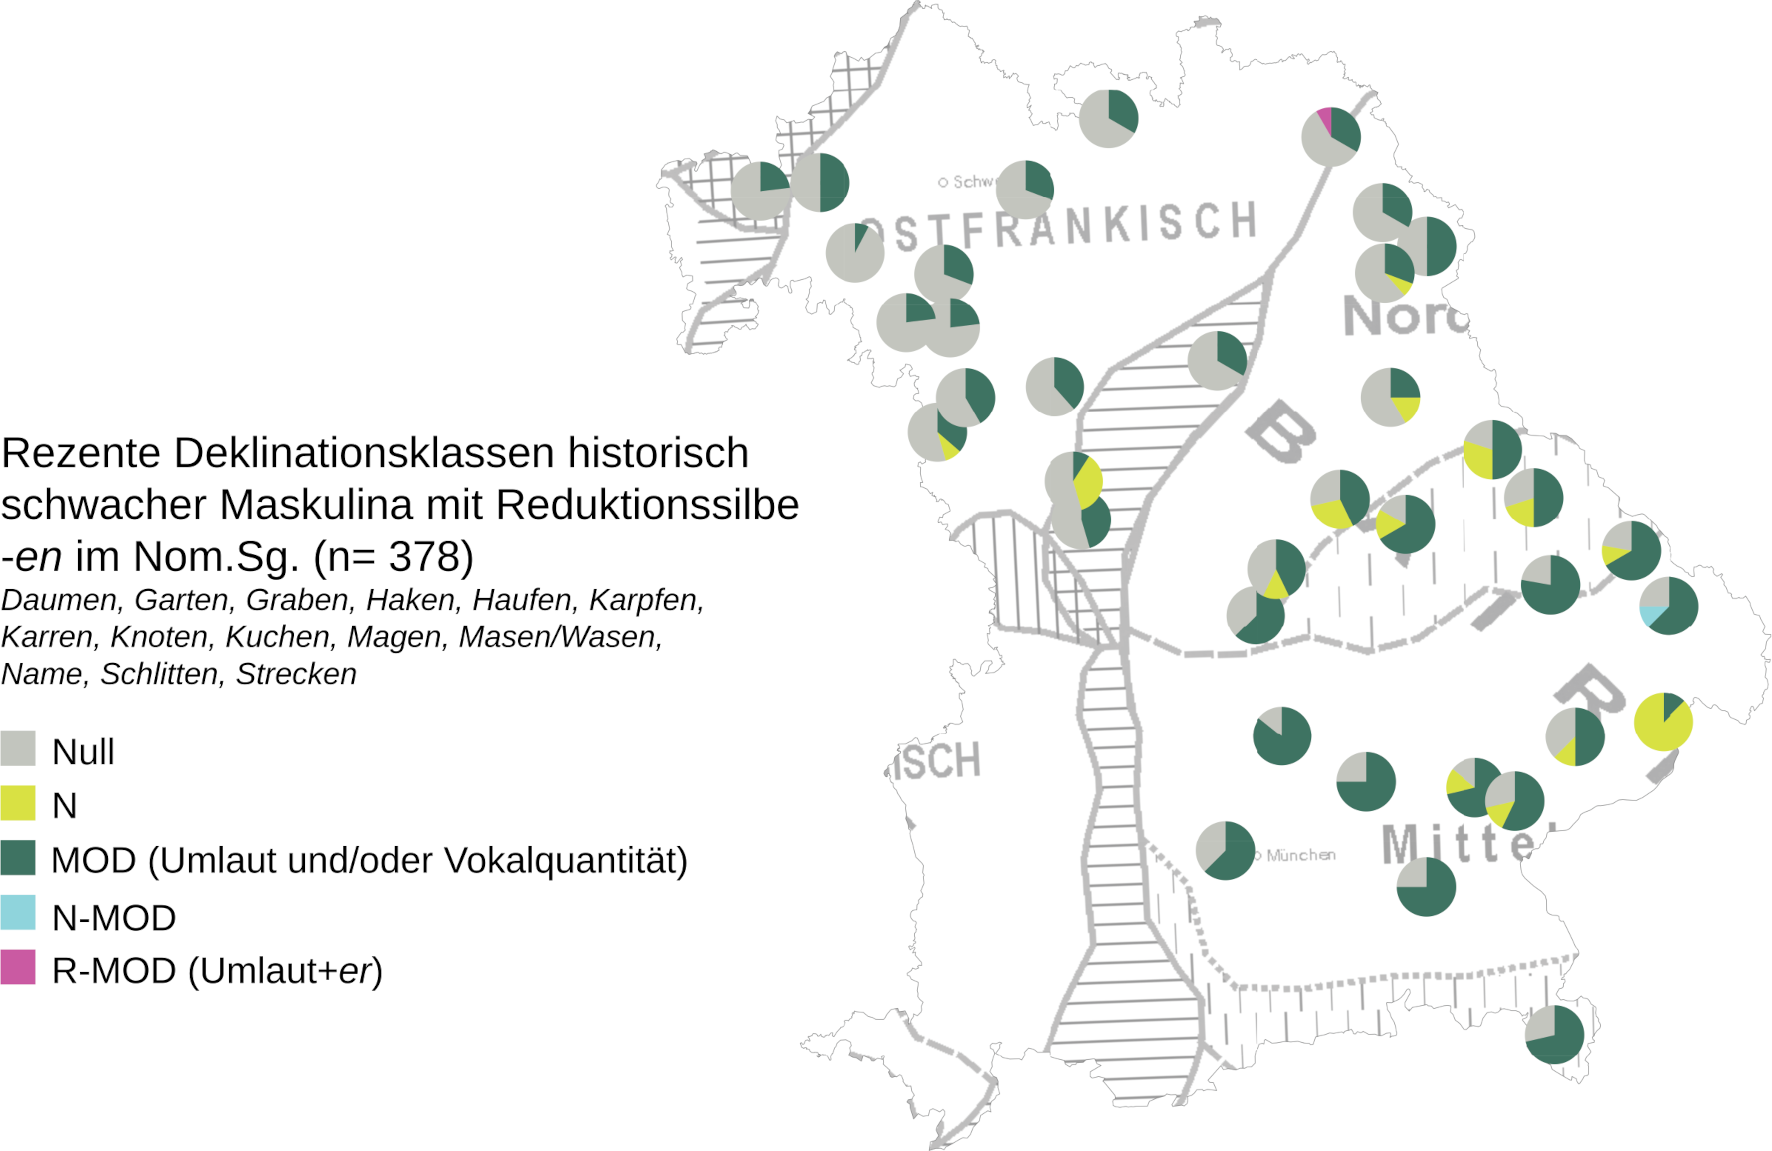
\includegraphics[width=\textwidth]{figures/Karte27.png}
\caption[Rezente Deklinationsklassen historisch schwacher Maskulina, die Reduktionssilbe{}-en im Nom.Sg. aufweisen ]{\label{bkm:Ref53827307}\hypertarget{Toc81223976}{}Rezente Deklinationsklassen historisch schwacher Maskulina, die Reduktionssilbe -\textit{en} im Nom.Sg. aufweisen}
\label{map:27}
\end{map}

\subsection{Neutra}\label{sec:8.2.2}
\begin{sloppypar}
Die Neutra der \textit{a}-Deklination weisen historisch Nullplural auf. Im Mittelhochdeutschen setzt ein Wechsel zur Deklination der historischen \textit{iz/az}{}-Klasse (UL+\textit{er}) oder zum Schwa-Suffix der Maskulina ein, im obd. Sprachraum hindert die Apokope jedoch die analoge Ausbreitung dieses Pluraltyps (vgl. \sectref{sec:3.1.2}). Während einige wenige Neutra (\textit{Fenster}, \textit{Haar}, \textit{Knie}) auch in den rezenten Dialekten im gesamten UG Nullplural aufweisen, sind bei anderen historischen \textit{a}{}-Neutra neben Nullplural auch Deklinationsklassenwechsel in das Pluralverfahren der historischen \textit{iz/az}{}-Klassen belegt (vgl. \citealt[§798]{Schmeller1821}). \textit{Schaf} etwa weist im UG Nullplural auf, nur im nördlichen Nordbair. wird der Plural additiv mit Tiefschwa gebildet (z.\,B. \teuthoo{s\#ôo.<o4v5}{š{\aufstrih}ôͅọv̩} -- \teuthoo{s\#ôo.<o4vA}{š{\aufstrih}ôͅọvα} im nordbair. Groschlattengrün). Im ofr. Erlabrunn (und in einigen weiteren der umgebenden unterofr. Ortsdialekte) findet sich daneben der analoge Umlautplural \teuthoo{s\#o.2Av5}{šōͅαv̩} -- \teuthoo{s\#a9.2v5}{ša\klammeruntenpost{}̄ͅv̩} ‚Schaf‘ (vgl. \citealt[Karte 50]{SBS9.1}). Der his\-to\-ri\-sche \textit{a}{}-Stamm \textit{Bein} ist im Ofr. (Typ \teuthoo{ba2}{bā} -- \teuthoo{di}{di} \teuthoo{ba2}{bā}), vereinzelt auch im Mittelbair. (Typ \teuthoo{boA}{boα} -- \teuthoo{boA}{boα}) mit Nullplural belegt, im Bair. finden sich dagegen Pluralformen mit Tiefschwa (Typ \teuthoo{boA}{boα} -- \teuthoo{boAnA}{boαnα}), im Nordbair. zudem mit dem umlautähnlichen Diphthongwechsel von mhd. \textit{ei} (z.\,B. \teuthoo{bo>+A+}{bỗα̃} -- \teuthoo{bo>+i6nA}{bỗĩnα} im nordbair. Tirschenreuth).\footnote{\citet[131]{Mauser2000} beobachtet in seiner Apparent-time-Studie im Salzburger Lungau Dialektwandel bei den neutralen \textit{a}{}- und \textit{ja}{}-Stämmen: Nullplural entspricht dabei der konservativeren Variante, die von der älteren Generation verwendet wird (z.\,B. \textit{b̥õɐ} -- \textit{b̥õɐ} ‚Bein‘, \textit{ˈhɒˑŋ} -- \textit{ˈhɒˑŋ} ‚Horn‘), während die jüngere Generation die innovativere, numerusdistinkte Varianten realisiere: Pl. \textit{ˈb̥õɐˑnɐ} ‚Beine‘, \textit{ˈhɛˑŋɐ} ‚Hörner‘.} Bei anderen Lexemen (\textit{Fest}, \textit{Seil}, \textit{Sieb}, \textit{Tor}) hat im UG weitgehend ein Wechsel in die Flexion der his\-to\-ri\-schen \textit{iz/az}{}-Klasse stattgefunden, Nullplurale finden sich nur vereinzelt und ohne Raumbildung (vgl. z.\,B. auch \citealt[Karte 14]{SMF7} oder \citealt[Karte 101]{SNiB7}).\footnote{Raumbildung gibt es indes bei der Realisierung des \textit{er}{}-Suffix als konsonantisches \textit{r}{}-Suffix, als Schwa oder Tiefschwa (vgl. \citealt[Karte 52]{SBS9.1}).} Ebenfalls ohne Raumbildung ist die Verteilung der rezenten Deklinationsklassen der historischen \textit{ja}-Stämme \textit{Bett}, \textit{Hemd}, \textit{(Ge-)Leise} und des \textit{a}{}-Stamms \textit{Kummet}, für die jeweils Nullplurale, Entsprechungen des \textit{er}{}-Suffixes und Nasalsuffix belegt sind.\footnote{Bei \textit{Kummet} findet sich einer der wenigen analogen Umlautplurale der Neutra, bezeichnenderweise geht dieser mit Genuswechsel zum Maskulinum einher: \teuthoo{dA}{dα} \teuthoo{k\_a.mAd}{kʰaͅmαd} -- \teuthoo{k\_a.mAd}{kʰaͅmαd} (mit velarisiertem Stammvokal mhd. {\textit{a}} {im Sg. und} hellem \textit{ạ}{}-Laut im Pl.{) im nordbair.-mittelbair. Blaibach.}}
\end{sloppypar}

Insgesamt muss für die Deklinationsklassenwechsel der historischen \textit{a}{}-Neutra diachron Variation und Dynamik angenommen werden, \citet[§798]{Schmeller1821} führt dieses Nebeneinander von Nullpluralen und (neueren) additiven Flexionsformen bei den Neutra auch für die damals rezenten Dialekte Bayerns an. Die diachrone Variation zeigen sowohl die oben aufgezeigten Varianten als auch die morphophonologischen Alternationen, die im UG bewahrt sind. Im Falle des his\-to\-ri\-schen \textit{a}{}-Stammes \textit{Kind} geht \citet[118]{Birkenes2014} davon aus, dass sich die Formen mit analogem \textit{er}{}-Suffix erst im Frühneuhochdeutschen durchgesetzt hat. Formen mit Schwa-Suffix waren \citet[119]{Birkenes2014} zufolge zum Ende des 13. Jahrhunderts im gesamten obd. Raum verbreitet, bedingt durch die einsetzende Apokope verschwinden diese Formen. In den rezenten ofr. und bair. Dialekten finden sich nur noch heteromorphische Varianten des \textit{er}{}-Suffixes. Dass das Schwa-Suffix his\-to\-risch im UG vorhanden war, zeigt synchron die subtraktive Pluralform \teuthoo{khe"+nd}{khẽ̄nd} -- \teuthoo{di}{di} \teuthoo{khen}{khen} im ofr.-hess. Wiesthal (vgl. \citealt[60--61]{Birkenes2014} zur Arealität der verschiedenen Pluralvarianten von \textit{Kind}). Daneben findet sich bei dem \textit{a}{}-Stamm \textit{Bein} neben additiven Formen auch die rein stammaffizierende Form \teuthoo{bo(+>A}{bỗ\klammerobenpost{}α} -- \teuthoo{bo(+>i.}{bỗ\klammerobenpost{}iͅ} im nordbair. Windischeschenbach, deren Diphthongwechsel auf eine historisch zweisilbige Pluralform mit apokopiertem Schwa-Suffix zurückgeht.\largerpage

Die Neutra der historischen \textit{iz/az}-Deklination markieren den Plural mit Umlaut und einer Variante des \textit{er}{}-Suffixes. Teilweise erfolgen daneben Kontraste der Vokalquantität und/oder von Lenis-Fortis-Obstruenten, z.\,B. \teuthoo{do2Av}{dōαv} -- \teuthoo{deEfA}{deəfα} ‚Dorf‘ im nordbair. Tirschenreuth. Innerparadigmatische Alternationen der Vokalqualität, die durch Ein- vs. Zweisilbigkeit der Wortform bedingt waren, führen bei Neutra, die historisch nur \textit{er}{}-Suffix aufwiesen, synchron zu einer Kombination aus \textit{er}{}-Suffix und Alternation der Vokalqualität: Alternationen der Zungenhöhe bei Stammvokal mhd. \textit{e} in Dehnung (z.\,B. \teuthoo{bri9."d}{bri\klammeruntenpost{}̄ͅd} -- \teuthoo{bre4dE}{brẹdə}. ‚Brett‘ im ofr. Burgbernheim) oder umlautähnlicher Diphthongwechsel bei mhd. \textit{ei} (z.\,B. \teuthoo{o\$A}{o̤α} -- \teuthoo{o.iA}{oͅiα} ‚Ei‘ im nordbair.-mittelbair. Bernhardswald).

Anders als im Neuhochdeutschen ist der Umlaut der rezenten Entsprechung der \textit{iz/az}{}-Klasse in den untersuchten Dialekten nicht grundsätzlich konkomitant, d.\,h. Umlaut wird nicht obligatorisch durch das \textit{er}{}-Suffix gefordert bzw. er tritt nicht automatisch ein (vgl. \citealt[82]{Dammel2018}, \citealt[163]{Rowley1997}).\footnote{Anders etwa \citet[§21]{Schübel1955} zum ofr. Dialekt von Stadtsteinach.} So finden sich bei dem his\-to\-ri\-schen \textit{iz/az}{}-Neutrum \textit{Maul} in den bair. Tiefenbohrungspunkten nur Formen ohne Umlaut: \teuthoo{ma24ý}{mạ̄ɫ} -- \teuthoo{ma42l.A}{mạ̄lͅα} (nordbair. Win\-disch\-eschen\-bach) oder -- mit vokalisiertem stammauslautendem /l/ -- \teuthoo{sma.e4}{smaͅẹ} -- \teuthoo{ma4eA}{mạeα} (nordbair.-mittelbair. Blaibach, vgl. \citealt[Karte 32]{SBS9.1}, \citealt[Karten 20, 38]{SMF2.1}). Auch wenn die Diminutivform in beiden Fällen keinen Umlaut aufweist (\teuthoo{ma24l.Adý@}{mạ̄lͅαdɫ̥} in Windischeschenbach, \teuthoo{ma.eAl}{maͅeαl} in Blaibach), so sind der Stammvokal mhd. \textit{û} und der Umlautvokal mhd. \textit{iu} -- anders als etwa die Vokalreihe mhd. \textit{ou}{}-\textit{öu}{}-\textit{ei} (z.\,B. \textit{Baum} -- \textit{Bäume}) -- im bair. Teil des UGs nicht systematisch zusammengefallen. Die Umlautlosigkeit ist im Falle von \textit{Maul} durch den folgenden Konsonanten /l/ bedingt. Vor bestimmten Velar- und Labialkonsonanten, \citet[9b, 49c]{Kranzmayer1956} nennt u.\,a auch /l/, ist der Umlaut bei mhd. \textit{û}, \textit{uo} und \textit{ou} ausgeblieben. Charakteristisch sei bei den umlautenhindernden Konsonanten „die starke Senkung der Hinterzunge“ (\citealt[49e]{Kranzmayer1956}), die die palatale Artikulation der Umlautprodukte behinderte. Der fehlende Umlaut bei \textit{Maul} ist damit schon im Mittelhochdeutschen und durch die phonotaktische Umgebung begründet (ausführlicher hierzu \sectref{sec:8.3.3.2}).\footnote{Der alte \textit{iz/az-}Stamm \textit{Haus} (ebenfalls mhd. \textit{û}) etwa wird in allen Tiefenbohrungspunkte durch UL+\textit{er} markiert (\teuthoo{ha4<o4s}{hậọs} -- \teuthoo{ha4<i.sA}{hậiͅsα} in Windischeschenbach, \teuthoo{A}{α} \teuthoo{ha.2s}{hāͅs} -- \teuthoo{he:2sA}{he{\doubleogonek}̄sα} in Blaibach).} Neben dem historischen \textit{iz/az}{}-Stamm \textit{Maul} finden sich auch bei den alten \textit{a}{}-Neutra \textit{Joch} und \textit{Tor} jeweils Varianten mit und ohne Umlaut, z.\,B. \teuthoo{to.<A}{tôͅα} -- \teuthoo{to.ArA}{toͅαrα} (nordbair.-mittelbair. Grafenkirchen) vs. \teuthoo{s\#do.2dl@do2A}{šdōͅdl̥dōα} -- \teuthoo{de2ArA}{dēαrα} (nordbair. Nabburg), \teuthoo{jo.x}{joͅx} -- \teuthoo{jo.HA}{joͅhͯα} (ofr. Pfofeld) vs. \teuthoo{jo9.x}{jo\klammeruntenpost{}ͅx} -- \teuthoo{jÔe.Xer}{j{\doppelaufstrih}eͅꭗer} (ofr. Gebsattel). Somit hat diachron eine (teilweise phonologisch bedingte) Reorganisation der \textit{iz/az}{}-Klasse stattgefunden, die sowohl die historischen Klassenmitglieder als auch die Klassenwechsler der neutr. \textit{a}{}-Deklination betrifft: in ein Pluralverfahren \textit{er}{}-Suffix, das auch Neutra mit velarem Stammvokal umfasst, und ein Verfahren \textit{er}{}-Suffix mit Alternation der Stammvokalqualität.

Die historisch schwachen Neutra der \textit{n}-Deklination \textit{Auge} und \textit{Ohr} markieren in den rezenten Dialekten den Plural mit Nasalsuffix, im Singularparadigma besteht weitestgehend Kasussynkretismus (vgl. \sectref{sec:7.2.2}, \citealt[88]{Rowley1997}). Deklinationsklassenwechsel in die NULL-Klasse liegt in den bair. Dialekten vor, wo das Nasalsuffix auch in den Nom.Sg. übertragen ist: \teuthoo{sqa2.N}{sʔāͅŋ} -- \teuthoo{a2.N}{āͅŋ} ‚Auge‘ (nordbair.-mittelbair. Blaibach), \teuthoo{s5o.A4n}{s̩oͅα̣n} -- \teuthoo{d5o.<A4n}{d̩oͅα̣n} ‚Ohr‘ (mittelbair. Grafenau, vgl. \citealt[426]{Rowley1990b}). Für eine kleine Gruppe von Neutra liegen Varianten der Pluralmarkierung mit Nasal- und \textit{er}{}-Suffix (ohne Raumbildung) vor: Die historischen \textit{ja}{}-Stämme \textit{Bett}, \textit{Hemd}, \textit{Leise} und der \textit{a}{}-Stamm \textit{Kummet} sind teilweise in die \textit{n}{}-Deklination, das historisch schwache Neutrum \textit{Herz} ist in einem Teil der untersuchten Ortsdialekte zum \textit{er}{}-Plural der historischen \textit{iz/az}{}-Deklination gewechselt.

\subsection{Feminina}\label{sec:8.2.3}
\begin{sloppypar}
Auch bei den starken Feminina der historischen \textit{i}-Deklination schwindet das Schwa-Suffix durch Apokope lautgesetzlich. Feminina dieser Deklination, die den Plural historisch durch UL+\textit{e} markieren, weisen in der Folge in den rezenten Dialekten rein stammaffizierende Pluralformen mit Umlaut auf, z.\,B. \teuthoo{gða.ns}{ɡ̩aͅns} -- \teuthoo{gðens}{ɡ̩ens} ‚Gans‘ (mittelbair. Kirchensur), \teuthoo{va\$osd}{va̤osd} -- \teuthoo{voesd}{voesd} ‚Faust‘ (ofr. Ahorn). Bei historisch kurzem Stammvokal in Dehnung in der einsilbigen Singularform und erhaltener Kürze in der zweisilbigen Pluralform erscheinen Kontraste der Vokalquantität (im Bair. in Kombination mit Lenis-Fortis-Kontrasten). Zum Teil, etwa im Falle von \textit{Faust} (mhd. \textit{û}), erscheinen analogische Quantitätskontraste: \teuthoo{va42o4sd}{vạ̄ọsd} -- \teuthoo{va43i.Sd}{vặiͅʃd} ‚Faust‘ (nordbair. Groschlattengrün), \teuthoo{go2ns}{ɡōns} -- \teuthoo{gðens5}{ɡ̩ens̩} ‚Gans‘ (ofr. Hallerstein). Lautgesetzlich entstanden sind ebenfalls die subtraktiven Pluralformen bei \textit{Hand} im ofr.-hess. Wiesthal und der umlautähnliche Diph\-thong\-wech\-sel von mhd. \textit{ei} bei \textit{Magd} im Nordbair. Im Ofr., wo mhd. \textit{ei} zu \teuthoo{a2}{ạ̄} oder \teuthoo{e2}{ē} monophthongiert ist und infolge der Apokope keine Numerusdistinktion vorliegt, wechselt \textit{Magd} in das Pluralverfahren mit Nasalsuffix (Typ \teuthoo{ma2d}{mād} -- \teuthoo{ma2dn}{mādn}, vgl. \mapref{map:17}). Bei den historischen \textit{i}{}-Stämmen \textit{Bank}, \textit{Hand}, \textit{Wand} ist der Umlaut in die Nominativ-Singular-Form eingedrungen, in der Folge erscheinen Numerussynkretismen (vgl. \sectref{sec:7.1.3.2}). Im bair. Teil des UGs erscheint bei \textit{Bank} und \textit{Wand} sekundäre Numerusdifferenzierung durch Nasalsuffix und damit Deklinationsklassenwechsel, z.\,B. \teuthoo{we+nt}{wẽnt} -- \teuthoo{dswoA}{dswoα} \teuthoo{we+ntn}{wẽntn} ‚Wand‘ im nordbair. Nabburg.
\end{sloppypar}

Ebenfalls in additive Klassen wechseln der historische \textit{i}{}-Stamm \textit{Naht} (Pl. mhd. \textit{næte}) sowie \textit{Nacht}, historisch ein fem. Wurzelstamm, der bereits im Althochdeutschen „spurenweise“ (\citealt[§241]{BrauneHeidermanns2018}) in die \textit{i}{}-Deklination wechselt (ahd. Nom./Akk.Pl. \textit{naht}, mhd. Pl. \textit{naht}, \textit{nehte} neben \textit{nahte}): \textit{Naht} in die N-Klasse (Typ \teuthoo{no2d}{nōd} -- \teuthoo{no2dn}{nōdn}), daneben ist für beide Feminina das kombinierte Verfahren UL+\textit{n} verbreitet, z.\,B. \teuthoo{na:2d5h}{na{\doubleogonek}̄d̩h} -- \teuthoo{ne.2dn}{nēͅdn} ‚Naht‘ im ofr. Wilhermsdorf, \teuthoo{no.xd5\_}{noͅxd̩ʰ} -- \teuthoo{na4X\textsuperscript{«d»}n}{nạꭗ\textsuperscript{d}n} ‚Nacht‘ im mittelbair. Waldhof. Die Pluralform \teuthoo{nôo(+u(+d5}{n{\aufstrih}õ\klammerobenpost{}ũ\klammerobenpost{}d̩} -- \teuthoo{nôo(+u(+nA}{n{\aufstrih}õ\klammerobenpost{}ũ\klammerobenpost{}nα} ‚Naht‘ im nordbair. Oberdolling belegt zudem, dass die spezifisch bair. Outputstruktur auf Nasal+Tiefschwa auch bei Feminina wirksam ist, die historisch (außer im Dat.Pl.) kein Nasalsuffix im Paradigma aufwiesen. Diese Form der Doppelsuffigierung findet sich auch bei dem \textit{i}{}-Stamm \textit{Tür} (\teuthoo{d5e}{d̩e} \teuthoo{d5i“4a}{d̩ị̄a} -- \teuthoo{d5i“4AnA}{d̩ị̄αnα} im mittelbair. Kirchensur), der im gesamten UG in additive Klassen (Nasalsuffix oder eine vokalische Variante) gewechselt ist. Damit erfolgt Deklinationsklassenwechsel in additive Verfahren bei den Feminina der historischen \textit{i}{}-Deklination bei lautgesetzlich oder morphologisch entstandenem Nullplural, aber auch, wie \textit{Nacht} und \textit{Naht} zeigen, bei velarem (d.\,h. umlautfähigem) Stammvokal und altem Umlautplural.

Historisch wiesen die Feminina der {\textit{n}}{{}-} und {\textit{ō}}{{}-Deklination} spezifische Paradigmenkonstellationen auf. Im Laufe des Frühneuhochdeutschen fusionieren beide Klassen zu einer Klasse, der fem. Mischdeklination (siehe 	\tabref{tab:10} und \sectref{sec:3.1.2}). In dieser Phase entsteht im Obd., insbesondere im Bair., ein regional begrenztes Ausgleichsmuster, indem das Nasalsuffix der historisch schwachen Feminina analog in den Nom.Sg. übertragen wird. Bei den fem. \textit{ō}{}-Stämmen, die historisch im Nominativ/Akkusativ Nullplural hatten, wird im Obd. das -\textit{(e)n}{}-Suffix des Gen./Dat.Pl. auf alle Kasus übertragen (vgl. \citealt[83]{KleinEtAl2018}). Diese beiden Paradigmenkonstellationen sind auch in den rezenten Dialekten des UGs zu finden und stellen eine Fortsetzung der historischen Deklinationsklassen dar. Die Singular- und Pluralformen der historischen \textit{ô}{}-Klasse entsprechen dem Typ \teuthoo{bruk}{bruk} -- \teuthoo{brukn}{brukn} ‚Brücke‘ mit apokopiertem Schwa im Singular, die historische \textit{n}{}-Klasse mit dem rezenten Typ \teuthoo{glokN}{ɡlokŋ} -- \teuthoo{glokN}{ɡlokŋ} ‚Glocke‘ weist Numerussynkretismus auf (\sectref{sec:7.1.3.1}, vgl. \citealt[§29.2]{Köhler1934}, \citealt[§35]{Schübel1955}). Eine Reorganisation der beiden Klassen findet dahingehend statt, dass für einzelne Feminina beide Paradigmenkonstellationen belegt sind, wie es exemplarisch das Beispiel \textit{Glocke} in 	\tabref{tab:39} mit den Flexionsmustern (1) und (2) illustriert.\footnote{\citet[§44]{Paul1968} gibt \textit{Glocke} als historisch schwach an, \citet{Lexer1872-1878} dagegen als schwankend.}


\begin{table}
\begin{tabular}{llll@{\,}c@{\,}llll@{\,}c@{\,}l|ll}
\lsptoprule
 & \multicolumn{2}{c}{\textit{n}-Klasse} &  &  & \multicolumn{3}{c}{Dialektale Klassen} &  &  & \multicolumn{2}{c}{\textit{ō}-Klasse} & \\
 \cmidrule(lr){2-3}\cmidrule(lr){6-8}\cmidrule(lr){11-12}
 & {Sg.} & {Pl.} &  & \textbf{${\rightarrow}$} &  & Sg. & Pl.  & \textbf{${\leftarrow}$} &  & \multicolumn{1}{l}{Sg.} & {Pl.} & \\
\midrule
N & \multicolumn{1}{l|}{\textit{zunge}} & \textit{zungen} & N &  & (1) & \teuthoo{glok}{ɡlok} & {\teuthoo{glokN}{ɡlokŋ}} &  & N & {\textit{gebe}} &  & N\\ \cline{2-2}
A &  &  & A &  & (2) & \teuthoo{glokN}{ɡlokŋ} & {\teuthoo{glokN}{ɡlokŋ}} &  & A &  &  & A\\ \cline{12-12}
G &  &  & G &  & \cellcolor{lsLightGray}(3) & \cellcolor{lsLightGray}\teuthoo{glokN}{ɡlokŋ} & \cellcolor{lsLightGray}{\teuthoo{gloknA}{ɡloknα}} &  & G &  & \textit{geben} & G\\
D &  &  & D &  & \cellcolor{lsLightGray}(4) & \cellcolor{lsLightGray}\teuthoo{glokN}{ɡlokŋ} & \cellcolor{lsLightGray}{\teuthoo{glokAn}{ɡlokαn}} &  & D &  &  & D\\
\lspbottomrule
\end{tabular}
\caption{Reorganisation der femininen \textit{n}{}- und \textit{ō}{}-Klasse bei historisch zweisilbiger Singularstammstruktur mit Schwa-Reduktionssilbe in den oobd. Dialekten am exemplarischen Beispiel \textit{Glocke}: Flexionsmuster (1) mit apokopiertem Singularstamm vs. (2) mit \textit{n}{}-erweitertem Singularstamm. Grau schattiert sind sekundäre, additive Pluralformen mit Tiefschwa-Suffix (3) oder Suffixalternation \textit{ŋ} > \textit{αn} (4).}
\label{tab:39}
\end{table}

Bei Feminina, die bereits im Mittelhochdeutschen zwischen \textit{n}{}- und \textit{ô}""-De"-kli"-na"-tion schwanken, stellen variierende Singularstammformen innerhalb eines Ortsdialekts, wie sie beispielsweise \citet[55]{White1966} für das westmittelbair. Eisenhofen angibt, die Fortsetzung der historischen Variation dar: \teuthoo{s\#dro.s}{šdroͅs} neben \teuthoo{s\#dro.sn}{šdroͅsn} -- \teuthoo{s\#dro.sn}{šdroͅsn} ‚Straße‘, \teuthoo{wis}{wis} neben \teuthoo{wisn}{wisn} -- \teuthoo{wisn}{wisn} ‚Wiese‘ (vgl. \citealt[§855]{Schmeller1821}, \citealt[§39a]{Schübel1955}, \citealt[117]{Zehetner1985}).

Daneben erklärt \citet[161]{Rowley1997} die „Konkurrenz“ zwischen Paradigmenkonstellationen (1) und (2) im Raum durch areal variierende Restrukturierungen der fem. Klassen. Demnach bildet das synkretische Paradigma (2) mit \textit{n}{}-erweiterter Singularform in einem nördlichen Streifen des Ofr. eine kleine, geschlossen Deklinationsklasse, während etwa im Bayerischen Wald zwar auch mehr Feminina nach (1) flektieren, das Flexionsmuster (2) aber „keineswegs als geschlossene Flexionsklasse bezeichnet werden kann“ (\citealt[161 und Karte 37]{Rowley1997}).\footnote{Auch nach \citet[15--16]{Mausser1915} sind die apokopierten Formen im Bayerischen Wald und in Teilen Oberbayerns („bis hart an die südbairische Grenze heran“) gebräuchlicher, die \textit{n}{}-erweiterten Formen fänden sich erst im niederbayrischen Flachland. \citet[17]{Mausser1915} führt neben arealer Variation in der Verwendung der beiden Formen auch vertikale Unterschiede an: Die zweisilbigen Formen auf -\textit{a} gälten zumindest in den Dialekten des Bayerischen Waldes als standardnäher, da sie eher der trochäischen Struktur der nhd. Feminina entsprechen.}  Einen weiteren Faktor, der diachron zu einer Reorganisation der Feminina der \textit{n}{}- und \textit{ô}{}-Deklination führt, stellen nach \citet{Rowley1997} semantische Merkmale dar. So flektieren Pflanzenbezeichnungen der historischen \textit{ô}{}-Klasse „weit verbreitet“ \citep[192]{Rowley1997} nach dem Paradigma (2) der schwachen Feminina, während Feminina beider historischer Klassen mit belebtem Denotat im nordbair. Egerland nach dem Muster (1) flektieren, nur Feminina mit dem Merkmal [$-$belebt] weisen im Nom.Sg. Nasalsuffix auf (vgl. \citealt[183]{HarnischRowley1990}). \citet[192]{Rowley1997} zufolge können zumindest die Ausnahmen von den Paradigmen (1) und (2) als direkte Entsprechungen der historischen Zugehörigkeit zur fem. \textit{ô}{}- respektive \textit{n}{}-Klasse durch diese semantischen Bereiche Pflanzen und Lebewesen erklärt werden (siehe auch \citealt[§850]{Schmeller1821}). Als Tendenz ergibt sich dies auch in den untersuchten Dialekten; so werden Baumbezeichnungen beider historischer Klassen weitestgehend mit \textit{n}{}-Erweiterung im Singular realisiert und das historisch schwache Femininum \textit{Katze} in allen Tiefenbohrungspunkten mit apokopiertem Schwa und distinkter Pluralform (Typ \teuthoo{katS}{katʃ} -- \teuthoo{katSn}{katʃn}).\footnote{Zu den Baumbezeichnungen gehören die historisch schwachen Feminina \textit{Birke}, \textit{Buche}, \textit{Erle} und \textit{Lärche} sowie der \textit{ô}{}-Stamm \textit{Eiche} und das im Mittelhochdeutschen schwankende Feminina \textit{Tanne}.}

\begin{sloppypar}
Von dieser Tendenz ausgenommen werden müssen aber einige mittelbair. Ortsdialekte sowie das mittelbair.-südbair. Ramsau, wo Baumbezeichnungen beider historischer Klassen mit apokopiertem Singularstamm realisiert werden (z.\,B. \teuthoo{b5u.Ax}{b̩uͅαx} -- \teuthoo{bu.<AxAn}{bûͅαxαn} ‚Buche‘, \teuthoo{o4a4X!}{ọạꭖ} -- \teuthoo{o4a4X!Y@}{ọạꭖ{\klammerNG}̥} ‚Eiche‘, \teuthoo{d\%a.<n}{d͈âͅn} -- \teuthoo{d\%a.nA}{d͈aͅnα} ‚Tanne‘ in Ramsau). Diese Beobachtung bestätigt sich insgesamt für jene Feminina, die \citet[§44]{Paul1968} oder \citet{Lexer1872-1878} als sicher schwach flektierend ausweisen: Im südlichen Mittelbair. und im mittelbair.-südbair. Übergangsgebiet werden diese mit apokopiertem Schwa und distinkter Pluralform nach dem Paradigma (1) realisiert (\mapref{map:28}). Hier scheint es eine Präferenz für apokopierte Singularstammformen unabhängig von der historischen Klassenzugehörigkeit zur fem. \textit{n}{}- oder \textit{ô}{}-Deklination zu geben, wie auch das Raumbild der \mapref{map:22} zur Singularstammform bei sämtlichen nhd. zweisilbigen Feminina im Korpus bestätigt.
\end{sloppypar}

\begin{map}
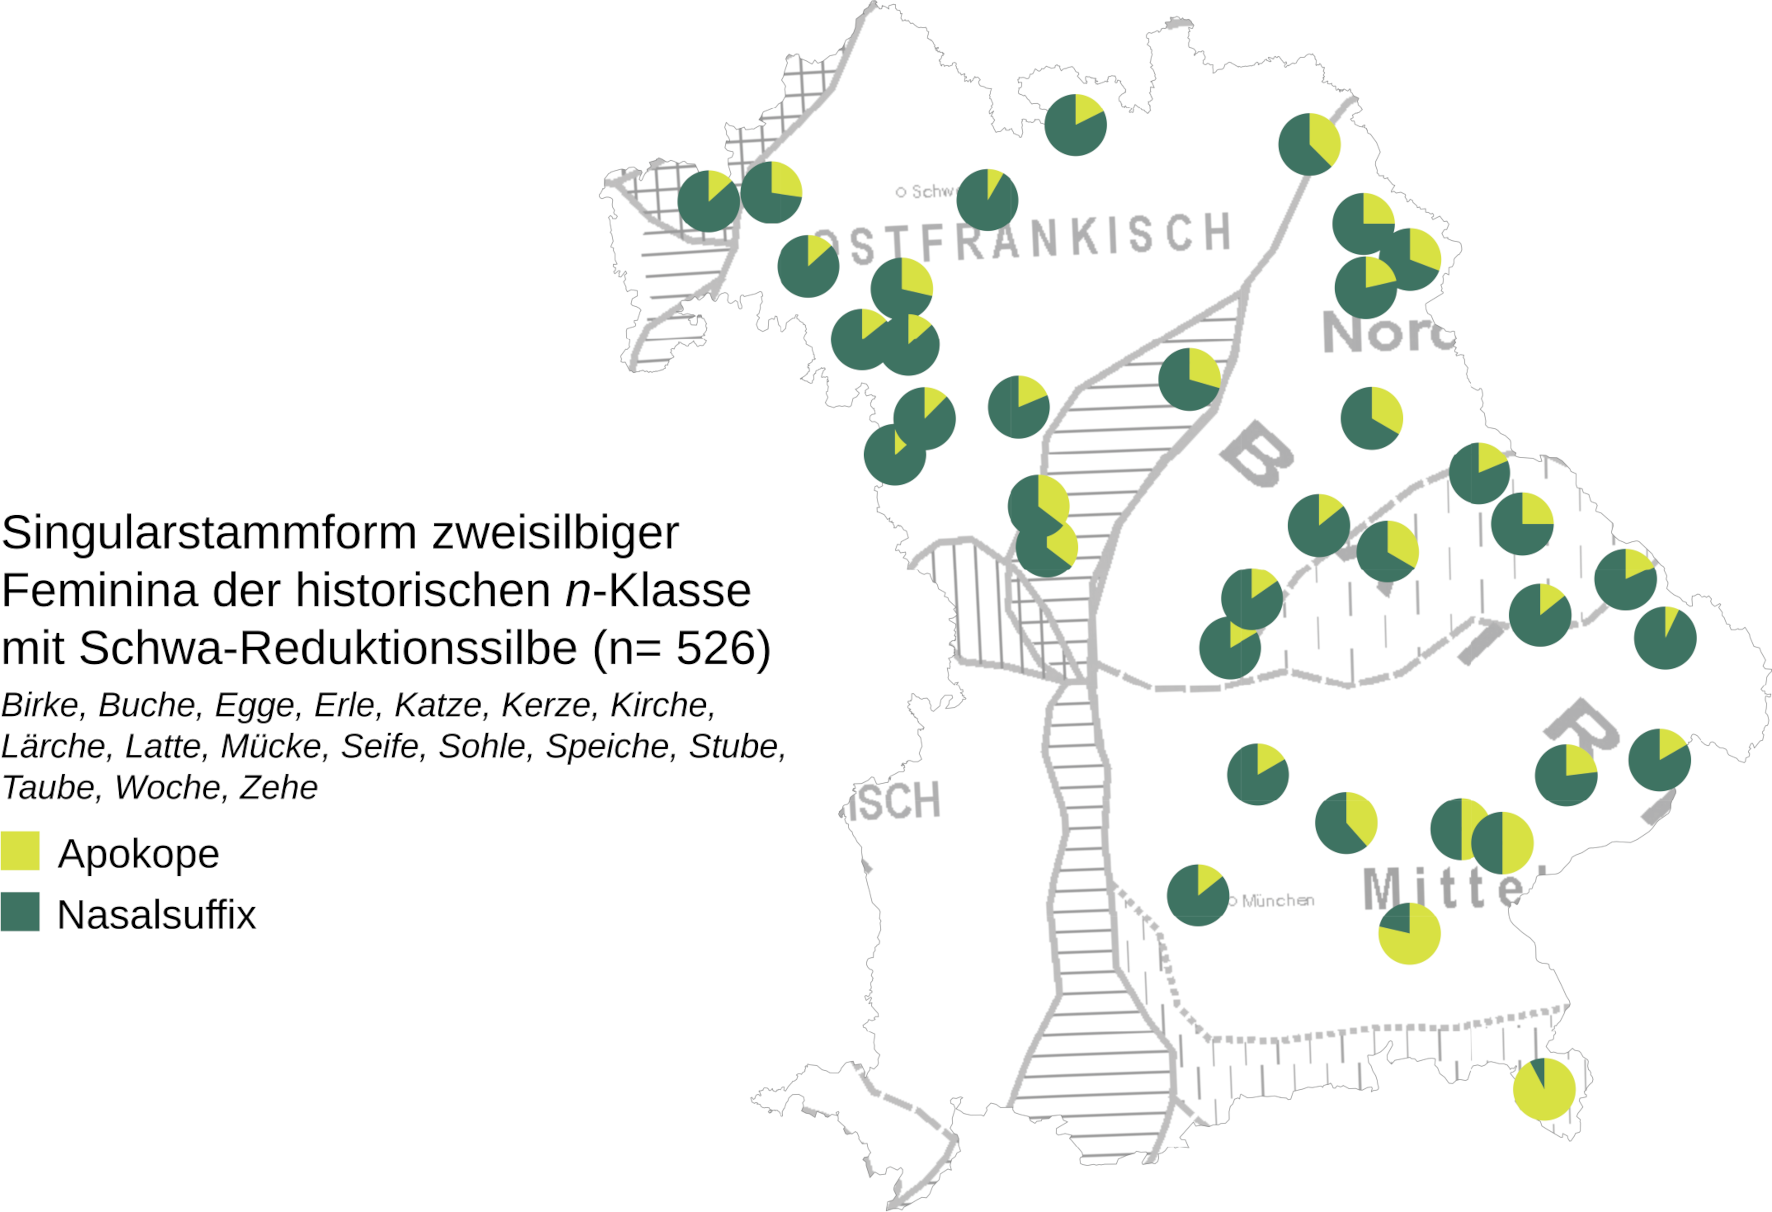
\includegraphics[width=\textwidth]{figures/Karte28.png}
\caption{Singularstammform historisch schwacher Feminina mit Schwa-Reduktionssilbe -- Häufigkeitsverteilung von Apokope vs. \textit{n}{}-Erweiterung im Nom.Sg.}
\label{map:28}
\end{map}

Eine (zumindest in einzelnen Dialekten wirksame) Reorganisation der his"-to"-ri"-schen \textit{n}{}- und \textit{ô}{}-Deklination erfolgt in den untersuchten Dialekten nicht nur im Bereich der Singularstammbildung, sondern auch mit Blick auf die Pluralmarkierung. \tabref{tab:39} weist für das Femininum \textit{Glocke} zwei numerusdistinkte Pluralformen bei \textit{n}{}-erweitertem Singularstamm aus: die additive Markierung mit Tiefschwa-Suffix in Typ (3), die bei vokalisch realisierter \textit{n}{}-Erweiterung als Nasalsuffix realisiert wird (Typ \teuthoo{biEkA}{biəkα} -- \teuthoo{biEkAn}{biəkαn} ‚Birke‘), sowie die Suffixalternation -\textit{n} > -\textit{αn} in Typ (4). Die graue Schattierung markiert, dass beide Verfahren dialektspezifisch für das Bair. sind.

Daneben erfolgt bei einigen Feminina ein Wechsel in die Umlautklasse: im Nordbair., vereinzelt im Ofr. und Mittelbair. \textit{Gabel} (Typ \teuthoo{go2wl}{ɡōwl} -- \teuthoo{ga2wl}{ɡāwl}) und \textit{Wurzel} vereinzelt im Nordbair. (Typ \teuthoo{wuAtS}{wuαtʃ} -- \teuthoo{wiEtS}{wiətʃ} neben \teuthoo{wuAtSl}{wuαtʃl} -- \teuthoo{wiEtSl}{wiətʃl}). Der analoge Umlaut von \textit{Wurzel} wie auch der historisch schwachen Feminina \textit{Mücke} und \textit{Stube}, des \textit{ô}{}-Stamms \textit{Furche} sowie von \textit{Brücke}, im Mittelhochdeutschen zwischen \textit{n}{}- und \textit{ô}{}-Deklination schwankend, ist dabei durch den Stammvokal bedingt. Der Umlaut des Kurzvokals mhd. \textit{u} in geschlossener Silbe ist im Obd. historisch unterblieben oder rückgängig gemacht worden, v.\,a. im nördlichen Oobd. bestand die Tendenz, die Umlautlosigkeit im Singular zu bewahren oder analogisch herzustellen (siehe \sectref{sec:7.1.2.1.1}). Diesen umlautlosen Singularformen stehen Pluralformen mit (analogem oder historischem) Umlaut gegenüber (vgl. 	\tabref{tab:20}). Mit Blick auf die Formenbildung ist interessant, dass reine Umlautplurale bei apokopiertem Singularstamm vor allem im Nordbair. zu finden sind, d.\,h. das Nasalsuffix des Ausgleichsparadigmas der historischen \textit{ô}{}-Deklination erscheint hier nicht: \teuthoo{b,ruk}{b͓ruk} -- \teuthoo{b,rik}{b͓rik} ‚Brücke‘ im nordbair. Nabburg, \teuthoo{vo.rc}{voͅrX} -- \teuthoo{vîirc}{v{\aufstrih}irX} ‚Furche‘ im nordbair.-ofr. Pfofeld, daneben auch analoge Umlautplurale bei \textit{Straße} des Typs \teuthoo{s\#5d5ro.S}{š̩d̩roͅʃ} -- \teuthoo{s\#5d5ra4S}{š̩d̩rạʃ} (mittelbair. Grafenau). Die Kombination aus Umlaut und Nasalsuffix (Typ \teuthoo{go2wl}{ɡōwl} -- \teuthoo{ga2wln}{ɡāwln} oder \teuthoo{s\#droS}{šdroʃ} -- \teuthoo{s\#draSn}{šdraʃn}) und aus Umlaut und Tiefschwa-Suffix (Typ \teuthoo{s\#du.m}{šduͅm} -- \teuthoo{s\#dI2mA}{šdı̄mα}) finden sich (wie auch bei zweisilbigen Maskulina der historischen \textit{i}{}-Deklination, vgl. \sectref{sec:8.2.1}) nur im bair. Teil des UGs (vgl. \citealt[§864]{Schmeller1821}).

Die Feminina der historischen \textit{r}-Klasse, die Verwandtschaftsbezeichnungen \textit{Mutter} und \textit{Tochter}, markieren im Mittelhochdeutschen den Plural mit Umlaut, \textit{Schwester} flektiert nach der fem. Mischdeklination, d.\,h. synkretisches Singularparadigma und Nasalsuffix im Plural (\citealt[§43]{Paul1968}). \textit{Mutter} weist vor allem im Ofr. Umlautplural auf, im bair. Teil des UGs ist der Wechsel in die schwache Flexion mit Nasalsuffix verbreitet (vgl. \citealt[Karte 131]{SNiB7}). Hier müssen zwei unterschiedliche Paradigmenkonstellation unterschieden werden: ein synkretisches Singularparadigma (Typ Sg. \teuthoo{mutA}{mutα} -- Pl. \teuthoo{mutAn}{mutαn}), das v.\,a. im Nordbair. und in Teilen des Ofr. vorkommt, und ein Singularparadigma mit distinkter Dativ-Singular-Form (Typ Nom./Akk.Sg. \teuthoo{mutA}{mutα} -- Dat.Sg. \teuthoo{mutAn}{mutαn} -- Pl. \teuthoo{mutAn}{mutαn}) im südlichen Nordbair. und in Teilen des Mittelbair. (vgl. \mapref{map:25} und \sectref{sec:7.2.2}). In diesem Teil des UGs flektieren \citet[137]{Rowley1997} zufolge auch \textit{Tochter} und \textit{Schwester} schwach (Dat.Sg. \teuthoo{s\#weStan}{šweʃtan}), es handelt sich um den semantisch konditionierten Klassenwechsel in die Deklinationsklasse der Verwandtschaftsbezeichnung, der auch bei den Maskulina stattgefunden hat (vgl. \sectref{sec:8.2.1}).

\textit{Schwester} ist in den BSA-Daten nur in der Nominativ-Singular- und Plural-Form belegt (die Pluralmarkierung erfolgt durch Nasalsuffix), doch zeigen die Wenker-Materialien, dass die schwache Dativ-Singular-Form in diesem Teil des Bair. weit verbreitet und auch in einzelnen Tiefenbohrungspunkte belegt ist, z.\,B. \textit{sag deiner Schwöstern} ‚sag Deiner Schwester‘ im mittelbair. Neukirchen am Inn (vgl. \citealt{WA}-Karte 249 „Schwester“). \textit{Tochter} weist im gesamte UG Umlautplural auf, nur im nordbair. Oberdolling (\teuthoo{do4<xd\%A}{dộxd͈α} -- \teuthoo{de?Xd\%An}{dëꭗd͈αn}) und im mittelbair. Grafenau (\teuthoo{d\%o9.uXtE}{d͈o\klammeruntenpost{}ͅuꭗtə} -- \teuthoo{te.ct;En}{teͅCt͓͓ən}) finden sich die kombinierten Markierungen aus Umlaut und Nasalsuffix, die auch \citet[137]{Rowley1997} für \textit{Tochter} neben \textit{Bruder} anführt; auch hier hat der Wechsel in die schwache Klasse „enge Verwandtschaft“ stattgefunden (vgl. \citealt[Karte 123]{SNiB7}). Die BSA-Daten deuten jedoch daraufhin, dass die schwache Flexion der Verwandtschaftsbezeichnung zum Teil bereits abgebaut ist: Die Gewährsperson im ofr. Hallerstein kennzeichnete die Form \teuthoo{di}{di} \teuthoo{mu.dAn}{muͅdαn} als ‚früher‘ und produzierte selber den Umlautplural \teuthoo{mi.dEr}{miͅdər}.

\section{Konditionierungsprinzipien der dialektalen Deklinationsklassen}\label{sec:8.3}
Die dialektalen Deklinationsklassensysteme werden im Folgenden im Hinblick auf die in \sectref{sec:3.2} eingeführten außerflexivischen Konditionierungsfaktoren analysiert. Ziel ist es zu zeigen, inwiefern Klassenzugehörigkeit und Deklinationsklassenwandel durch diese außerflexivischen Merkmale in den Dialekten konditioniert sind, welche Faktoren überhaupt wirksam sind und ob es dialektspezifische Konditionierungsprinzipien gibt. Da die Untersuchung auf vorhandenen Erhebungsdaten basiert und damit von deren Zusammensetzung abhängig ist, sind Aussagen zu allen bekannten Konditionierungsfaktoren nicht in der Tiefe möglich, wie sie wünschenswert wären (dies betrifft v.\,a. Derivationen und damit morphologische Konditionierung in \sectref{sec:8.3.4}). Gleichzeitig lassen die Daten der BSA-Erhebungen Rückschlüsse auf die Struktur und Zusammensetzung der dialektalen Deklinationsklassen zu. Bedingt durch die unterschiedlichen Forschungsziele der publizierten Sprachatlasbände wurden die Daten nie systematisch dahingehend ausgewertet.

\subsection{Genus}
\label{sec:8.3.1}
Im Standarddeutschen hat sich im Bereich der Pluralallomorphie und genusspezifischer Paradigmenausprägungen eine Schranke zwischen femininen und nicht-femininen Deklinationsklassen herausgebildet (vgl. \sectref{sec:4.1}). Diese Opposition ist das Ergebnis eines Umbaus des Deklinationsklassensystems im Laufe des Frühneuhochdeutschen, der einerseits die Reorganisation der Maskulina und Neutra der historischen \textit{i}{}- und \textit{a}{}-Deklination, anderseits die Herausbildung einer spezifisch fem. Mischdeklination und damit die Ablösung der ahd. Genusschranke zwischen Neutrum und Nicht-Neutrum umfasste (siehe \sectref{sec:3.1.2}). Die in \sectref{sec:8.2} aufgeführten Deklinationsklassenwechsel zeigen, dass sich Genus auch in den untersuchten Dialekten als ein zentraler Steuerungsfaktor der Deklinationsklassenzugehörigkeit erweist. Einzelne Wechselbewegungen und rezente Pluralformen sind allerdings nur in Kombination mit anderen Konditionierungsfaktoren zu erklären.


\begin{figure}
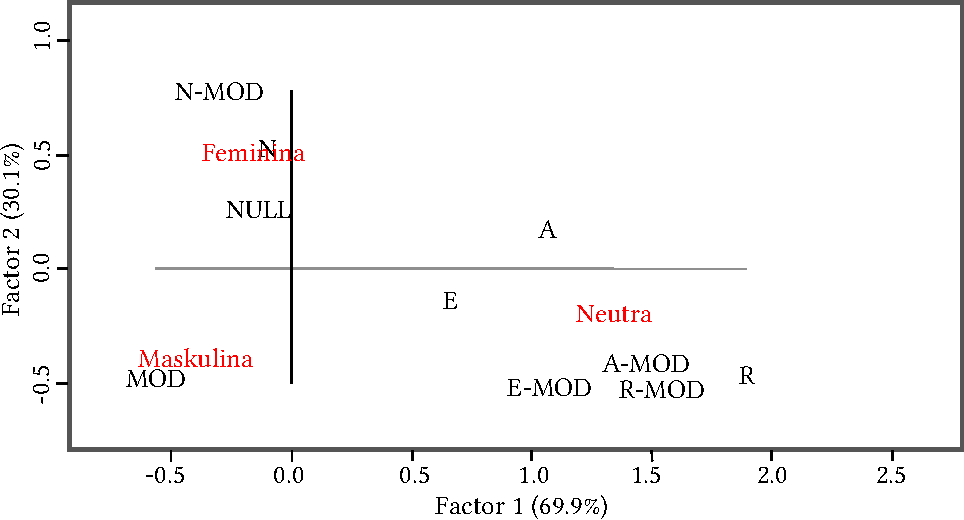
\includegraphics[width=\textwidth]{figures/revisedNickelNominalmorphologie-img044.pdf}
\caption{Korrespondenzanalyse der Variablen Genus und Deklinationsklasse in den untersuchten Dialekten ($n=7943$)}
\label{fig:13}
\end{figure}

\begin{table}
    \begin{tabular}{lrrr}
    \lsptoprule
         &  \multicolumn{3}{c}{Genus}\\
         \cmidrule(lr){2-4}
        DK & Feminina & Maskulina & Neutra\\
        \midrule
        NULL & 1414 & 948 & 316\\
        N & 843 & 312 & 131\\
        A & 159 & 20 & 231\\
        E & 39 & 42 & 63\\
        R & 1 & 4 & 63 \\
        N-MOD & 107 & 27 & 2\\
        A-MOD & 33 & 73 & 348\\
        E-MOD & 9 & 51 & 100\\
        R-MOD & 3 & 33 & 146\\
        MOD & 499 & 1916 & 10\\
        \midrule
        gesamt & 3107 & 3426 & 1410\\
        \lspbottomrule
    \end{tabular}
    \caption{Korrespondenzanalyse der Variablen Genus und Deklinationsklasse in den untersuchten Dialekten ($n=7943$)}
    \label{tabfig:13}
\end{table}

Inwiefern steuert Genus die Pluralallomorphie in den untersuchten Dialekten, inwiefern sind Deklinationsklassen genusspezifisch?  \figref{fig:13} und \tabref{tabfig:13} visualisiert die Häufigkeitsverteilung der Variablen Genus und Deklinationsklasse in Form einer Korrespondenzanalyse mit absoluten Häufigkeiten für das gesamte BSA-Korpus und unter Ausblendung der arealen Dimension.\footnote{Siehe einführend \sectref{sec:7.1.2.3.1} zur Methodik der Korrespondenzanalyse.}  Im relativen Vergleich zeigen die Entfernungen zwischen den einzelnen Variablenausprägungen, dass es Deklinationsklassen gibt, die mit einzelnen Genera korrelieren. Bei Klassen mit additiven Allomorphen ist jeweils die Heteromorph-Ebene beibehalten, d.\,h. Schwa-, Tiefschwa- und \textit{er}{}-Suffix wurden nicht als Heteromorphe des \textit{er}{}-Suffixes, und Schwa-, Tiefschwa- und Nasalsuffix nicht als Heteromorphe des \textit{en}{}-Suffixes abstrahiert. Die relative Entfernung zwischen den einzelnen Variablen auf der rechten Seite der horizontalen Achse weist die R-Klasse und die kombinierten Klassen E-, A- und R-MOD als spezifisch neutrale Klassen aus. Schwa- und Tiefschwa-Suffix (E- und A-Klasse) sind dagegen weniger stark mit den Neutra korreliert, da sie als heteromorphische Varianten des \textit{en}{}- und des \textit{er}{}-Suffixes in den untersuchten Dialekten distribuiert sind, und vokalisch realisierte \textit{en}{}-Plurale auch bei Feminina und Maskulina zu finden sind, etwa bei den \textit{n}{}-erweiterten Feminina (z.\,B. \teuthoo{v5loi).N}{v̩loi\klammeruntenpost{}ͅŋ} -- \teuthoo{vlo<iNA}{vlôiŋα} ‚Fliege‘ im mittelbair. Neukirchen am Inn) oder bei den Maskulina der historisch schwachen Deklination (z.\,B. \teuthoo{ogs5}{oɡs̩} -- \teuthoo{di}{di} \teuthoo{o4gsE}{ọɡsə} ‚Ochse‘ im ofr. Gemünden am Main).

Die linke Seite der horizontalen Achse ist durch Feminina und Maskulina bestimmt, allerdings ist die relative Entfernung beider Genera zueinander weniger groß als zu den Neutra. Auch hier sind einzelne Deklinationsklassen überaus häufig mit den beiden Genera korreliert: die MOD-Klasse mit den Maskulina, N- und NULL-Klasse mit den Feminina. Damit ergibt sich in der Tendenz für das BSA-Korpus insgesamt eine Genusschranke zwischen Neutrum und Nicht-Neutrum. Reduziert man die Datenauswertung von den Heteromorphen, die dialektübergreifend im gesamten UG zu finden sind, auf die Allomorphebene der einzelnen dialektalen Flexionssysteme, so ergeben sich variierende, ortsdialektspezifische Genuskonstellationen zwischen Ofr. und nördlichen Nordbair. einerseits und andererseits den Dialekten des südlichen Nordbair. und Mittelbair. Die Konstellationen, die in  \figref{fig:14a}--\ref{fig:14b} und \tabref{tabfig:14a}--\ref{tabfig:14b} für zwei exemplarische Ortsdialekte gezeigt werden, sind durch einen systematischen Unterschied im Suffixinventar begründet: Werden mhd. -\textit{en} und mhd. -\textit{er} auch im rezenten Flexionssystem unterschieden oder sind mhd. -\textit{en} und mhd. -\textit{er} in Folge der Vokalisierung von mhd. -\textit{en} in bestimmten phonologischen Kontexten zusammengefallen (ausführlicher hierzu \sectref{sec:7.1.1.1})?

Im ofr. Ahorn gibt es zwei additive Allomorphe: Schwa-Suffix als rezente Entsprechung der Reduktionssilbe mhd. -\textit{er} und Nasalsuffix für mhd. -\textit{en}, d.\,h. \textit{er}{}- und \textit{en}{}-Plural werden in diesem Flexionssystem auch synchron unterschieden. Die Streuung der Variablenausprägungen und die relative Entfernung im Plot der Korrespondenzanalyse zeigen wiederum die oben beobachtete Tendenz einer Opposition zwischen Neutrum und Nicht-Neutrum. NULL- und N-Klasse korrelieren überaus häufig mit Feminina, die MOD-Klasse mit den Maskulina und die Klassen E und E-MOD mit den Neutra. Diesen Befund bestätigt auch das Mosaik-Plot, das die Häufigkeitsverteilung der beiden Variablen visualisiert (die Größe der Flächen der Rechtecke ist relativ zur absoluten Häufigkeit zu lesen). N- und NULL-Klasse haben bei den Neutra nur eine periphere Bedeutung, die MOD-Klasse ist nicht vertreten.

In den bair. Dialekten ergibt sich eine andere Distribution von Deklinationsklassen und Genera, da Tiefschwa-Suffix (A-Klasse) als Vokalisierung des \textit{er}{}-Suffixes und als phonotaktisch bedingte vokalische Realisierung von mhd. -\textit{en} „tiefenstrukturell mehrdeutig“ \citep[127]{Rowley1997} ist. Im exemplarisch gewählten Dialekt von Bernhardswald, Übergangsgebiet zwischen südlichem Nordbair. und Mittelbair., weisen die relativen Entfernungen im Korrespondenzanalyse-Plot die
Klassen A-MOD als spezifisch für Neutra und MOD als spezifisch für Maskulina aus. Bemerkenswert ist, dass die Klassen N, NULL und N-MOD zwar stärker mit Femininum korrelieren (und, wie das Mosaik-Plot zeigt, diese in den Klassen auch anteilig am stärksten sind); doch grundsätzlich ist Femininum in allen Deklinationsklassen vertreten.

\begin{figure}
\begin{subfigure}{\textwidth}
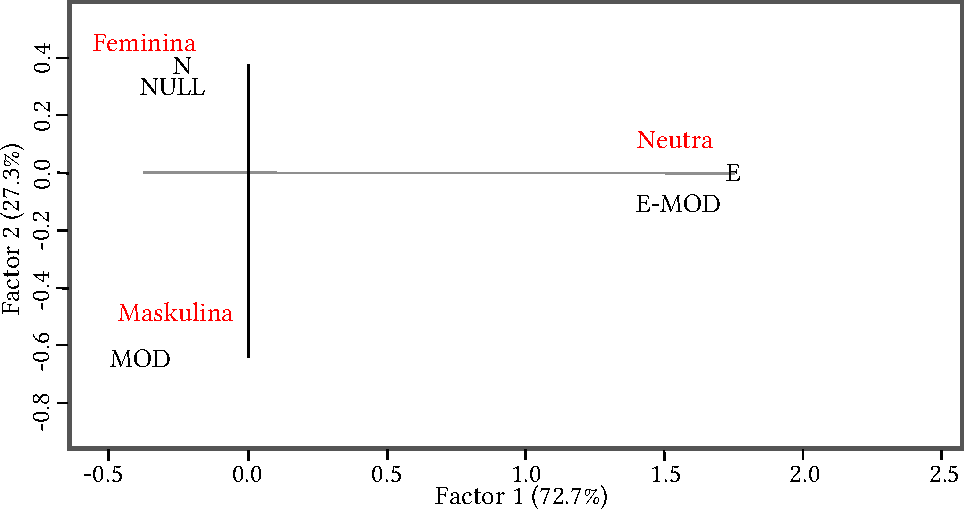
\includegraphics[width=\textwidth]{figures/revisedNickelNominalmorphologie-img045a.pdf}
\caption{}
\label{fig:14a-1}
\end{subfigure}
\begin{subfigure}{\textwidth}
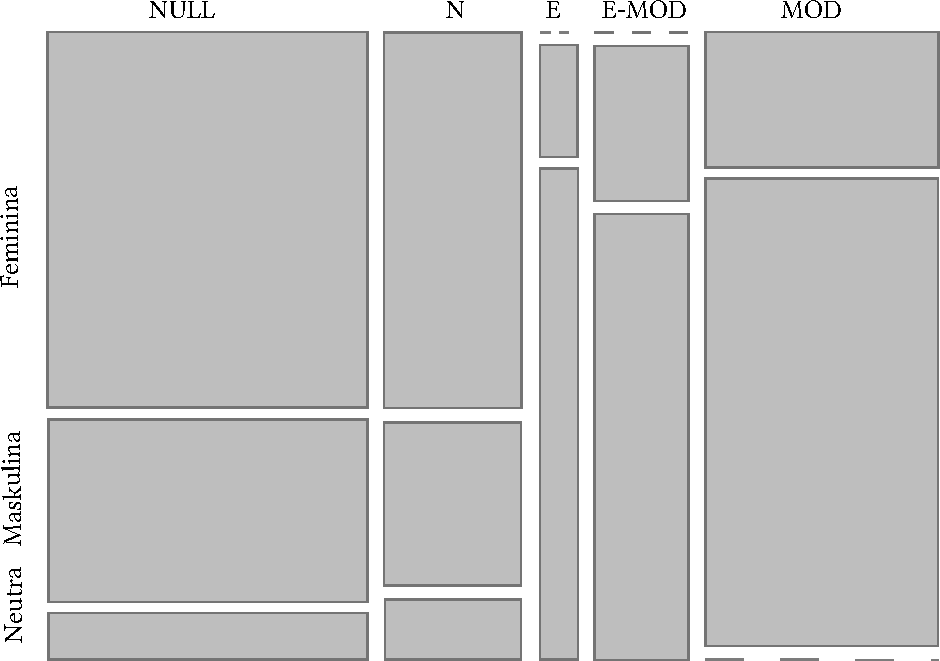
\includegraphics[width=\textwidth]{figures/revisedNickelNominalmorphologie-img045b.pdf}
\caption{}
\label{fig:14a-2}
\end{subfigure}
\caption{Korrespondenzanalyse und Mosaik-Plot der Variablen Genus und Deklinationsklasse in ofr. Ahorn ($n = 239$)}
\label{fig:14a}
\end{figure}

\begin{table}
    \begin{tabular}{lrrr}
    \lsptoprule
         & \multicolumn{3}{c}{Genus} \\
         \cmidrule(lr){2-4}
        DK & Feminina & Maskulina & Neutra\\
        \midrule
        NULL & 58 & 28 & 7\\
        N & 25 & 11 & 4 \\
        E & 0 & 2 & 9 \\
        E-MOD & 0 & 7 & 20\\
        MOD & 15 & 53 & 0\\
        \lspbottomrule
    \end{tabular}
    \caption{Tabelle der Variablen Genus und Deklinationsklasse in ofr. Ahorn ($n = 239$)}
    \label{tabfig:14a}
\end{table}

\begin{figure}
\begin{subfigure}{\textwidth}
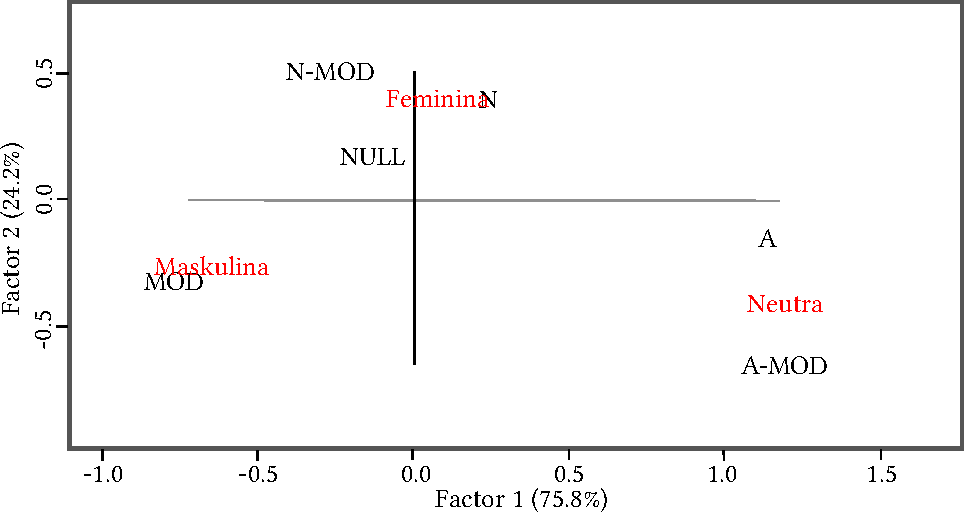
\includegraphics[width=\textwidth]{figures/revisedNickelNominalmorphologie-img045c.pdf}
\caption{}
\label{fig:14b-1}
\end{subfigure}
\begin{subfigure}{\textwidth}
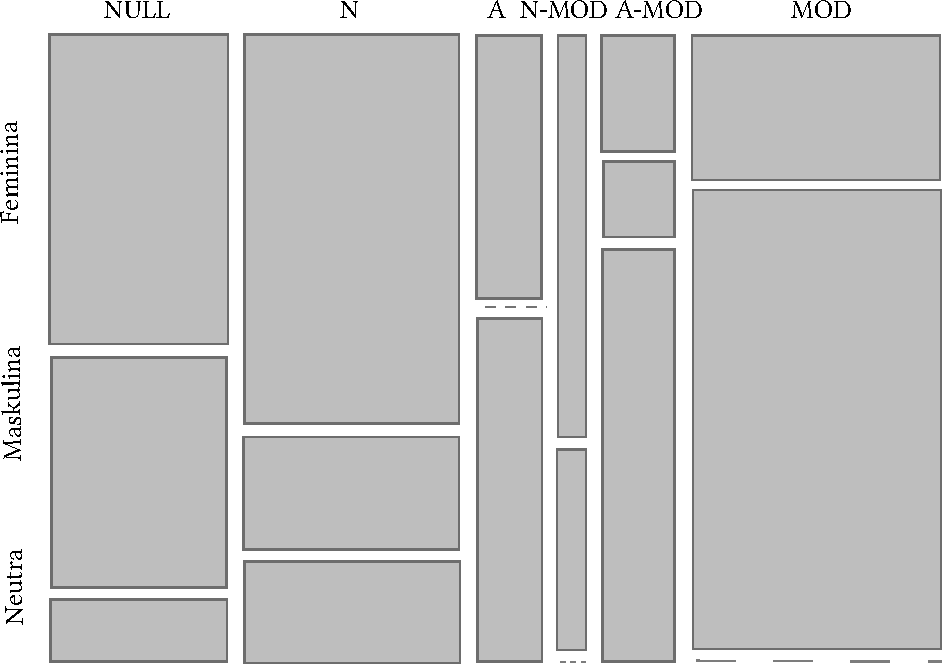
\includegraphics[width=\textwidth]{figures/revisedNickelNominalmorphologie-img045d.pdf}
\caption{}
\label{fig:14b-2}
\end{subfigure}
\caption{Korrespondenzanalyse und Mosaik-Plot der Variablen Genus und Deklinationsklasse in nordbair-mittelbair. Bernhardwald ($n = 178$)}
\label{fig:14b}
\end{figure}

\begin{table}
    \begin{tabular}{lrrr}
    \lsptoprule
         & \multicolumn{3}{c}{Genus} \\
         \cmidrule(lr){2-4}
        DK & Feminina & Maskulina & Neutra\\
        \midrule
        NULL & 20 & 15 & 4\\
        N & 31 & 9 & 8 \\
        A & 6 & 0 & 8 \\
        N-MOD & 4 & 2 & 0\\
        A-MOD & 3 & 2 & 11\\
        MOD & 13 & 42 & 0\\
        \lspbottomrule
    \end{tabular}
    \caption{Tabelle der Variablen Genus und Deklinationsklasse in nordbair-mittelbair. Bernhardwald ($n = 178$)}
    \label{tabfig:14b}
\end{table}

Im Deklinationsklassensystem ergibt sich damit keine eindeutige Opposition zwischen den Genera. Feminina markieren den Plural additiv mit Nasal- und Tiefschwa-Suffix, sodass sie als eine Art Verbindungsglied zwischen dem Nasalsuffix der Maskulina und dem Tiefschwa-Suffix der Neutra stehen. Die Distribution von Nasal- und Tiefschwa-Suffix bei den Feminina und des Nasalsuffixes bei Maskulina und Neutra ist durch dialektspezifische prosodisch-phonotaktische Konditionierungsbedingungen zu erklären (ausführlicher hierzu \sectref{sec:8.3.3}). In diesem bair. Ortsdialekt hat somit eine stärkere Formalisierung der Konditionierung diachron zur Schwächung einer Genusopposition geführt.

Im Folgenden wird die Distribution der Deklinationsklassen für die einzelnen Genera noch einmal zusammengefasst und die dialektspezifische Entwicklung der Feminina als Detailanalyse aufgezeigt.

\subsubsection{Maskulina}
\label{sec:8.3.1.1}
Dialektübergreifend stellen stammaffizierende Verfahren das frequenteste Mittel zur Pluralmarkierung bei den Maskulina dar, die MOD-Klasse ist damit die typenfrequenziell größte Klasse der Maskulina. Stammaffizierende Markierung erscheint als Umlaut bei den Maskulina der historischen \textit{i}{}-Deklination, als analoger Umlaut bei Klassenwechslern (etwa aus der historischen \textit{a}{}-Klasse) und in Form von lautgesetzlich entstanden Kontrasten der Vokalquantität und -qualität und des Konsonantismus oder als Kombination dieser Verfahren (vgl. \sectref{sec:8.2.1}). Infolge der Öffnung des UL+\textit{er}{}-Verfahrens der neutralen \textit{iz/az}{}-Klasse für Maskulina erscheint Umlaut bei einzelnen Lexemen in Kombination mit einer heteromorphischen Variante des \textit{er}{}-Suffixes (z.\,B. bei \textit{Dorn}, \textit{Halm}, \textit{Wurm}).

Nullplural findet sich bei einsilbigen, vor allem aber bei zweisilbigen Stämmen auf -\textit{en}, -\textit{el}, -\textit{er}. Hier sind jene Dialekte des südlichen Nordbair. und Mittelbair. ausgenommen, in denen eine prosodisch-phonotaktische Inputkonditionierung die additive Pluralmarkierung durch Nasalsuffix bedingt: ofr. \teuthoo{s\#liSl@}{šliʃl̥} -- \teuthoo{s\#liSl@}{šliʃl̥} vs. bair. \teuthoo{s\#liSl@}{šliʃl̥} -- \teuthoo{s\#liSl@n}{šliʃl̥n} ‚Schlüssel‘ (ausführlicher hierzu \sectref{sec:8.3.3.1}). Während die Nasalsuffigierung in diesen Fällen durch formale Konditionierung gesteuert ist, sind die übrigen Mitglieder der N-Klasse historisch schwache Maskulina (darunter \textit{Bauer}, \textit{Hase}, \textit{Ochse}). Teilweise, vor allem in den nordbair. Dialekten, finden sich zudem Klassenwechsler mit dem semantischen Merkmal [+belebt] (siehe \sectref{sec:8.3.2.2}). Wiederum im bair. Teil des UGs sind vereinzelt auch Maskulina in der A-Klasse vertreten, etwa \teuthoo{s\#doA}{šdoα} -- \teuthoo{s\#doAnA}{šdoαnα} ‚Stein‘ oder \teuthoo{bou}{bou} -- \teuthoo{boumA}{boumα} ‚Bube‘; die Suffigierung mit Tiefschwa in der Abfolge Nasal+α entspricht hier einer präferierten, dialektspezifischen prosodischen Outputstruktur des Bair.

\subsubsection{Neutra}
\label{sec:8.3.1.2}
Als spezifische Klassen der Neutra erweisen sich dialektübergreifend die rezenten Entsprechungen der historischen \textit{iz/az-}Deklination, R und R-MOD (bzw. deren heteromorphische Varianten), sie stellen die typenfrequentesten Klassen der Neutra dar. Diachron hat eine (zum Teil phonologisch bedingte) Reorganisation der \textit{iz/az}{}-Klasse stattgefunden, in der Folge ist der Umlaut bei \textit{er}{}-Suffigierung bei historischen \textit{iz/az}{}-Neutra und Klassenwechslern nicht grundsätzlich konkomitant (vgl. \sectref{sec:8.2.2}). Auch \citet[163]{Rowley1997} beobachtet „den Ansatz einer Verselbständigung“ des \textit{er}{}-Plurals ohne Umlaut in seinem nordostbayerischen UG. Als weitere additive Klasse ist die N-Klasse bei den wenigen historisch schwachen Neutra (\textit{Auge}, \textit{Ohr}, \textit{Herz}) sowie teilweise bei den alten \textit{a}{}- und \textit{ja}{}-Stämmen \textit{Bett}, \textit{Hemd}, \textit{Leise}, \textit{Kummet} belegt. Daneben weisen die zweisilbigen Diminutiva auf \textit{el}{}-Reduktionssilbe der prosodisch-phonotaktischen Inputkonditionierung entsprechend im südlichen Nordbair. und vereinzelt im Mittelbair. Nasalsuffix auf, daneben auch die Diminutiva mit Derivationssuffix -\teuthoo{XE}{ꭗə} im ofr.-hess. Wiesthal (siehe \sectref{sec:8.3.3.1} sowie \sectref{sec:8.3.4} zur morphologischen Konditionierung). Nullplural weisen hingegen nur einige historische \textit{a}{}-Stämme auf (\textit{Fenster}, \textit{Haar}, \textit{Knie}, teilweise \textit{Schaf}) sowie die historischen \textit{n}{}-Stämme \textit{Auge} und \textit{Ohr} mit Nasalsuffix im Nom.Sg. im Bair. (vgl. \sectref{sec:8.3.2.1}).

\subsubsection{Feminina}
\label{sec:8.3.1.3}
Im gesamten UG weisen die historischen \textit{i}{}-Stämme auch in den rezenten Dialekten stammaffizierende Markierung auf, zudem sind einige analoge Umlautplurale in der MOD-Klasse zu finden, etwa bei \textit{Gabel}, \textit{Mücke} oder \textit{Straße} (siehe \sectref{sec:8.2.3}). Im bair. Teil des UGs erscheinen alte und analoge Umlautplurale in Kombination mit Nasalsuffix (Klasse N-MOD), und zwar sowohl bei einsilbigem (häufig apokopiertem) Singularstamm oder bei zweisilbigen Stämmen.

Eine Zweiteilung des UGs ergibt sich bei der typenfrequenten Klasse der his\-to\-ri\-schen \textit{n}{}- und \textit{ô}{}-Stämme, die in den rezenten Dialekten mit apokopierter Singularform oder mit Nasalsuffix im Nom.Sg. realisiert werden. Im gesamten UG markieren apokopierte Stämme den Plural regelmäßig mit Nasalsuffix (d.\,h. N-Klasse); ausgenommen werden müssen hier apokopierte Feminina mit kollektiver Semantik (etwa \textit{Bremse}, \textit{Birne}, \textit{Kirsche}, \textit{Klaue}), die dialektübergreifend, vor allem aber im südlichen Nordbair., häufig Nullplural aufweisen (Typ \teuthoo{erwEs}{erwəs}-- \teuthoo{erwEs}{erwəs} ‚Erbse‘, ausführlicher hierzu \sectref{sec:8.3.2.1}). Eine dialektraumspezifische Form der Pluralmarkierung findet sich indes bei den Feminina mit \textit{n}{}-Erweiterung. Hier liegt auch die Lösung begründet für die eingangs beobachtete variierende Genuskonstellation zwischen den Dialekten des südlichen Nordbair. und des Mittelbair. sowie dem Ofr. und nördlichen Nordbair.

In \mapref{map:29} ist die absolute Häufigkeit der numerussynkretischen NULL-Klas\-se (links) und der numerusdistinkten Klassen N und A (rechts) bei \textit{n}{}-erweiterten Feminina gegenübergestellt. Differenziert wurde zudem die Form der Reduktionssilbe (Nasal vs. vokalische Realisierung des Nasalsuffixes). Die Raumbildung zeigt, dass die additive Markierung der \textit{n}{}-erweiterten Feminina sowohl nach Nasal- als auch nach Tiefschwa-Suffix ein Spezifikum des südlichen Nordbair. und des Mittelbair. ist.\footnote{Vgl. hierzu auch die Raumbildung von \citealt{WA}-Karte 72 „Wochen“. Bemerkenswert ist hier, dass die distinkte Pluralform im Abfragekontext des Wenker-Satzes nach einer Zahlenangabe erfolgt, wo sie in den untersuchten Dialekten regelmäßig unterbleibt, beispielsweise im nordbair.-mittelbair. Zwiesel: \textit{Er is vor vie oder fünf Wochan gstoam} ‚Er ist vor vier oder fünf Wochen gestorben‘ (vgl. \sectref{sec:8.3.2}).} Zwar weisen auch die Dialekte des westlichen Ofr. vokalisierte Reduktionssilben auf, doch erscheint hier eine additive Markierung nicht systematisch.

\begin{map}
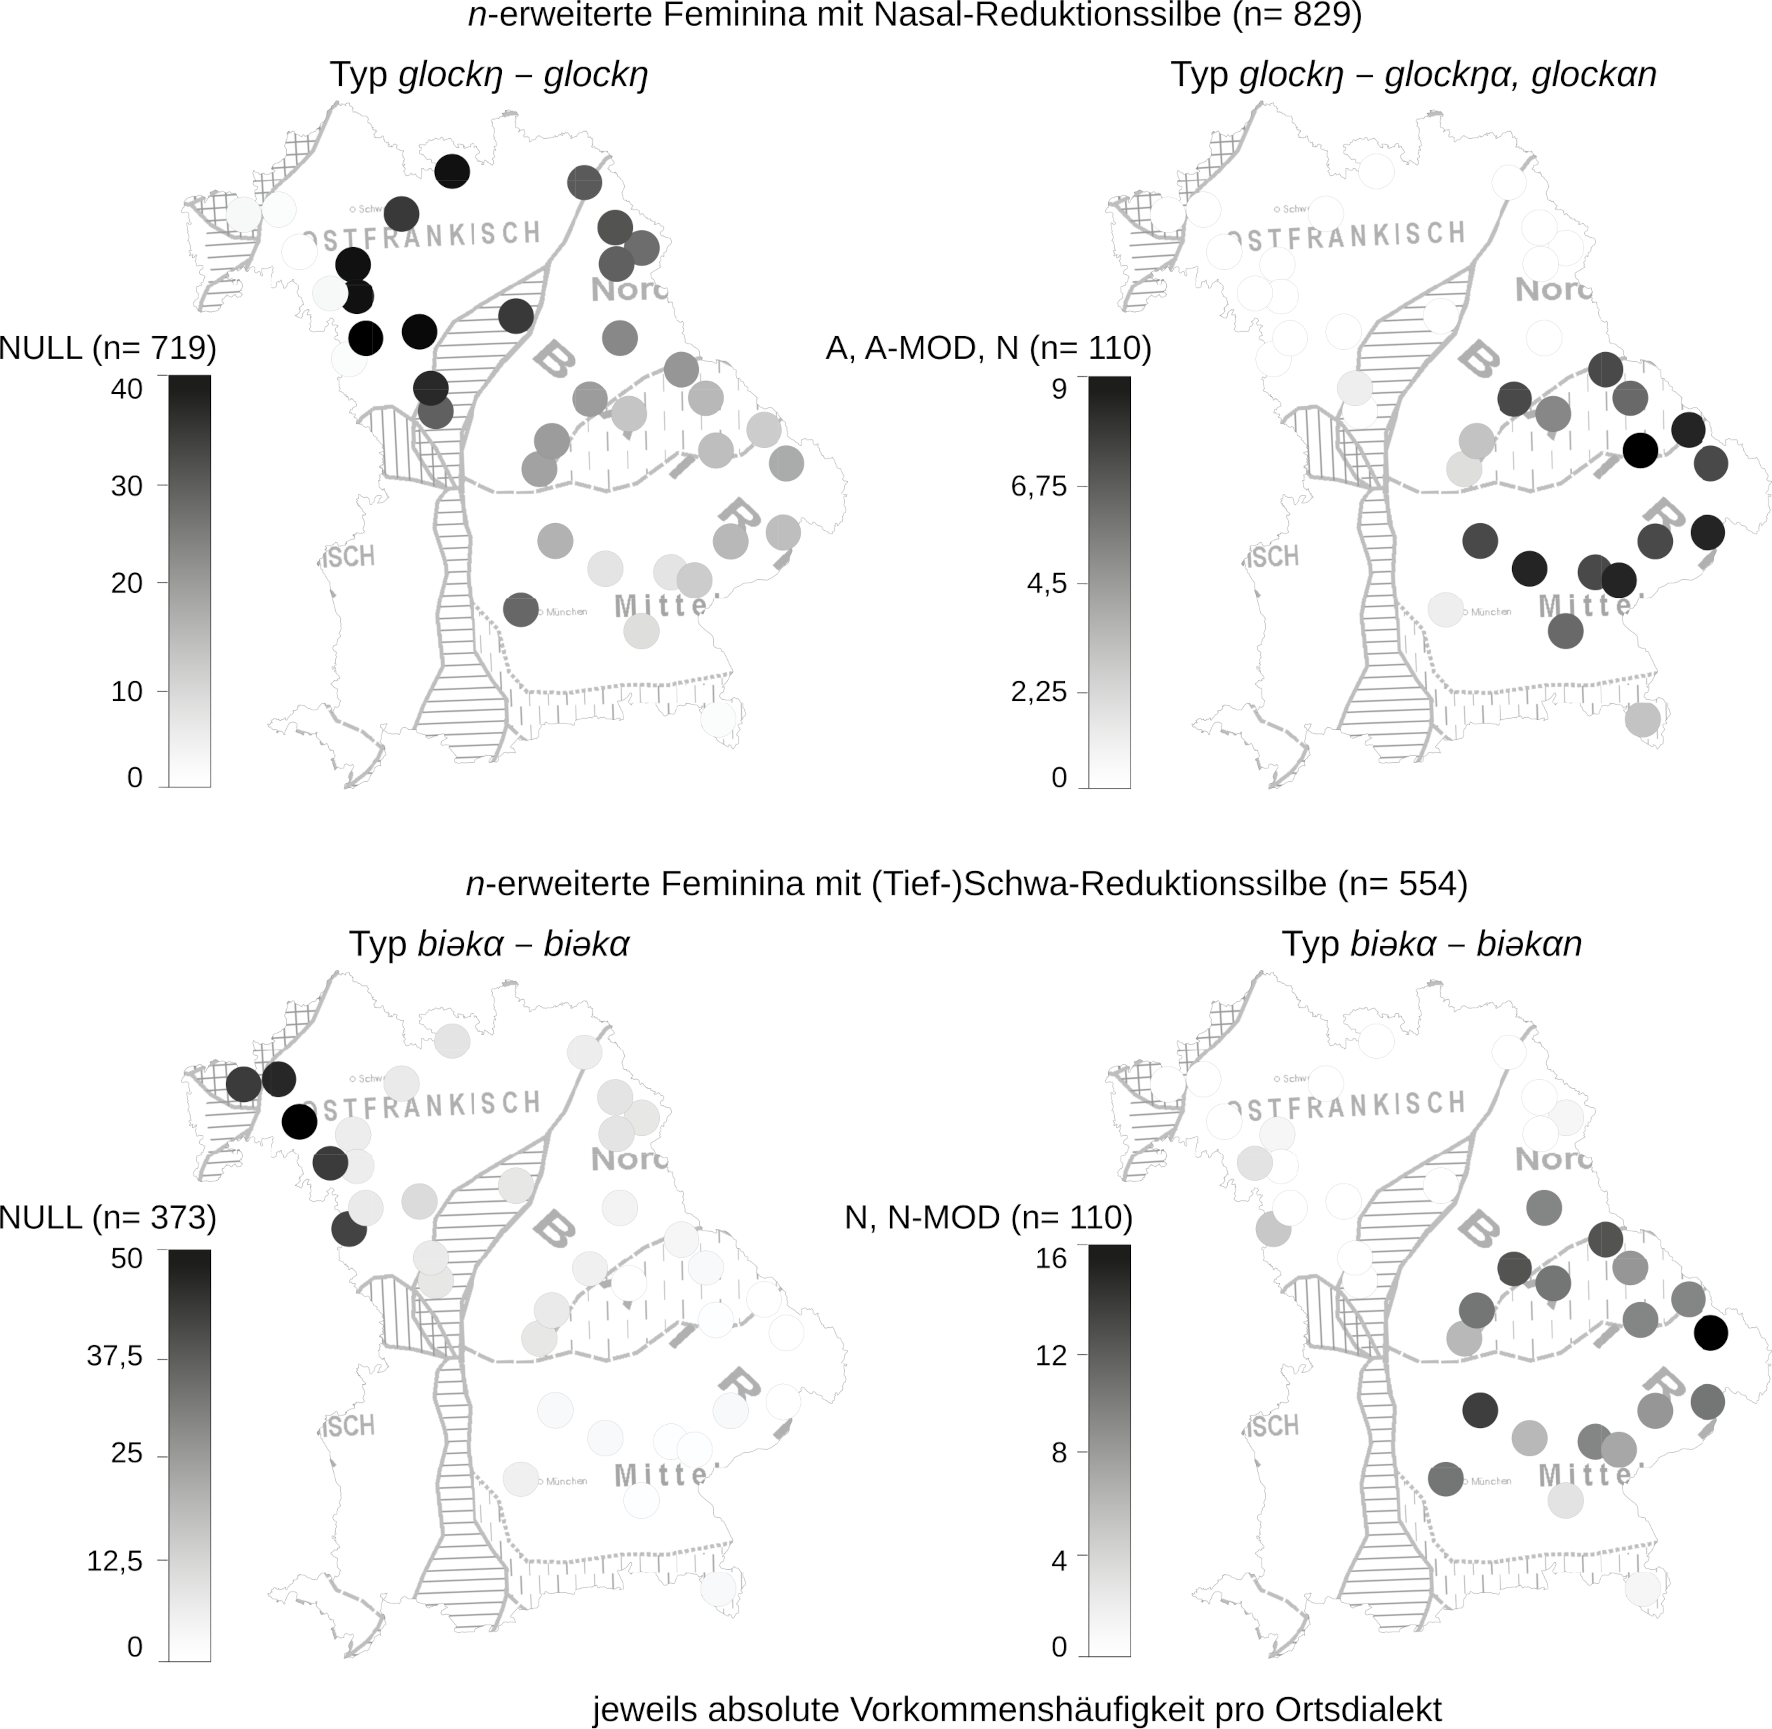
\includegraphics[width=\textwidth]{figures/Karte29.png}
\caption{Areale Häufigkeitsverteilung der Deklinationsklassen NULL, A, N bei \textit{n}{}-erweiterten Feminina ($n=1.383$)}
\label{map:29}
\end{map}


Die Distribution von Tiefschwa- und Nasalsuffix ist im Bair. phonotaktisch durch die Form des Nasalsuffixes im Nom.Sg. konditioniert. Daneben bildet Tief\-schwa-""Re\-duk\-tions\-sil\-be eine produktive Inputbedingung für Nasalsuffigierung und die Abfolge aus Nasal+Tiefschwa-Suffix eine produktive Outputstruktur in diesem Dialektraum (siehe \sectref{sec:8.3.3}). In den Flexionssystemen, in denen Tiefschwa-Suffix ein produktiver Pluralmarker der Feminina (neben den Neutra) ist und zumindest teilweise eine Formalisierung der Konditionierungsprinzipien der Pluralallomorphie erfolgte, ist die Genusopposition zwischen Neutrum und Nicht-Neutrum in der Folge geschwächt.

\subsection{Semantik}\label{sec:8.3.2}
\begin{sloppypar}
Semantische Konditionierung ist von der in \sectref{sec:8.3.3} behandelten formalen Konditionierung zu unterscheiden, da sich semantische Konditionierungsprinzipien auf Merkmale der Inhaltsseite des sprachlichen Zeichens beziehen, während formale Konditionierung die Ähnlichkeit von Merkmalen der Ausdrucksseite betrifft. Eine semantische Steuerung von Deklinationsklassen ist da zu beobachten, wo sich Substantive mit gleichen semantischen Merkmalen auch in der Flexion gleich verhalten. Semantische Distinktionen, die bereits das Deklinationsklassensystem der historischen Vorstufen des Deutschen konditionierten (etwa das besondere flexivische Verhalten von Verwandtschaftsbezeichnungen der historischen \textit{r}{}-Klasse), sind auch in den rezenten Dialekten zu finden. Daneben stellen semantische Distinktionen auch diachron einen Konditionierungsfaktor dar, der einerseits die Reorganisation einzelner Deklinationsklassen und anderseits die Distribution von Allomorphen steuert (vgl. \sectref{sec:3.1.2} sowie den Überblick in \citealt[100--104 und 116--122]{Kürschner2008a}).
\end{sloppypar}

Dass die Abgrenzung genuin semantischer Konditionierung methodisch nicht unproblematisch ist, zeigen \citet{VerslootAdamczyk2018} in ihrer Studie zur irregulären Flexion in den nordseegermanischen Varietäten, indem sie die Brücke zwischen semantischer Steuerung, Analogiebildungen und Kognition schlagen. Die Assoziation von ähnlichen semantischen Merkmalen führt zu Deklinationsklassenwechseln, wenn etwa der historische \textit{i}{}-Stamm \textit{Fisch} (engl. \textit{fish} -- \textit{fish}) analogisch den Nullplural des historischen \textit{a}{}-Neutrums \textit{Schaf} (engl. \textit{sheep} -- \textit{sheep}) annimmt (vgl. \citealt[49--50]{VerslootAdamczyk2018}). Beide Lexeme gehören zu einer semantischen Klasse von Substantiven, die Tiere denotieren und (neben Personen- und Körperteilbezeichnungen) eine hohe absolute und relative Häufigkeit irregulärer Pluralformen aufweisen. Infolge der Korrelation spezifischer semantischer Merkmale und irregulärer Pluralmuster entsteht kognitiv eine „activation relation“ (\citealt[50]{VerslootAdamczyk2018}) zwischen semantischer Kategorie und Pluraltyp: Immer dann, wenn eine spezifische irreguläre Pluralform produziert wird, wird die semantische Kategorie im Gehirn koaktiviert. Bemerkenswert ist hier, dass die Assoziation ähnlicher semantischer Merkmale die eigentlich durch die Vorkommenshäufigkeit bedingte Überrepräsentation irregulärer Pluralformen überdeckt: „For the synchronic (statistical) language learner, the diachronic causal relations are irrelevant; it is rather the model [Regressionsmodell, GN] which includes semantics as an independent variable that represents the learner’s reality“ (\citealt[50]{VerslootAdamczyk2018}). Methodisch besteht daher eine Schwierigkeit darin, die steuernde Wirkung von semantischen Distinktionen von Frequenzeffekten abzugrenzen, da Semantik und hohe Frequenz einander bedingen können (\citealt[26]{VerslootAdamczyk2018}).

Als steuernde Faktoren wurden in dialektologisch-grammatischen Darstellungen die folgenden semantischen Distinktionen identifiziert:

\begin{itemize}\sloppy
\item Nach einem Zahlwort weisen vor allem \textit{Maß-} \textit{und} \textit{Mengenangaben} keine Pluralmarkierung auf, z.\,B. ofr. \teuthoo{drai}{drai} \teuthoo{maus}{maus} \teuthoo{bøiEr}{bøiər} ‚drei Maß Bier‘ oder \teuthoo{tse2.a.}{tsēͅaͅ} \teuthoo{fas}{fas} \teuthoo{wa.i.}{waͅiͅ} ‚zehn Fass Wein‘ (\citealt[§279]{Gebhardt1907}). Nach \citet[105]{Rowley1997} erscheint die unflektierte Singularform nach Zahlwörtern auch bei jenen Substantiven, die in anderen morphosyntaktischen Kontexten eine „besondere Pluralbildung“ haben: ofr. \teuthoo{o.n}{oͅn} \teuthoo{di}{di} \teuthoo{viEdsic}{viədsiX} \teuthoo{haus}{haus} ‚an die vierzig Haus‘.\footnote{Hierzu zählen u.\,a. die Zeiteinheiten \textit{Jahr} und \textit{Tag}, „mancherorts“ \citep[188]{Rowley1997} auch \textit{Woche} (für eine exhaustive Liste siehe \citealt[188]{Rowley1997}). \citet[78]{Wittmann1943} und \citet[318]{Schiepek1908} führen daneben \textit{Nacht} als Zeiteinheit ohne Pluralmarkierung an (gegenüber dem regulären Umlautplural), z~B. \textit{ál Tōch} ‚alle Tage‘, \textit{ál Nācht} ‚alle Nächte‘ (vs. Pl. \textit{Tāch}/\textit{Tēch} bzw. \textit{Nácht}, \citealt[318]{Schiepek1908}).} \citet[§279]{Gebhardt1907} bietet einen Beleg für diese Form morphosyntaktisch bedingter Varianz aus dem Nürnberger Dialekt: ofr. \teuthoo{nau}{nau} \teuthoo{warn}{warn} \teuthoo{di}{di} \teuthoo{leXEr}{leꭗər} \teuthoo{na4igmåxt}{nạiɡm{\burgeroalpha}xt}: \teuthoo{a.2}{āͅ} \teuthoo{lu2x}{lūx}, \teuthoo{tswa2}{tswā} \teuthoo{lu2x}{lūx}, \teuthoo{drai}{drai} \teuthoo{lu2x}{lūx}, \teuthoo{føiEr}{føiər} \teuthoo{lu2x}{lūx} ‚Jetzt werden die Löcher hineingemacht: ein Loch, zwei Loch, drei Loch, vier Loch‘.
\item Das semantische Merkmal \textit{Vorkommen} \textit{in} \textit{Menge} oder \textit{in} \textit{Scharen} und auch das Vorkommen als \textit{Paar} konditioniert im südlichen Nordbair. Nullplural (\citealt[102]{Denz1977}, \citealt[§140.6]{Kollmer1987}, \citealt[148, 159]{Rowley1997}).
\item Im nördlichen Randstreifen des Ofr. sind verschiedene Ausprägungen einer Konditionierung der Deklinationsklasse durch die Distinktionen [${\pm}$\textit{be\-lebt}] und [${\pm}$\textit{menschlich}] belegt (\citealt{HarnischRowley1990}, \citealt[191]{Rowley1997}). Daneben steuert das Belebtheitsmerkmal Klassenwechsel in die schwache Deklination (vgl. \citealt[§20--21]{Micko-Repp1933}).
\item In Teilen des Nordbair. weist eine kleine, semantisch konditionierte Deklinationsklasse „\textit{enge} \textit{Verwandtschaft}“ mit zweisilbiger Singularstammform auf Tiefschwa-Reduktionssilbe ein spezifisches Flexionsparadigma auf (\citealt[137]{Rowley1997}, \citealt[122]{Steininger1994}).
\end{itemize}

In den folgenden Kapiteln werden die Hyperonyme dieser semantischen Distinktionen, Kollektivität (\sectref{sec:8.3.2.1}) und Belebtheit (\sectref{sec:8.3.2.2}), fokussiert. Der As\-pekt der Maß- und Mengenangaben muss dabei ausgeklammert werden, da hierfür systematische Erhebungsdaten fehlen. Dass das Phänomen einer unflektierten Pluralform bei kollektiver Semantik auch im Mittelbair. zu finden ist, zeigt ein Beleg aus Kirchensur: Neben dem Kollektivum \teuthoo{sa4<o<}{sậô} -- \teuthoo{sa4<o<}{sậô} ‚Sau‘ referiert der Umlautplural \teuthoo{sa4<e<}{sậê} auf zählbare Entitäten. Semantische Distinktionen, wie sie etwa die Gewährsperson im mittelbair. Kirchensur vorgenommen hat, und generelle Tendenzen der semantischen Konditionierung konnten nur da systematisch untersucht werden, wo sie Teil des BSA-Fragebuchs waren.

\subsubsection{Kollektivität}
\label{sec:8.3.2.1}
Denotate, die in Mengen vorkommen, weisen im südlichen Nordbair. und im nord\-bair.-""mit\-tel\-bair. Übergangsgebiet Nullplural auf, d.\,h. hier konditioniert eine semantische Distinktion zwischen Kollektivität und Individuiertheit systematisch die Deklinationsklassenzugehörigkeit. Vor dem Hintergrund der untersuchten Daten und aus sprachsystematischer Sicht stellt sich die Frage: Gibt es eine Wahrnehmungsgrenze für Kollektivität? Ein zweiter Forschungsaspekt ergibt sich aus der Formenbildung, da drei flexionsmorphologische Strukturen zu unterscheiden sind: Nullplural, vor allem nach apokopiertem Singularstamm (Typ \teuthoo{erwEs}{erwəs} -- \teuthoo{erwEs}{erwəs} ‚Erbse‘), synkretische Feminina mit \textit{n}{}-Erweiterung in der Nominativ-Singular-Form (Typ \teuthoo{mugN}{muɡŋ} -- \teuthoo{mugN}{muɡŋ} ‚Mücke‘), sowie Synkretismen durch sogenannte Markiertheitsumkehrungen (Typ \teuthoo{ebvl}{ebvl} -- \teuthoo{ebvl}{ebvl} ‚Äpfel‘, vgl. \citealt[54]{Roth1940}). Synkretismen dieses Typs sind insofern das Ergebnis von Markiertheitsumkehrungen im Sinne \citegen[48--58]{Mayerthaler1981}, als die Pluralform die frequentere und damit unmarkierte Form darstellte; nach \citet[835]{Tiersma1982} liegt „local markedness“ vor: „When the referent of a noun naturally occurs in pairs or groups, and/or when it is generelly referred to collectively, such a noun is locally unmarked in the plural.“ Synkretismen infolge von Markiertheitsumkehrung (bzw. „local markedness“) kommen mit variierender arealer Geltung in allen untersuchten Dialekten vor (\mapref{map:23}).

Anhand der Form \teuthoo{dsi."bv5}{dsīͅbv̩} (neben \teuthoo{dse\$2bv}{dsē̤bv}) -- \teuthoo{di}{di} \teuthoo{la.NE}{laͅŋə} \teuthoo{dse4bv}{dsẹbv} ‚Zopf‘ (ofr.-hess. Wiesthal) konnte in \sectref{sec:7.1.3.2} gezeigt werden, dass die Markiertheitsumkehrung historisch vor jenen phonologischen Prozessen erfolgt ist, die die Stammvokalquantität und -qualität affizierten (hier die Hebung von mhd. \textit{ö} in Dehnung). Markiertheitsumkehrungen in den rezenten Dialekten können damit als lexikalisierte Formen analysiert werden; die höhere Gebrauchsfrequenz der Pluralform und die Generalisierung des Pluralmarkers sind konserviert. Die Lexikalisierung dieser Formen (respektive die Reanalyse als Singularform) erklärt auch die sekundäre, distinkte Pluralmarkierung, die vereinzelt belegt und nicht das Ergebnis morphophonologischer Alternation ist, etwa \teuthoo{s\#dôe{\textasciitilde}îl}{šd{\aufstrih}e{\aufstrih}l} -- \teuthoo{s\#dôe{\textasciitilde}îln@}{šd{\aufstrih}e{\aufstrih}ln̥} ‚Stuhl‘ (nordbair.-mittelbair. Blaibach).

Auch jene innerparadigmatischen Ausgleichsformen, die zu einer Generalisierung des Nasalsuffixes bei Feminina und einigen Maskulina und Neutra geführt haben, können im Zusammenhang mit Markiertheitsumkehrungen gesehen werden: „Von Fall zu Fall ließe sich sicher so argumentieren“ \citep[159]{Rowley1997}. Dies gilt insbesondere bei der semantischen Gruppe paarig vorkommender Körperteile, die in den untersuchten Dialekten mit \textit{n}{}-Erweiterung belegt sind: \teuthoo{oAn}{oαn} -- \teuthoo{oAn}{oαn} ‚Ohr‘ und \teuthoo{auN}{auŋ} -- \teuthoo{auN}{auŋ} ‚Auge‘ im südlichen Nordbair. und Mittelbair., \teuthoo{bagN}{baɡŋ} -- \teuthoo{bagN}{baɡŋ} ‚Backe‘ im Ofr. (daneben vereinzelt \textit{Hachse}, \textit{Knie}, \textit{Wade}, vgl. \sectref{sec:7.1.3.1}). Insgesamt bleibt \citet[189]{Rowley1997} jedoch „skeptisch, ob der Vorgang adäquat als ‚Markiertheitsumkehrung‘ aufgefaßt werden kann, da mir der Begriff zu uneingeschränkt, dessen deskriptiver Wert zu beliebig erscheint“ (siehe hierzu auch \citealt[144]{Bybee2010}).

Alternativ zum Konzept der Markiertheitsumkehrung, das stärker Frequenzeffekte als eine semantische Steuerung von Allomorphie spiegelt, ist bei den synkretischen Singular- und Pluralformen von Feminina mit \textit{n}{}-Erweiterung tatsächlich eher semantische Konditionierung anzunehmen. Im südlichen Nordbair. steht -- anders als in den ofr. Dialekten -- eine numerusdistinkte additive Markierung als Mittel der Formenbildung zur Verfügung (Typ \teuthoo{das\#n}{dašn} -- \teuthoo{das\#nA}{dašnα} und \teuthoo{biEkA}{biəkα} -- \teuthoo{biEkAn}{biəkαn}), die bei einigen dieser \textit{n}{}-erweiterten Feminina aber unterbleibt. \citet[§140.6]{Kollmer1987} differenziert für diese Klasse von Feminina verschiedene semantische Gruppen mit kollektiver Bedeutung: paarig vorkommende Körperteile (z.\,B. \textit{nian} ‚Niere‘), in Scharen oder Mengen vorkommende Lebewesen (u.\,a. \textit{Ente}, \textit{Taube}, \textit{Fliege}, \textit{Mücke}), Früchte (u.\,a. \textit{Birne}, \textit{Zwetschge}) und andere Dinge, die in Mengen von Bedeutung sind, insbesondere Abfall (etwa \teuthoo{s\#a2itn}{šāitn} ‚Holzspäne‘, \teuthoo{s\#iakN}{šiakŋ} ‚Kopfschuppen‘, \teuthoo{da.ksn}{daͅksn} ‚Nadelholzzweige‘).

In den Dialekten des südlichen Nordbair. und  nordbair.-mittelbair. Übergangsgebiets kann das Nebeneinander von numerusdistinkten und -syn"-kre"-ti"-schen Pluralformen der \textit{n}{}-erweiterten Feminina genauso wie der Nullplural bei apokopiertem Singularstamm durch die semantische Distinktion von Kollektivität (vs. Individuiertheit) erklärt werden (vgl. \citealt[190]{Rowley1997}). In den mittelbair. Dialekten weisen fem. Denotate, die in Mengen oder in Scharen vorkommen (Kleinstlebewesen, Früchte), dagegen eher numerusdistinkte Formen auf (meist mit apokopierter Singularstammform und Nasalsuffix in der Pluralform). Für das südliche Nordbair. und das Übergangsgebiet kann für die Distribution der Allomorphe (Nullmarkierung vs. eine Form additiver Markierung) bei den rezenten Entsprechungen der historischen \textit{n}{}- und \textit{ô}{}-Deklination damit semantische Distinktion mit arealer (d.\,h. dialektraumspezifischer) Geltung angenommen werden. Offenbleiben muss jedoch, wo in diesem Dialektgebiet die Grenze für eine kollektive Lesart verläuft. So weisen die Kleinstlebewesen \textit{Mücke}, \textit{Fliege} und \textit{Bremse} Synkretismen auf, nicht aber \textit{Wespe} (Typ \teuthoo{weS}{weʃ} -- \teuthoo{weSn}{weʃn}). Bei den in Mengen vorkommenden Früchten \textit{Birne} und \textit{Zwetschge} sind nur synkretische Formen belegt, vereinzelt bei \textit{Kirsche} aber nicht (z.\,B. \teuthoo{k,\_e).Es\#5}{k͓ʰe\klammeruntenpost{}ͅəš̩} -- \teuthoo{k,\_e).Es\#5n@}{k͓ʰe\klammeruntenpost{}ͅəš̩n̥} im nordbair.-mittelbair. Bernhardswald). Möglich scheint eine Wahrnehmungsgrenze von Kollektivität, wobei noch zu zeigen ist, inwiefern es hier interdialektale Unterschiede gibt. Der typologische Vergleich zeigt indes, dass eine binäre Unterscheidung von Kollektivität vs. Individuiertheit eine Vereinfachung eines eher skalaren Phänomens ist (vgl. \citealt[82]{Corbett2000}).

\subsubsection{Belebtheit}
\label{sec:8.3.2.2}
Eine Restrukturierung der historischen mask. \textit{n}{}-Deklination erfolgte im Spätmittelhochdeutschen und Frühneuhochdeutschen entlang einer Skala von Belebtheitsmerkmalen (vgl. \sectref{sec:3.1.2}). Eine Konditionierung der Allomorphie durch die semantische Distinktion [${\pm}$belebt] und das Hyponym [+menschlich] ist auch in den dialektalen Flexionssystemen unterschiedlich prägend (vgl. \citealt{Kürschner2008b}). Im sprachtypologischen Vergleich stellt Belebtheit als semantisches Merkmal eine universale konzeptuelle Kategorie dar, die in verschiedenen Sprachen von struktureller Relevanz ist, was Belebtheit wiederum zu einem besonders salienten Merkmal macht (\citealt[181]{Comrie1981}, siehe auch \citealt{Köpcke2000a}). Belebtheit ist dabei nach \citet[178]{Comrie1981} hierarchisch konzeptualisiert: menschlich > belebt > unbelebt. Einzelsprachlich kann Belebtheit feiner abgestuft konzeptualisiert oder auch mit weiteren Merkmalen (etwa Definitheit oder Genus) korreliert sein. \citet[56]{Corbett2000} beispielsweise setzt in seiner Belebtheitshierarchie als weitere Stufe Verwandtschaftsbezeichnungen an, Ausgangspunkt dieser Hierarchie ist die Sprecherperspektive (Sprecher > Adressat > 3.Ps. > verwandt > menschlich > belebt > unbelebt). \citet{Kasper2017} fasst diese Form eines Kontinuums von semantischen Distinktionen terminologisch daher passend als „Belebtheits- oder Empathiehierarchie“ (vgl. \citealt{Kasper2020}).

Typologische Arbeiten wie die von \citet{Comrie1981} und \citet{Corbett2000} zeigen, dass Belebtheit und die Realisierung flexivischer Kategorien wie Numerus und Kasus einzelsprachlich korreliert sein können. So sind distinkte Singular- und Pluralformen und damit eine eindeutige Markierung der Numerusinformation charakteristisch für Denotate und Nominalphrasen mit hohem Belebtheitsgrad (vgl. \citealt[180]{Comrie1981}, \citealt[56]{Corbett2000}). \citet[181--182]{Comrie1981} setzt das Belebtheitsmerkmal mit einer weiteren semantischen Distinktion in Zusammenhang: Individuation vs. Kollektivität. Belebte Denotate werden eher als Individuen (und damit als zählbar) wahrgenommen als unbelebte Denotate. Die Belebtheitshierarchie kann nach \citet[192]{Comrie1981} auf eine Hierarchie der Individuation oder vielmehr auf eine Salienz-Hierarchie reduziert werden. Salienz bezieht sich dabei auf „the way in which certain actants present in a situation are seized on by humans as foci of attention, only subsequently attention being paid to less salient, less individuate objects“ \citep[192]{Comrie1981}. Eine solches Kontinuum, das die Merkmale Individuiertheit und Belebtheit gleichermaßen integriert, schlägt \citet[180]{Sasse2015} vor: Eigennamen > Menschen > Tiere > Unbelebte Konkreta > Abstrakta ${\geq}$ Kollektiva (siehe auch \citealt[659]{Sasse1993}). Dass es plausibel ist, für die semantischen Distinktionen [${\pm}$belebt] und [${\pm}$kollektiv] „a complex intertwining rather than [\ldots] a single, linear hierarchy“ \citep[192]{Comrie1981} anzunehmen, zeigen die Synkretismen bei der semantischen Gruppe von in Scharen vorkommenden Kleinstlebewesen im südlichen Nordbair. (\sectref{sec:8.3.2.1}). Dass \textit{Mücke}, \textit{Fliege} und \textit{Bremse} Synkretismen aufweisen, nicht aber \textit{Wespe} spricht dafür, dass es innerhalb dieser semantischen Gruppe mit dem Merkmal [+belebt] eine Abstufung der Kollektivitätswahrnehmung gibt. \citet{Kasper2020} zeigt zudem, dass auch das semantische Merkmal der Belebtheit hierarchisch zu verstehen ist und u.\,U. einer weiteren Differenzierung bedarf: Ein unlängst geschlachtetes, totes Tier kann auf der Belebtheits- und Empathiehierarchie (und gleichermaßen in der Sprecherkognition) zwischen [+belebt] und [$-$belebt] verortet werden, solange die körperliche Integriert des Tieres gewahrt, es also noch nicht zerlegt ist. Um semantische Distinktionen wie diese deskriptiv erfassen zu können, braucht es Dialektdaten mit einer höheren Granularität, als sie in den BSA-Daten zu finden ist; die folgenden Analysen konzentrieren sich daher auf die semantischen Distinktionen [${\pm}$belebt], [${\pm}$menschlich], [${\pm}$verwandt].

In \sectref{sec:8.2.1} wurde gezeigt, dass für die historisch schwachen Maskulina der \textit{n}{}-Deklination in den rezenten Dialekten (1) Variation dahingehend zu beobachten ist, ob die obliquen Kasus im Singular mit oder ohne Nasalsuffix realisiert werden (Typ \teuthoo{An}{αn} \teuthoo{ho2sn}{hōsn} vs. \teuthoo{An}{αn} \teuthoo{ho.s}{hoͅs}), und (2) diachron eine semantisch konditionierte Reorganisation der Deklinationsklasse stattgefunden hat: Bei Maskulina mit meist unbelebtem Denotat wird das Nasalsuffix in den Nom.Sg. übertragen (Typ \teuthoo{s\#tekN}{štekŋ} -- \teuthoo{s\#tekN}{štekŋ} ‚Stecken‘) und es erfolgt ein Wechsel in die Nullklasse oder in ein distinktes Pluralmarkierungsverfahren (vgl. \mapref{map:27}). Dass es in den Dialekten unterschiedliche Ausprägungen von Belebtheitskonditionierung bei der schwachen Deklination gibt und dass sogar eine areale Staffelung vorliegen kann, zeigt \citet[191]{Rowley1997} für den nördlichen Rand des Ofr. (siehe auch \citealt{HarnischRowley1990} sowie \sectref{sec:7.2.2}). Im ofr. Waldau (Thüringen) ist der mhd. Stand der \textit{n}{}-Deklination vor der semantisch konditionierten Restrukturierung erhalten, d.\,h. es liegt keine semantische Konditionierung der \textit{n}{}-Deklination vor (vgl. \sectref{sec:3.1.2}). Im weiteren ofr. Randstreifen, etwa im Ludwigstädter und Kronacher Raum, ist dagegen eine Differenzierung von Maskulina mit der Distinktion [−belebt] mit Nasal im Nom.Sg. (Typ \textit{Balken} -- \textit{Balken}) und [+belebt] mit schwacher Deklination erfolgt. Im Coburger Raum ist die schwache Flexion im Singular auch bei belebten Denotaten abgebaut (im Plural erscheint Nasalsuffix). In der Übergangszone zwischen Coburger und Kronacher Raum ist die schwache Flexion im Singular nur bei belebten Denotaten abgebaut; bei menschlichen Denotaten ist sie hingegen erhalten.

\vfill
\begin{map}[H]
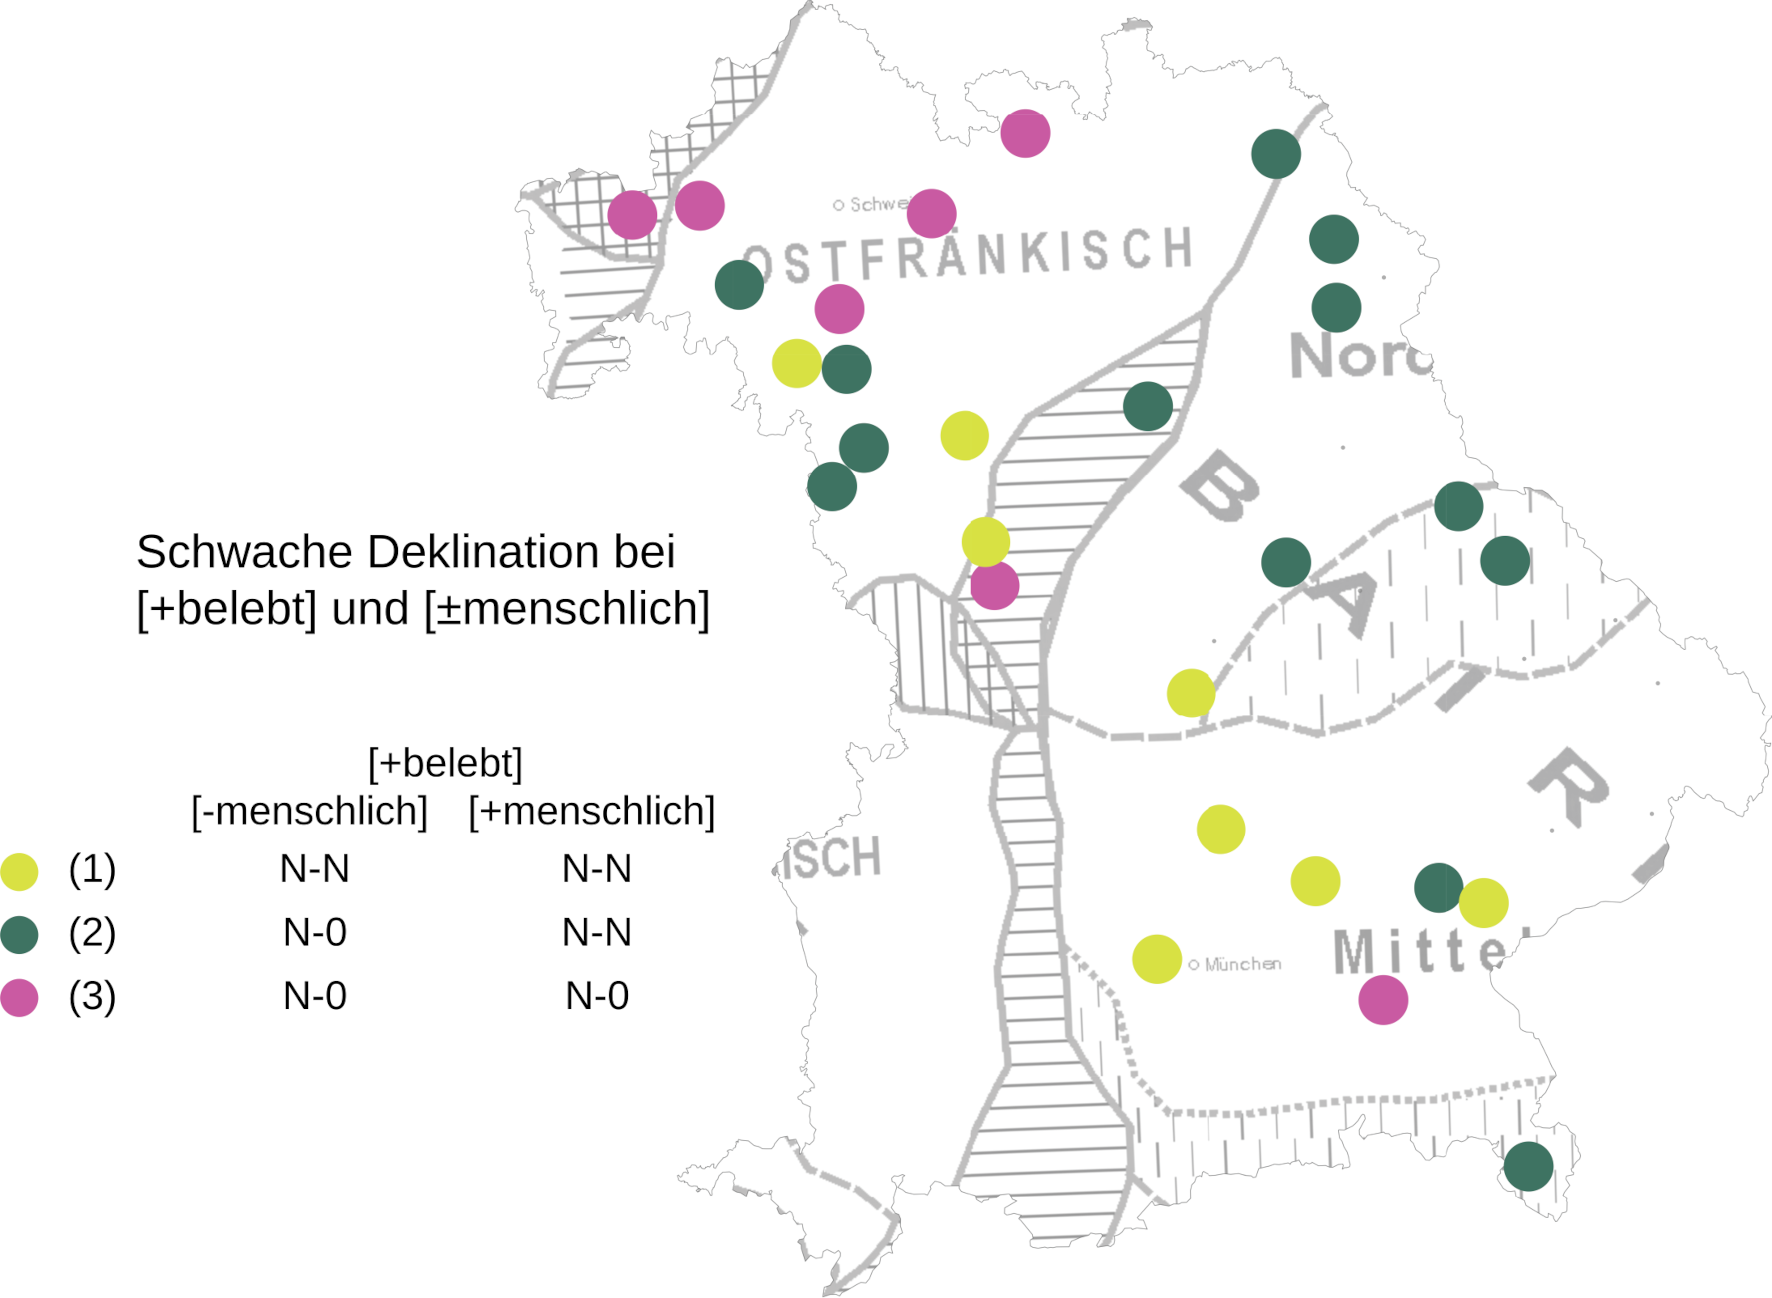
\includegraphics[width=\textwidth]{figures/Karte30.png}
\caption{Semantische Konditionierung der „schwachen“ Teilklassen N-N und N-0 durch die Distinktionen [+belebt] und [${\pm}$menschlich] bei den rezenten schwachen Maskulina ($n=124$)\protect\footnote{In den BSA-Daten ist nur ein schwaches Maskulinum mit dem Merkmal [+menschlich] in den obliquen Singularkasus erhoben worden (\textit{Bauer}); die Maskulina mit dem Merkmal [+belebt] und [$-$menschlich] sind \textit{Hase}, \textit{Hecht}, \textit{Karpfen}, \textit{Ochse}, \textit{Rabe} (\textit{Krack}), \textit{Ratte} und \textit{Spatz} (\textit{Sperk}).} }
\label{map:30}
\end{map}
\vfill\pagebreak

\mapref{map:30} zeigt, dass es auch in den Dialekten des UGs eine areale Distribution von drei Typen der Belebtheitsdistinktion gibt.\footnote{Bedingt durch die dünne Datenlage in den BSA-Teilprojekten des mittelbair. Dialektraums sind die kartierten Typen nur vorsichtig zu interpretieren (Voraussetzung war jeweils min. ein Beleg für die Distinktion [{${\pm}$}menschlich]. Teilweise finden sich keine Akkusativformen für Maskulina mit dem Merkmal [$-$menschlich], weshalb von einer Typisierung und Kartierung abgesehen wurde.}  Bei Typ (1), der vor allem im Nordbair. und im westlichen Ofr. zu finden ist, flektieren sämtliche belebte Maskulina nach dem Muster der schwachen Deklination (Deklinationsklasse N-N). Typ (2) beschreibt die Distinktion [${\pm}$menschlich] und damit eine Differenzierung des Belebtheitsmerkmals: Das Nasalsuffix der obliquen Singularkasus erscheint nur bei Maskulina mit dem Merkmal [+menschlich], Maskulina mit den Merkmalen [+belebt] und [$-$menschlich] weisen im Singular keine Kasusflexion auf (Deklinationsklasse N-0). Zudem ist der vollständige Abbau der Kasusflexion im Singular bei allen belebten Maskulina belegt; dieser Typ (3) ist vor allem im Unterofr. und im von \citet{Rowley1997} beschriebenen Coburger Raum zu finden (Tiefenbohrungspunkt Ahorn).

Dass bei Typ (1) das Merkmal [+belebt] die Deklinationsklassenzugehörigkeit steuert, ist in einem Teil der nordbair. Dialekte zu beobachten. Hier weist das his\-to\-ri\-sche \textit{n}{}-Maskulinum \textit{Karpfen} Nasalsuffix im obliquen Singularkasus auf, es liegt (vor der diachronen Folie) eine Art Doppelsuffigierung aus Nasalsuffix und vokalisch realisierter Reduktionssilbe mhd. -\textit{en} vor: Nom.Sg. \teuthoo{k,\_a.rpfA}{k͓ʰaͅrpfα} -- Akk.Sg. \teuthoo{An}{αn} \teuthoo{k,\_a.rpfAn}{k͓ʰaͅrpfαn} -- Nom.Pl. \teuthoo{k\_arpfAn}{kʰarpfαn} im nordbair. Kallmünz (vgl. Abschnitte~\ref{sec:7.2.1} und \ref{sec:7.2.2}). Das his\-to\-risch schwache, aber unbelebte Maskulinum \textit{Stecken} hingegen hat synkretische Formen im Singular: Nom.Sg. \teuthoo{s\#de.kA}{šdeͅkα} -- Akk.Sg. \teuthoo{s\#de.kA}{šdeͅkα} \teuthoo{s\#de.kA}{šdeͅkα} ‚einen Stecken (in den Boden) stecken‘ -- Nom.Pl. \teuthoo{s\#de.kAn}{šdeͅkαn} (Kallmünz). Im Nordbair. scheint es also tatsächlich das Merkmal [+belebt] zu sein, dass schwache Flexion im Singular und auch Deklinationsklassenwechsel steuert, etwa des historischen \textit{a}{}-Stamms \textit{Hecht}: Nom.Sg. \teuthoo{he4cd}{hẹXd} -- Akk.Sg. \teuthoo{An}{αn} \teuthoo{he4cdn@}{hẹXdn̥} -- Nom.Pl. \teuthoo{he4cdn@}{hẹXdn̥} im nordbair. Kallmünz (vgl. \citealt[§32.2]{Paul1968}).

\citet{DammelGillmann2014} haben für den „Sonderweg“ der historisch schwachen Maskulina argumentiert, dass die formale Distinktion zwischen Nom.Sg. und den obliquen Singularkasus durch das Belebtheitsmerkmal bedingt ist, da belebte Referenten sowohl als prototypisches Agens als auch als Patiens vorkommen; durch das schwache Flexionsmuster erfolgt eine formale Kodierung der unterschiedlichen syntaktischen Rollen.\footnote{Gleichwohl stellt Belebtheit nur einen Faktor dar, der aber nicht isoliert betrachtet werden dürfe, sondern im Zusammenhang mit dem gesamten Deklinationsklassensystem und dem morposyntaktischen Kontext der Nominalphrase (\citealt[212]{DammelGillmann2014}).} Belebtheitseffekte führen (vor dem Hintergrund des Relevanzprinzips) also zu einer „Relevanzerhöhung für Kasus“ (\citealt[211]{DammelGillmann2014}, ausführlicher \sectref{sec:5.2}). Gleichzeitig ist eine rezente Tendenz zum Abbau der schwachen Flexion im Singular zu beobachten (Gen./""Dat./""Akk.""Sg. \textit{Menschen} > \textit{Mensch} -- \textit{Menschen}). \citet[212]{DammelGillmann2014} folgern daraus, dass auch Belebtheit langfristig nicht vor dem Abbau des Kasusausdrucks am Substantiv schützt. Nach \citet{Köpcke2000a, Köpcke2002} ist allerdings nicht nur das Belebtheitsmerkmal zentral für das Schema der schwachen Maskulina, sondern erst die Kombination aus dem Merkmal [+menschlich] und dem phonologisch-prosodischen Merkmal finales Schwa (etwa in \textit{Bube}) ist ein verlässlicher Hinweis auf die schwache Deklination (siehe \sectref{sec:5.3.2}). Finales Schwa bei den Maskulina ist nach \citet[119]{Köpcke2000a} ein „Agentivitätsmarker“: Nur die schwache, nicht aber die starke Deklination weist ihn auf; Deflexion vollzieht sich ausgehend von der Peripherie (\textit{dem Mensch}), schließt aber nicht den prototypischen Kern des Schemas (mit finalem Schwa) ein \citep[105]{Köpcke2002}.

Zumindest für die nordbair. Dialekte muss für das Schema der schwachen Maskulina angenommen werden, dass phonologische Merkmale weniger zentral sind: Auch ein zweisilbiges Maskulinum wie \textit{Karpfen} weist schwache Flexion auf. Hier ist der zentrale Konditionierungsfaktor das semantische Merkmal [${\pm}$belebt]. Da finales Schwa als „formales Korrelat“ (\citealt[119]{Köpcke2000a}) des semantischen Merkmals [+menschlich] in den oobd. Dialekten apokopiert ist, scheint die Semantik neben Genus der einzige (verbleibende) Hinweisgeber auf die schwache Deklination zu sein -- zumindest in jenen Dialekten, die eine distinkte Kasusform im Singularparadigma erhalten haben.

Grundsätzlich wären hier weitere, systematisch erhobene Daten wünschenswert. Denn auch in den Dialekten mit Belebtheitskonditionierung des Typs (1) und (2) weisen nicht alle belebten Maskulina Nasalsuffigierung in den obliquen Singularkasus auf; vor allem \textit{Spatz} und daneben auch \textit{Ratte} und -- als Einzelbeleg im ofr. Gebsattel -- \textit{Ochse} flektieren nach dem Muster N-0 (siehe hierzu auch \sectref{sec:7.2.2}). Hier braucht es weitere Daten, um eine mögliche Abstufung des semantischen Merkmals Belebtheit abbilden oder den Abbau der Kasusmarkierung auf mögliche Frequenzeffekte zurückführen zu können.

In den untersuchten Dialekten finden sich weitere Fälle von Deklinationsklassenwechsel in das Pluralverfahren mit Nasalsuffix: bei dem historischen \textit{i}{}-Stamm \textit{Fuchs} im südlichen Nordbair. und im Mittelbair., \textit{Hecht} im Nordbair. und Ofr. sowie im Ofr. bei den \textit{a}{}-Stämmen \textit{Hund}, \textit{Knecht} und dem \textit{i-}Stamm \textit{Wirt}.\footnote{\citet[§20--21]{Micko-Repp1933} führt daneben noch den Wechsel der historisch starken Maskulina \textit{Wolf}, \textit{Bär}, \textit{Eber}, \textit{Hengst} und \textit{Krebs} in die schwache Flexion an.} Bei den Maskulina ist die Pluralmarkierung durch Nasalsuffix dialektübergreifend mit dem semantischen Merkmal [+belebt] assoziiert.\footnote{Ob diese Lexeme auch in die schwache Kasusflexion im Singular gewechselt sind, lässt sich nur für \textit{Hecht} sagen, da die übrigen Maskulina nicht in den obliquen Kasus erhoben wurden: \textit{Hecht} flektiert nur im Nordbair. (inkl. Übergangsgebiet) nach dem Muster der schwachen Deklination (Klasse N-N), in den übrigen (ofr.) Dialekt erfolgte Wechsel in die Deklinationsklasse N-0.} Gleichzeitig bewahren andere Maskulina mit belebtem oder menschlichem Denotat die historische Deklinationsklasse, etwa die \textit{i}{}-Stämme \textit{Fisch} und \textit{Frosch}.

Bei den Feminina ist \textit{n}{}-Plural bei der großen Gruppe der historischen \textit{n}{}- und \textit{ô}{}-Deklination und nicht exklusiv bei belebtem Denotat zu finden. Allerdings findet eine semantische Konditionierung von Nullplural vs. Nasalsuffix bei Feminina mit dem Merkmal [+belebt] entlang der Individuierungshierarchie statt: Belebte Denotate, die individuell und nicht als in Mengen oder Scharen vorkommend wahrgenommen werden, haben eine distinkte Pluralform mit Nasalsuffix, etwa der historische n-Stamm \textit{Katze} (Typ \teuthoo{katS}{katʃ} -- \teuthoo{katSn}{katʃn}) oder die Klassenwechsler \textit{Geiß} (Typ \teuthoo{ga2s}{ɡās} -- \teuthoo{ga2sn}{ɡāsn}) und \textit{Magd} (Typ \teuthoo{ma2d}{mād} -- \teuthoo{ma2dn}{mādn}) im Ofr.

Im südlichen Nordbair. und in Teilen des Mittelbair. konditioniert das semantische Merkmal [+verwandt] in Kombination mit der prosodisch-phonotaktischen Inputbedingung einer Tiefschwa-Reduktionssilbe schwache Flexion im Singular: bei den Feminina mit einer distinkten Dativ-Singular-Form (Typ Nom./Akk.Sg. \teuthoo{mutA}{mutα} -- Dat.Sg. \teuthoo{mutAn}{mutαn} -- Pl. \teuthoo{mutAn}{mutαn}), bei den maskulinen Verwandtschaftsbezeichnungen mit Nasalsuffix in den obliquen Singularkasus (Akk./Dat.Sg. \teuthoo{våtAn}{v{\burgeroalpha}tαn}, vgl. Abschnitte~\ref{sec:7.2.2} und \ref{sec:8.3.3.1}). Verwandtschaftsbezeichnungen sind auf \citegen{Corbett2000} Belebtheitshierarchie noch näher am Sprecher angeordnet, weshalb die semantische Konditionierung dieses spezifischen Flexionsmusters durch die -- in \citegen{Comrie1981} Terminologie -- höhere Salienz erklärt werden kann.

\subsection{Formale Konditionierung}\label{sec:8.3.3}
\begin{sloppypar}
Die in \sectref{sec:3.2} vorgestellten Studien zu Konditionierungswandel haben ergeben, dass diachron ein Abbau von Komplexität der Konditionierung von Deklinationsklassen erfolgt, da zu dem primären Konditionierungsprinzip Genus formale Konditionierungsfaktoren und die in \sectref{sec:8.3.2} behandelte semantische Konditionierung hinzukommen (vgl. \citealt{DammelKürschner2008}, \citealt{Kürschner2008a}). Diese Formalisierung der Konditionierung ist auch in den untersuchten Dialekten zu beobachten. Es sind vor allem prosodische und phonotaktische Steuerungsprinzipien, die diachron zu einer Reorganisation der Klassen führen und auch synchron die Distribution der Pluralallomorphe in einzelnen Dialekten steuern. Die zu beobachtenden prosodischen und phonotaktischen Konditionierungsprinzipien sind spezifisch für Teile der untersuchten bair. Dialekte. Die formale Konditionierung bedingt hier additive Pluralmarkierung (gegenüber Null in Dialekten ohne diese Kodierung) oder steuert die Distribution der additiven Allomorphe.
\end{sloppypar}

Formale Konditionierung ist, wie \citet[33]{Harnisch1987} herausstreicht, auch kog"-ni"-tiv vorteilhaft, da phonologische Muster es „erlauben, lernpsychologisch (mnemotechnisch) gesehen, Voraussagen über das Wie der morphologischen Kodierung“ zu treffen. Damit ist für einige bair. Dialekte eine Zweiteilung der Formenbildung zu beobachten: eine Formalisierung der Konditionierung der additiven Markierung einerseits und anderseits ein hohes Maß an Lexikalisierung morphophonologischer Alternationen, die zwar mnemotechnisch aufwändiger sind, dafür aber einen direkten Zugriff auf die gesamte Form erlauben (vgl. \citealt[59]{Harnisch1990} und \sectref{sec:5.1}).

\subsubsection{Prosodische Konditionierung}
\label{sec:8.3.3.1}
Die dialektraumspezifische Distribution von additiven und Nullpluralen in den ofr. und bair. Dialekten des UGs ist das Ergebnis wiederum dialektraumspezifischer prosodischer Input- und Outputkonditionierung, d.\,h. Konditionierung, die entweder die Form und strukturelle Eigenschaften der Basisform oder des Flexionsprodukts betrifft. Im südlichen Nordbair. und in Teilen des Mittelbair. sind genusübergreifend Formen von prosodischer Inputkonditionierung bei zweisilbigen Singularstämmen auf Reduktionssilbe zu finden, die den Plural regelmäßig additiv markieren; im Ofr. und im nördlichen Nordbair. hingegen erscheint Nullplural. Genusspezifisch ist dabei allerdings die Spezifikation der Inputbedingung, da neben der prosodischen Struktur die Form der Reduktionssilbe bei den Genera unterschiedlich steuernd wirkt. 

Regelmäßig bei allen Genera erfolgt die additive Markierung mit Nasalsuffix bei \textit{el}-Reduktionssilbe (realisiert als [l̥] oder vokalisiert zu [i] oder [e] im Mittelbair.). \mapref{map:31} zeigt, dass additive Pluralmarkierung durch Nasalsuffix bei Feminina in weiten Teilen des UGs verbreitet ist (ausgenommen sind das nördliche Nordbair. und der westliche Vokalisierungsstreifen des Ofr.). Bei Maskulina und Neutra hingegen ist diese Form der Markierung vor allem im südlichen Nordbair. und vereinzelt im Mittelbair. belegt. Bei den Neutra handelt es sich ausschließlich um Diminutiva (siehe \sectref{sec:8.3.4} zur diatopisch variierenden Pluralmarkierung der Diminutiva).\footnote{Die Schwankung der absoluten Zahlen von Nasalsuffigierungen nach \textit{el}{}-Reduktionssilbe bei Neutra ergibt sich vor allem auch aus Zusammensetzung der Daten. Im mittelbair.-südbair. Ramsau etwa sind auch da Diminutivformen belegt, wo im BSA-Fragebuch Simplizia erhoben wurden. In den übrigen Ortsdialekten sind hingegen nur dann Diminutiva in den Daten zu finden, wenn diese systematisch abgefragt wurden.} In den ofr. Dialekten, die Nasalsuffix-Plural bei Feminina auf -\textit{el} haben, weisen die Maskulina Nullplural auf. Daneben ist in einem Teil des ofr.-nordbair. Raums Nasalsuffigierung bei \textit{el}{}-Reduktionssilbe laut \citet[169]{Rowley1997} sogar „grundsätzlich ausgeschlossen“, d.\,h. auch bei den Feminina \textit{Wurzel}, \textit{Gabel} usw. (siehe auch \citealt[148]{Rowley1997}).



\begin{map}
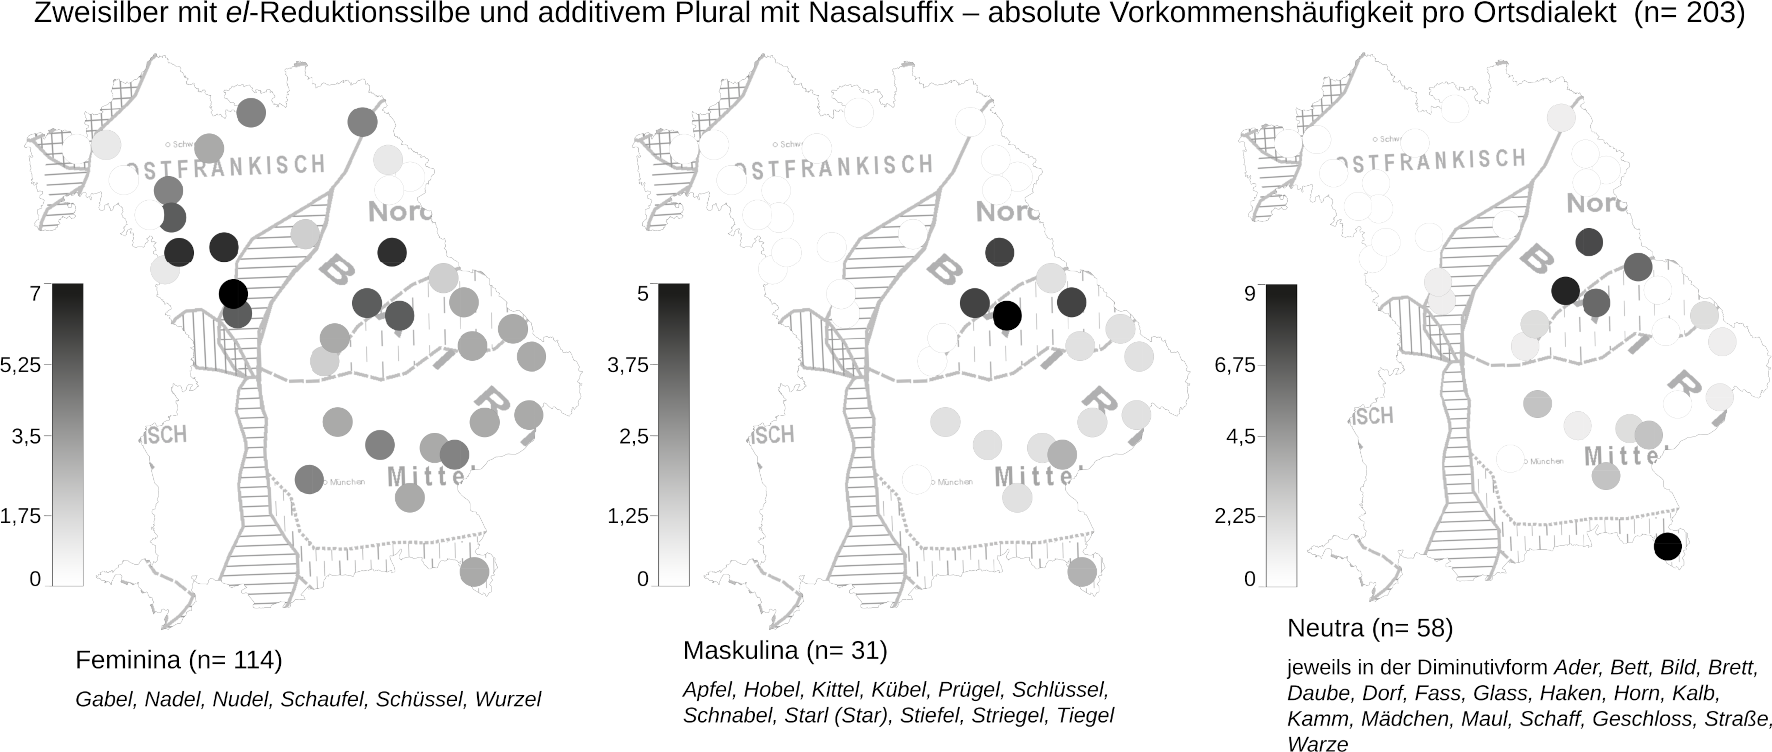
\includegraphics[width=\textwidth]{figures/Karte31.png}
\caption{Prosodische Inputkonditionierung bei \textit{el}{}-Reduktionssilbe}
\label{map:31}
\end{map}

Diversen dialektologisch-grammatischen Darstellungen zufolge erscheint die \textit{n}{}-Suffigierung bei Maskulina nur dann, wenn kein Umlaut-Plural vorliegt (vgl. \citealt[158]{Rowley1997}, \citealt[421]{Schirmunski1962}, \citealt[§801]{Schmeller1821}, \citealt[§11e]{Weitzenböck1942}). Im südlichen Nordbair. (Tiefenbohrungspunkt Bernhardswald) finden sich indes Belege historischer \textit{i}{}-Maskulina mit \textit{el}{}-Reduktionssilbe, die auch Umlautplural aufweisen (Pl. \teuthoo{ds\#na\$wl°@n@}{dšna̤wl̥̑n̥} ‚Schnäbel‘, \teuthoo{epfl°@n@}{epf‌l̥̑n̥} ‚Äpfel‘, siehe \sectref{sec:8.2.1}). Hier hat die prosodische Input-Konditionierung zu kumulativer Markierung geführt. \citet[153]{Rowley1997} zufolge sind die additiven Pluralformen mit Nasalsuffix bei den Maskulina fakultative Markierungen, die bei fehlender Disambiguierung der Numerusinformation im syntaktischen Kontext erfolgt (vgl. \citealt[158]{Rowley1997} sowie \sectref{sec:9.2}). Auch \citet[421]{Schirmunski1962} nennt Beispiele für ein Fehlen des \textit{n}{}-Suffixes bei vorausgehendem Zahlwort: \teuthoo{s\#lisln}{šlisln} ‚Schlüssel‘, aber \teuthoo{tswaI2\textsuperscript{n}}{tswaı̄\textsuperscript{n}} \teuthoo{s\#lisl}{šlisl} ‚zwei Schlüssel‘.\footnote{Dies können die eigenen Daten weder bestätigen noch widerlegen, da es sich um isolierte Abfrage-Items handelt und keine Aussagen über semantisch-pragmatische Kontextbedingungen von distinkten oder synkretischen Formen gemacht werden können.}



\begin{map}
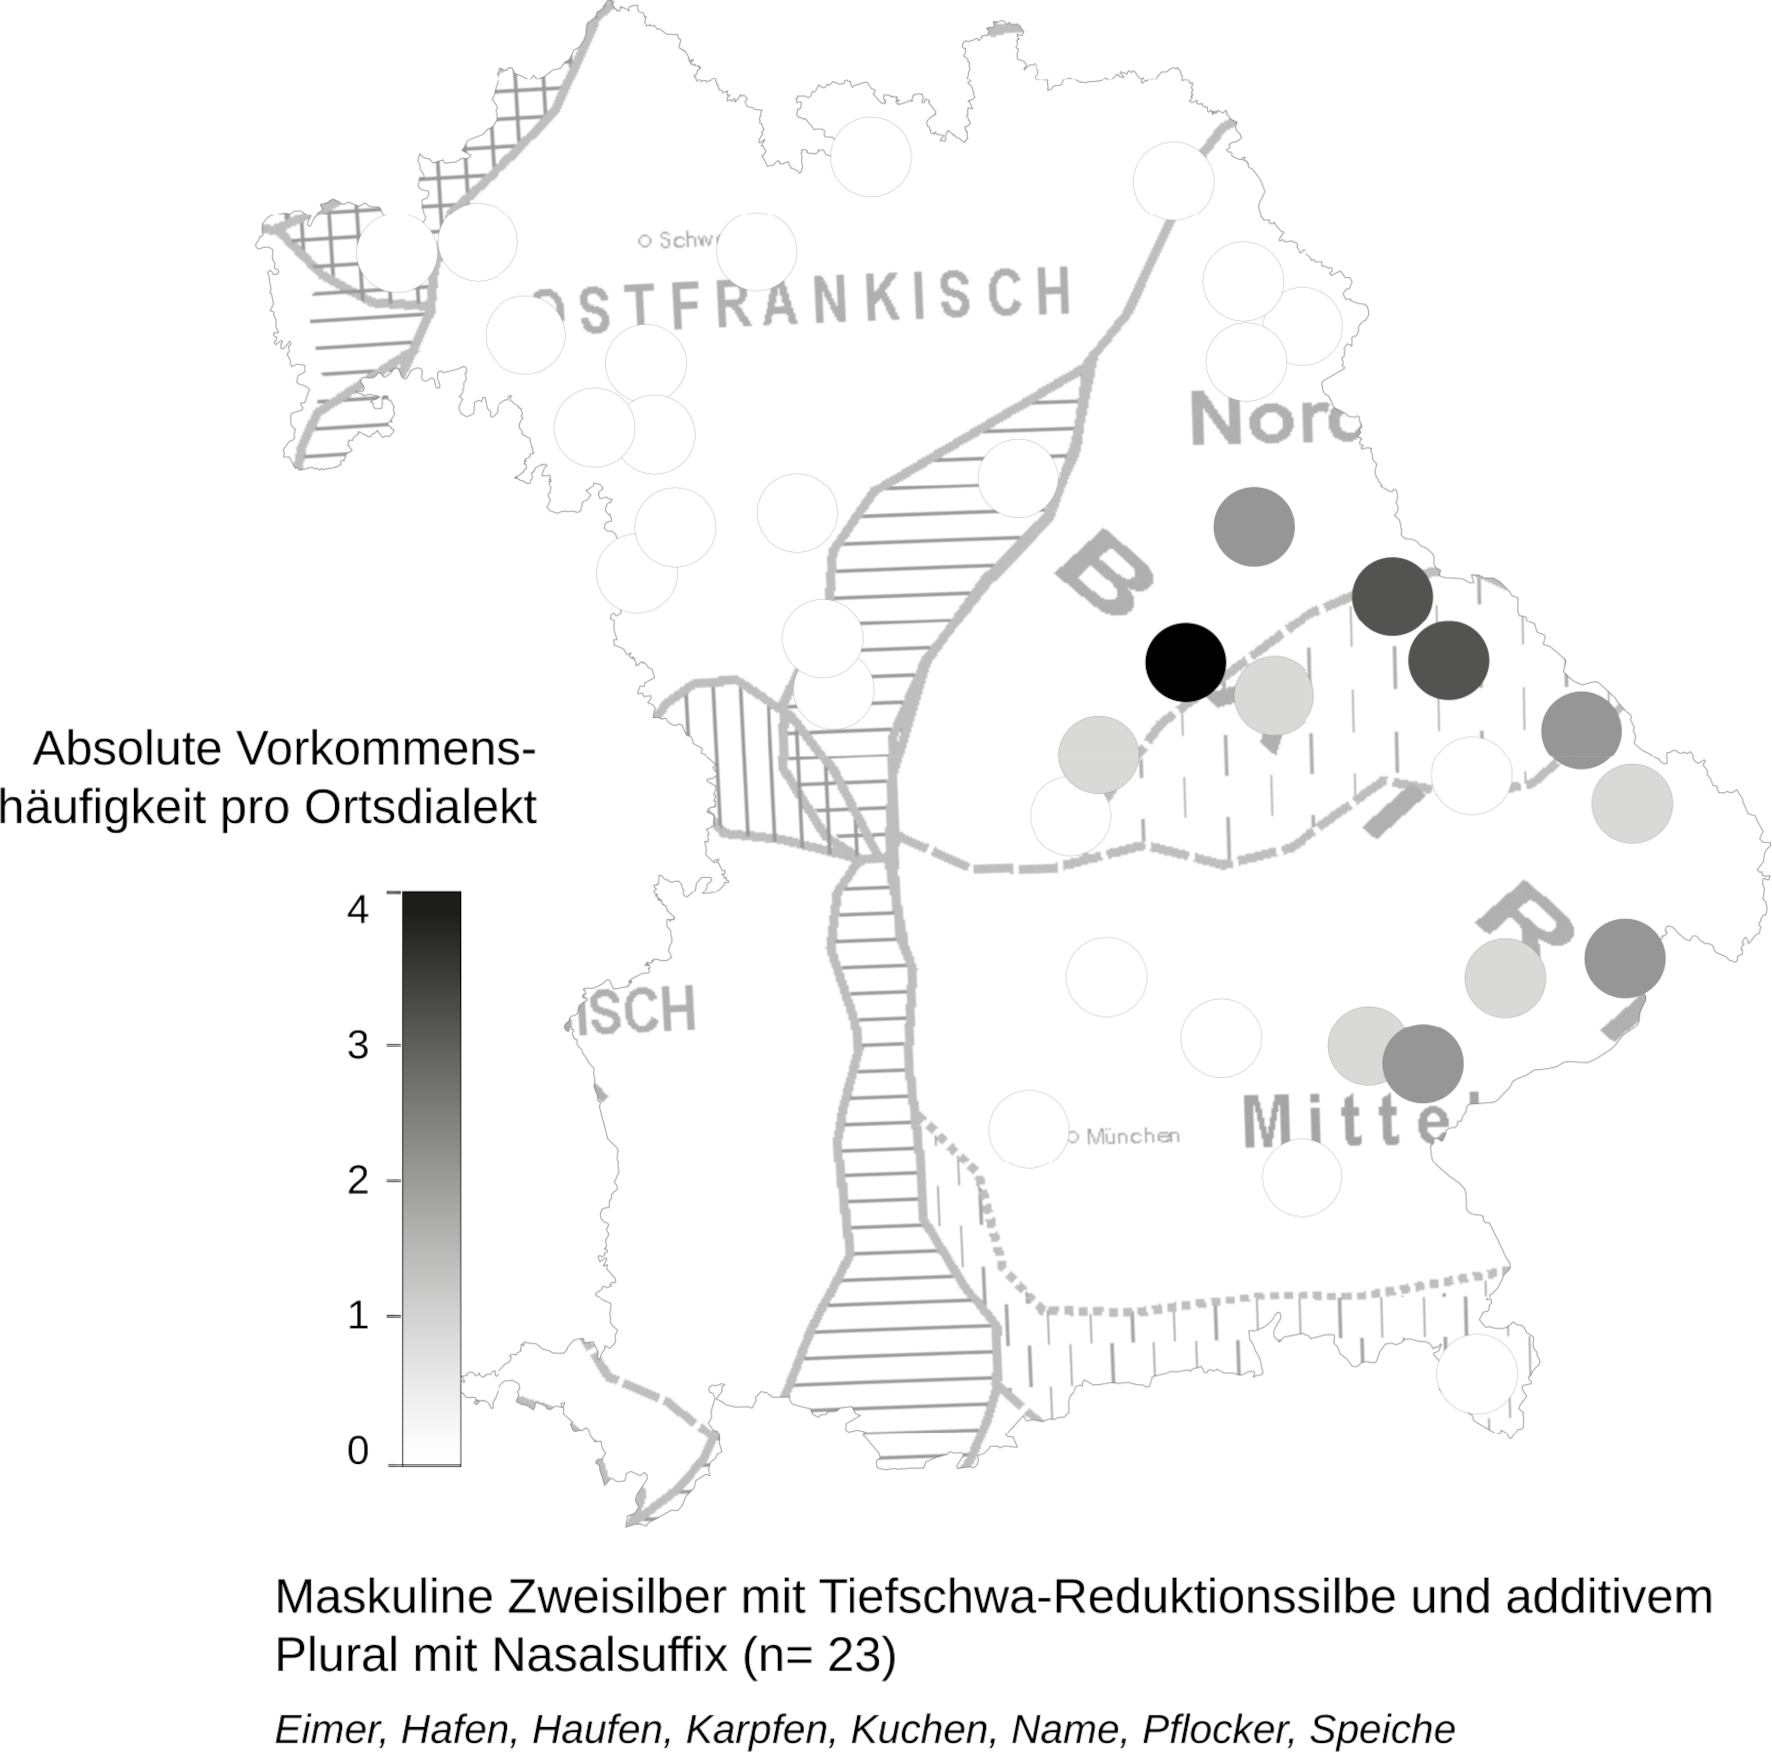
\includegraphics[width=\textwidth]{figures/Karte32.png}
  \caption{Prosodische Inputkonditionierung bei zweisilbigen Maskulina mit Tiefschwa-Reduktionssilbe}
  \label{map:32}
\end{map}

Eine weitere Form der Inputkonditionierung besteht aus Zweisilbigkeit und Tiefschwa-Reduktionssilbe für Feminina und Maskulina. Methodisch stellt sich auch hier die Frage, ob Tiefschwa als heteromorphische Variante für mhd. \mbox{-\textit{er}} und -\textit{en} klassifiziert wird oder einen eigenen Typus darstellt (siehe die Diskussion in \sectref{sec:7.1.1.1} sowie \citealt[128, 166--168]{Rowley1997}). Unter Berücksichtigung der arealen Distribution der Pluralformen und der diachronen Folie ist es bei den Feminina von Vorteil, zunächst die Differenzierung von mhd. -\textit{er} und -\textit{en} auch für die rezenten Dialekte beizubehalten, da sie aufzeigt, inwiefern die Inputkonditionierung einer Tiefschwa-Reduktionssilbe tatsächlich dialektraumspezifisch ist. Pluralformen mit Nasalsuffix (Typ \teuthoo{biEkA}{biəkα} -- \teuthoo{biEkAn}{biəkαn} ‚Birke‘), bei denen Tiefschwa die phonotaktisch bedingte Entsprechung der Reduktionssilbe mhd. -\textit{en} im Nom.Sg. ist, finden sich im südlichen Nordbair. und im Mittelbair. (\mapref{map:4} und \mapref{map:29}). Die Markierung mit Nasalsuffix bei Reduktionssilbe mhd. \mbox{-\textit{er}} (Typ \teuthoo{kha.mA}{khaͅmα} -- \teuthoo{kha.mAn}{khaͅmαn} ‚Kammer‘) ist indes in allen Dialekten des UGs belegt und entspricht der historischen Deklination (fem. \textit{ô}, ebenso bei \textit{Ader} und \textit{Feder}). Für das Bair. ist damit bei den Feminina eine Inputkonditionierung aus Zweisilbigkeit und Tiefschwa-Reduktionssilbe anzunehmen; hier werden mhd. \mbox{-\textit{er}} und -\textit{en} in der Realisierung als -\textit{α} in den rezenten Flexionssystemen nicht differenziert. Auch die semantisch konditionierte Deklinationsklasse „enge Verwandtschaftsbezeichnungen“, die \citet[137]{Rowley1997} für Teile des Nordbair. anführt und die im Paradigma Nasalsuffigierung aufweist, ist nicht nur durch das semantische Merkmal, sondern auch durch die prosodische Inputkonditionierung einer Tiefschwa-Reduktionssilbe bedingt (vgl. \citealt[170]{Rowley1997}, siehe Abschnitte~\ref{sec:7.2.2} und \ref{sec:8.3.2.2}).


Bei den Maskulina erfolgt im südlichen Nordbair. und im Mittelbair. die additive Pluralmarkierung regelmäßig bei vokalisch realisiertem Nasalsuffix (Typ \teuthoo{hoafA}{hoafα} -- \teuthoo{hoafAn}{hoafαn} ‚Haufen‘) und vereinzelt auch bei \textit{er}{}-Reduktionssilbe, etwa bei \teuthoo{e<.mA}{êͅmα} -- \teuthoo{e<.mAn}{êͅmαn} ‚Eimer‘ (nordbair.-mittelbair. Blaibach) oder bei \teuthoo{gho2da}{ɡhōda} -- \teuthoo{gho2dan}{ɡhōdan} ‚Kater‘, \teuthoo{ghe2va}{ɡhēva} -- \teuthoo{ghe2van}{ɡhēvan} ‚Käfer‘ (\citealt[128 und 154]{Rowley1997}, vgl. \citealt[§38]{Kollmer1985}). Hier liegt -- der phonetischen Form des Singularstammes entsprechend -- ebenfalls eine konditionierende Inputbedingung zweisilbiger Singularstamm mit Tiefschwa-Reduktionssilbe vor. Laut \citet[153]{Rowley1997} ist die additive Markierung mit Nasalsuffix bei den Maskulina auf Tiefschwa-Reduktionssilbe (wie auch bei Maskulina auf -\textit{el}) fakultativ, \citet[421]{Schirmunski1962} beschreibt sie als „weniger konsequent“ als bei \textit{el}{}-Reduktionssilbe.


Doch auch wenn die additive Markierung bei den Maskulina kein sehr frequentes Phänomen ist (vgl. \mapref{map:32}), so lassen die Belege doch den Schluss zu, dass Nasalsuffigierung (und damit ein Deklinationsklassenwechsel) dann realisiert wird, wenn keine andere Form der Numerusdistinktion vorliegt. Der historische \textit{i}{}-Stamm \textit{Hafen} etwa wird im Bair. mit Umlautplural markiert (neben zahlreichen Markiertheitsumkehrungen); nur im mittelbair. Grafenau liegt keine Vokalalternation vor, es erscheint Nasalsuffigierung (\teuthoo{ho.<v5A}{hôͅv̩α} -- \teuthoo{ho.<vAn}{hôͅvαn}). Dass die beschriebene Inputbedingung in diesem Teil des Bair. einen produktiven prosodischen Steuerungsfaktor darstellt, zeigen zudem vereinzelte Belege, die nicht auf alte Reduktionssilben zurückgehen. Bei Komposita mit dem Zweitglied \textit{{}-tag} wird im UG teilweise die Nebenakzentsilbe reduziert (z.\,B. ofr. \textit{doog} > \mbox{-\textit{ic}}, \citealt[338]{Schmidt1905}).\footnote{Vgl. \citet[22--23]{Köhler1934}, \citet[Karte 12]{Roth1940}, \citet[15]{Schießl1909}.} Infolge der Reduktion erscheint im bair. Teil des UGs für das Kompositum \textit{Werktag} die prosodische Struktur eines Zweisilbers auf Tiefschwa-Reduktionssilbe. Im nordbair.-mittelbair. Übergangsgebiet sind der Inputkonditionierung entsprechend additive Pluralformen mit Nasalsuffix belegt: \teuthoo{we.2AdA}{wēͅαdα} -- \teuthoo{we.2AdAn}{wēͅαdαn} (Zwiesel) und \teuthoo{weEdA}{weədα} -- \teuthoo{weEdAn}{weədαn} (Bern\-hards\-wald, der Simplex \textit{Tag} hat dagegen Null- oder Umlautplural).\footnote{\citet[422]{Schirmunski1962} führt daneben den Beleg \teuthoo{fraI2dA}{fraı̄dα} -- \teuthoo{fraI2dAn}{fraı̄dαn} ‚Freitag‘ an.}


Für jene Feminina, die das Nasalflexiv der obliquen Kasus im Nom.Sg. aufweisen, kann im Bair. eine prosodische und phonotaktische Inputkonditionierung angenommen werden (zur Singularstammbildung siehe Abschnitte~\ref{sec:7.1.3.1} und \ref{sec:8.3.1.3}). Die prosodische Struktur ist auch hier zweisilbig, die Reduktionssilbe mhd. -\textit{en} wird als Nasal (Typ \teuthoo{das\#n}{dašn} ‚Tasche‘) oder vokalisch (Typ \teuthoo{biEkA}{biəkα} ‚Birke‘) in Abhängigkeit vom Stammauslaut realisiert. Die Form des Suffixes, das bei der additiven Markierung dieser zweisilbigen Feminina mit \textit{en}-Reduktionssilbe erscheint, ist phonotaktisch konditioniert: Nach Nasal erscheint \textit{α}{}-Suffix (Typ \teuthoo{das\#n}{dašn} -- \teuthoo{das\#nA}{dašnα}), nach Tiefschwa Nasalsuffix (Typ \teuthoo{biEkA}{biəkα} -- \teuthoo{biEkAn}{biəkαn}, vgl. \sectref{sec:8.3.3.2}). \figref{fig:15} illustriert, dass eben diese Inputstruktur auf Tief\-schwa-Re\-duk\-tions\-sil\-be das Muster für die mask. Deklinationsklassenwechsel bildet. Mit Blick auf die Interdependenz der Konditionierungsprinzipien ist bemerkenswert, dass in Nabburg im mittleren Nordbair. die additive Markierung nach Tiefschwa-, nicht aber nach Nasalsuffix im Nom.Sg. belegt ist (vgl. \mapref{map:4} und \mapref{map:29}). Die zweisilbige Inputstruktur ist damit eine notwendige, aber keine hinreichende Bedingung; die phonotaktische Inputbedingung (hier die Form der Reduktionssilbe) wirkt gleichermaßen steuernd (additive Markierung erfolgt bei Tief\-schwa-Re\-duk\-tions\-sil\-be, nicht aber nach Nasal).



\begin{figure}
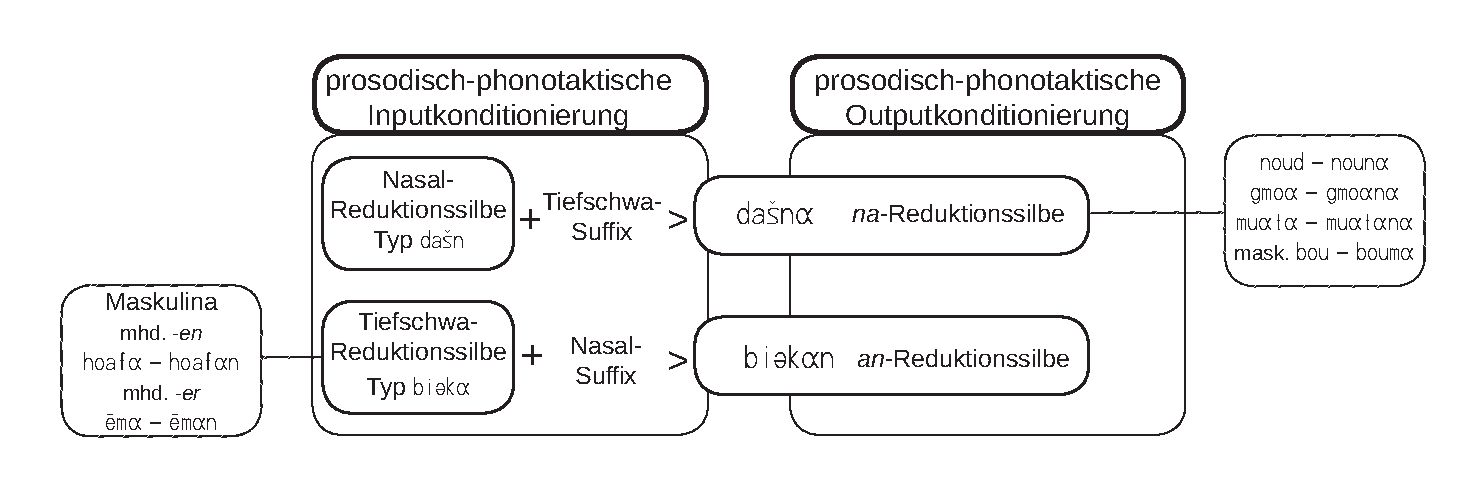
\includegraphics[width=\textwidth]{figures/Outputkonditionierung.pdf}
\caption{Input- und Outputkonditionierung der Feminina}
\label{fig:15}
\end{figure}

Neben diesen Formen der Inputkonditionierung ist in den bair. Dialekten auch eine prosodische Konditionierung auf Basis des Outputs für fem. Pluralformen festzustellen. Es handelt sich um zwei präferierte Outputstrukturen, die in den Dialekten des südlichen Nordbair. und im Mittelbair. parallel vorkommen und in Kombination mit phonotaktischer Konditionierung beschrieben werden müssen. Ein Typus besteht darin, dass Pluralformen präferiert zweisilbig sind und auf Reduktionssilbe {-\textit{αn}} enden, er findet sich bei verschiedenen Singularstammformen und als Ergebnis folgender additiver Verfahren:

\begin{itemize}\sloppy
\item „Doppelsuffigierung“ bei Feminina mit als Tiefschwa realisiertem Nasalsuffix in der Nominativ-Singular-Form (Typ \teuthoo{biEkA}{biəkα} -- \teuthoo{biEkAn}{biəkαn} ‚Birke‘)
\item Suffixalternation \textit{{}-n} > -\textit{αn} bei Feminina mit Nasalsuffix in der Nominativ-Singular-Form (Typ \teuthoo{biEkN}{biəkŋ} -- \teuthoo{biEkAn}{biəkαn})
\item Additive Markierung mit \textit{αn}{}-Suffix von einsilbigen, meist apokopierten Singularstämmen auf Plosiv (Typ \teuthoo{biEk}{biək} -- \teuthoo{biEkAn}{biəkαn}) oder mit vokalischem Auslaut (\teuthoo{vrau}{vrau} -- \teuthoo{vrauAn}{vrauαn} ‚Frau‘, vgl. \citealt[153]{Rowley1997})
\item Additive Markierung mit \textit{n}{}-Suffix von Simplizia mit Tief\-schwa-""Re\-duk\-tions\-sil\-be (Typ \teuthoo{o2dA}{ōdα} -- \teuthoo{o2dAn}{ōdαn} ‚Ader‘)
\end{itemize}

Die zweite präferierte Outputstruktur endet auf Reduktionssilbe {-\textit{nα}}. Dieser Bedingung entsprechen die \textit{n}{}-erweiterte Feminina des Typs \teuthoo{das\#n}{dašn} -- \teuthoo{das\#nA}{dašnα} sowie auf Nasal auslautende Simplizia mit \textit{α}{}-Suffix (Typ \teuthoo{diAn}{diαn} -- \teuthoo{diAnA}{diαnα} ‚Dirn‘). Daneben finden sich Klassenwechsel von Feminina, die his"=to"=risch keinen Plural mit Nasalsuffix bildeten, etwa die historischen \textit{i}{}-Stämme \teuthoo{nôo(+u(+d5}{n{\aufstrih}õ\klammerobenpost{}ũ\klammerobenpost{}d̩} -- \teuthoo{nôo(+u(+nA}{n{\aufstrih}õ\klammerobenpost{}ũ\klammerobenpost{}nα} ‚Naht‘ (nordbair. Oberdolling) oder \teuthoo{d5i“4a}{d̩ị̄a} -- \teuthoo{d5i“4AnA}{d̩ị̄αnα} ‚Tür‘ (mittelbair. Kirchensur) sowie der kontrahierte Stamm \teuthoo{gmo>+A+}{ɡmỗα̃} -- \teuthoo{gmo2A2nA}{ɡmōᾱnα} ‚Gemeinde‘ (mittelbair.-südbair. Ramsau, vgl. 	\tabref{tab:37} und \citealt[160]{Rowley1997}). In diesen Fällen war Deklinationsklassenwechsel in eine Pluralform auf Na"=sal+""Tief"=schwa durch die Outputbedingung gesteuert. Bemerkenswert mit Blick auf die Herausbildung des nhd. Systems, das durch die Outputbedingung eines (idealiter trochäischen) Plurals auf Reduktionssilbe geprägt ist, sind dabei dreisilbige Pluralformen, die auf zwei Reduktionssilben schließen: \teuthoo{bmuAtA}{bmuαtα} -- \teuthoo{muAdAnA}{muαdαnα} ‚Mutter‘ (nordbair.-mittelbair. Blaibach), \teuthoo{A}{α} \teuthoo{d5e."+nA}{d̩ẽ̄ͅnα} -- \teuthoo{de.>+nAne4}{dễͅnαnẹ} ‚Tanne‘ (mittelbair. Grafenau), \teuthoo{gbma4end5e4}{ɡbmạend̩ẹ} -- \teuthoo{gbma4end5e4NA}{ɡbmạend̩ẹŋα} ‚Gemeinde‘ (nordbair.-mittelbair. Blaibach) oder -- mit vokalisierter \textit{el}{}-Reduktionssibe -- \teuthoo{go42we4}{ɡọ̄wẹ} -- \teuthoo{go42we4nA}{ɡọ̄wẹnα} ‚Gabel‘ (mittelbair. Nöham, vgl. \citealt[128]{SNiB7}). Um die Outputbedingung Nasal+Tiefschwa zu erfüllen, werden hier auch Daktylen akzeptiert.


Damit zeigen die Daten, dass die beiden Outputstrukturen unabhängig von der phonotaktischen Bedingung steuernd wirken, auch wenn die Distribution der Allomorphe Nasal- oder Tiefschwa-Suffix primär phonotaktisch durch den Stammauslaut oder die Form der Reduktionssilbe konditioniert ist. Die Outputbedingung kann die vereinzelt belegten Suffixalternationen \textit{{}-n} > {}-\textit{αn} erklären oder dass bei assimiliertem Nasalsuffix in der Nominativ-Singular-Form eine „Doppelsuffigierung“ mit \textit{αn}{}-Suffix und nicht mit \textit{α}{}-Suffix erfolgt (z.\,B. \teuthoo{s\#d5u4<m}{šd̩ụ̂m} -- \teuthoo{s\#5d\%u.mAn}{š̩d͈uͅmαn} ‚Stube‘ im mittelbair. Inning am Holz vs. \teuthoo{s\#tu.m}{štuͅm} -- \teuthoo{s\#tu.mA}{štuͅmα} im mittelbair. Kirchensur). Hier scheint es eine Art Übergangsbereich zwischen beiden Outputbedingungen oder vielmehr ein gewisses Maß an Varianz in der Formenbildung zu geben. Auch \citet[153]{Rowley1997} gibt an, dass die Suffigierung mit \textit{αn}{}-Suffix nach Nasal -- anders als nach Plosiv oder vokalischem Stammauslaut -- „nicht zwingend“ erfolgt, es finden sich auch Formen mit Tiefschwa-Suffix. Daneben finden sich etwa im mittelbair. Grafenau die Varianten \teuthoo{d5e."+nA}{d̩ẽ̄ͅnα} -- \teuthoo{de.>+nAn}{dễͅnαn} und \teuthoo{de.>+nAne4}{dễͅnαnẹ} als Pluralformen für ‚Tanne‘. Gleichzeitig besteht Varianz zwischen synkretischen und distinkten Formen, etwa bei \teuthoo{wo42xA}{wọ̄xα} -- \teuthoo{wo42xA}{wọ̄xα} neben \teuthoo{wo42xAnA}{wọ̄xαnα} ‚Woche‘ (nordbair.-mittelbair. Blaibach).

\subsubsection{Phonotaktische Konditionierung}
\label{sec:8.3.3.2}
Phonotaktische Konditionierung ist in den untersuchten Dialekten stark an spezifische phonologische Entwicklungen im Auslaut des Stammes geknüpft. Es geht im Folgenden daher weniger um allgemeine Prinzipien der Auslautkonditionierung in den Dialekten, sondern anhand zweier Phänomene wird die Interdependenz von phonologischem und morphologischem Wandel aufgezeigt. Historisch hat so die mittelbair. Liquidvokalisierung zu einer Reorganisation von Pluralallomorphie und damit der Klassenzugehörigkeit geführt. In den bair. Dialekten ist damit eine dialektraumspezifische Form der phonotaktischen Konditionierung zu finden, die im Korpus Lexeme mit mhd. {\textit{l}} im Auslaut und das stammaffizierende Verfahren Umlaut betrifft.

Die Liquidenvokalisierung ist ein Teilphänomen der mittelbair. Konsonantenschwächung (\citealt[49c6]{Kranzmayer1956}, vgl. \citealt[419]{Rowley1990b}). Vokalisierung wird nach \citet[1111]{Haas1983} als diachrone oder synchrone Lautveränderung definiert, durch die ein Konsonant vokalisch realisiert wird, beispielsweise das postvokalische /l/ in mittelbair. \teuthoo{woid}{woid} vs. ofr./nordbair. \teuthoo{wold}{wold} ‚Wald‘ und das intervokalische /l/ in mittelbair. \teuthoo{keiA}{keiα} vs. ofr./nordbair. \teuthoo{kela}{kela} ‚Keller‘. Vokalisierung ist insofern ein „komparatistischer Begriff“ \citep[1111]{Haas1983}, als eine his"-to"-ri"-sche (nicht-vokalisierte) Form und eine rezente (vokalisierte) Form aufeinander bezogen werden. Die Vokalisierung von /l/ ist \citet[1111]{Haas1983} zufolge meist segmenterhaltend, der Liquid wird im Mittelbair. zu [i] vokalisiert. Aus Perspektive der Flexionsmorphologie ist die Vokalisierung relevant, da sie im westlichen Mittelbair. („Typ München“) zu einer Velarisierung des vorausgehenden Palatalvokals führt: \textit{ɣɔi̯dɐ} ‚Feld‘, \textit{dzoi̯n} ‚zählen‘, \textit{wui̯d} ‚wild‘ (\citealt[1112]{Haas1983}, vgl. \citealt[Karte 4]{Kranzmayer1956}). Tatsächlich weisen historische Umlautplurale, die im Stammauslaut vokalisiertes /l/ haben, synchron teilweise keinen Vokalwechsel auf, so die historischen \textit{i}{}- bzw. \textit{iz/az}{}-Stämme \textit{Pfahl} und \textit{Holz}: \teuthoo{pfo4<e4}{pfộẹ} -- \teuthoo{pfo4<e4A}{pfộẹα} im mittelbair. Niedertaufkirchen, \teuthoo{ho.ds}{hoͅds} -- \teuthoo{hôoi4tSA}{h{\aufstrih}oịtʃα} im nord"-bair.-""mit"-tel"-bair. Blaibach vs. \teuthoo{hôo4<îlds}{h{\aufstrih}ộ{\aufstrih}lds} -- \teuthoo{hôe?îltSA}{h{\aufstrih}ë{\aufstrih}ltʃα} im nordbair. Kallmünz. Aufgrund der wenigen Belege in den Daten lässt sich nicht generalisieren, ob die Vokalisierung hier systematisch Umlautlosigkeit (und im Falle von \textit{Pfahl} Deklinationsklassenwechsel) bedingt hat, zumal bei \textit{Wald} und \textit{Stall}, beide mit Stammvokal mhd. \textit{a}, Umlautplurale auch bei vokalisiertem /l/ belegt sind, z.\,B. \teuthoo{wo4<e4d4}{wộẹḍ} -- \teuthoo{w{\textasciitilde}ôe4<i.dA}{w{\aufstrih}ệiͅdα} im mittelbair. Niedertaufkirchen, \teuthoo{s\#do9.2e42}{šdo\klammeruntenpost{}̄ͅẹ̄} -- \teuthoo{s\#da24e2}{šdạ̄ē} im nord"-bair.-""mit"-tel"-bair. Blaibach.\footnote{Die beiden Lexeme sind deshalb in den Daten nur selten belegt, weil es sich um Heteronyme für \textit{Pflock} (\textit{Pfahl}) bzw. \textit{Wald} (\textit{Holz}) handelt. Eine erste Durchsicht der BSA- Daten für \textit{Pfahl} zeigt, dass es weitere Belege für Klassenwechsel in additive Verfahren (z.\,B. \teuthoo{pfa42i.}{pfạ̄iͅ} -- \teuthoo{pfa42i.n}{pfạ̄iͅn} im nordbair.-mittelbair. Bodenmais) oder in den Nullplural gibt (z.\,B. \teuthoo{pfa.2e4}{pfāͅẹ} -- \teuthoo{pfa.2e4}{pfāͅẹ} im nordbair.-mittelbair. Schwarzach). Für {\textit{Holz} }{finden sich Formen sowohl mit als auch ohne Umlaut+}\textit{er}.} Die segmentalen Eigenschaften von mhd. \textit{l} haben historisch dagegen den Umlaut bei mhd. \textit{û}, \textit{uo} und \textit{ou} systematisch verhindert. Postvokalisches /l/ war im Mittelhochdeutschen \textit{u}{}-haltig und wirkte insofern umlauthindernd, als es die palatale Artikulation der Vokale blockierte (vgl. \citealt[§49c]{Kranzmayer1956}). Neben der bereits in \sectref{sec:8.2.2} geschilderten Umlautlosigkeit bei dem \textit{iz/az}{}-Neutrum \textit{Maul} (Stammvokal mhd. \textit{û}), weist auch das historische \textit{i}{}-Maskulinum \textit{Stuhl} (mhd. \textit{uo}) im Mittelbair. keinen Umlautplural auf, teilweise hat diachron ein Wechsel in ein additives Verfahren stattgefunden: \teuthoo{s\#tûu4i.}{št̃̃{\aufstrih}ụiͅ}\ -- \teuthoo{s\#tûu4i.}{št̃̃{\aufstrih}ụiͅ} im mittelbair. Kirchensur (mit Nullplural) und \teuthoo{s\#d5u<i.}{šd̩ûiͅ} -- \teuthoo{s\#d\%ui.n}{šd͈uiͅn} im mittelbair. Grafenau.

Neben dieser besonderen Form phonotaktischer Konditionierung, die sich aus der dialektraumspezifischen Entwicklung des Liquids /l/ im Mittelbair. ergibt, findet sich phonotaktische Konditionierung synchron in jenen Dialekten, in denen die Realisierung der Reduktionssilbe mhd. {-\textit{en}} durch den vorausgehenden Konsonanten bedingt ist: Es erscheint Nasalsuffix oder eine vokalische Variante, wobei die Spezifikation der phonotaktischen Bedingung für Nasal- oder (Tief-)""Schwa-""Suf"-fix in den untersuchten Dialekten variiert (vgl. \sectref{sec:7.1.1.1}). Im Kontext dieser phonotaktischen Konditionierung ist auch die Distribution der Allomorphe Nasal- und Tiefschwa-Suffix bei „Doppelsuffigierungen“ der \textit{n}{}-erweiterten Feminina in den Dialekten des südlichen Nordbair. und Mittelbair. zu erklären: \textit{α}{}-Suffix nach Nasalsuffix (Typ \teuthoo{das\#n}{dašn} -- \teuthoo{das\#nA}{dašnα}), Nasalsuffix nach Tiefschwa (Typ \teuthoo{biEkA}{biəkα} -- \teuthoo{biEkAn}{biəkαn}). Zwar erscheint die phonotaktische Konditionierung regelmäßig in Kombination mit der prosodischen Inputbedingung eines zweisilbigen Singularstammes, doch auch bei einsilbigen assimilierten Stämmen wirkt die phonotaktische Bedingung steuernd. Laut \citet[117]{Zehetner1985} erfolgt die additive Markierung \textit{n}{}-erweiterter Feminina „vornehmlich dann, wenn das ursprüngliche Singular-\textit{n} lautlich nicht mehr als solches zu hören ist“, also etwa bei assimilierten Formen des Typs \mbox{\teuthoo{s\#tum}{štum}} -- \teuthoo{s\#tumA}{štumα} ‚Stube‘ (vgl. \citealt[180]{Lessiak1963}). Dies spräche für eine weitere phonotaktische Bedingung (assimilierter Stammauslaut fordert additive Markierung), doch zeigen die BSA-Daten ein Nebeneinander numerusdistinkter und synkretischer Formen, es handelt sich allenfalls um eine Tendenz. Gleichzeitig zeigt das Maskulinum \teuthoo{bo:u}{bo{\doubleogonek}u} -- \teuthoo{bo:umA}{bo{\doubleogonek}umα} ‚Bube‘ (nordbair.-mittelbair. Blaibach), dass die Tiefschwa-Suffigierung nach assimiliertem Nasalsuffix genusübergreifend zu finden ist (es handelt sich aber um keine notwendige Bedingung, da es in dialektgrammatischen Darstellungen weitere Belege dieser „Doppelsuffigierung“ bei anderen historisch schwachen Maskulina ohne assimiliertes Nasalsuffix gibt, vgl. \citealt[138]{Rowley1997} sowie \sectref{sec:8.2.1}).

\subsection{Morphologische Konditionierung}
\label{sec:8.3.4}
Morphologische Konditionierung ist in den untersuchten Dialekten auf Basis von Derivationssuffixen zu beobachten (vgl. \citealt[170]{Rowley1997}). Diese Form der Konditionierung erfolgt an der Schnittstelle zwischen formaler (signifiantbasierter) und signifiébasierter Konditionierung, da sich die Struktur morphologisch komplexer Stämme aus deren Oberflächenstruktur ergibt, gleichzeitig aber ein Zugriff auf die semantische Struktur und damit die Inhaltsseite des sprachlichen Zeichens stattfindet \citep[354--355]{Kürschner2008a}. In den untersuchten Dialekten ist morphologische Konditionierung noch stärker im Bereich der formalen Konditionierung zu verorten, da morphologische und formale Konditionierung ineinandergreifen, wie im Folgenden zu zeigen ist. Allerdings sind in den BSA-Daten nur wenige morphologisch komplexe Stämme in der Singular- und Pluralform belegt ($n=664$), sodass die Darstellung sich auf wenige Derivationstypen (Diminutiva und Movierungen) sowie Komposita beschränken muss.\footnote{Die Zusammensetzung der 664 Belege lautet: 50\,\% ($n=329$) Diminutiva, 10\,\% (65) Movierungen, 32\,\% Komposita (214) und 8\,\% (56) Präfigierungen mit dem Suffix \textit{Ge}{}-.}

\begin{sloppypar}
Komposita fallen dabei weniger in den Wirkungsbereich morphologischer Konditionierung als in den der formalen Steuerungsfaktoren. In \sectref{sec:8.3.3.1} wurde bereits gezeigt, dass bei Komposita mit dem Zweitglied -\textit{tag} im UG teilweise eine Reduktion des Nebensilbenakzents stattfindet. Damit entsprechen Komposita wie \textit{Werktag} der prosodischen Inputbedingung eines Zweisilbers auf Tief"-schwa-""Re"-duk"-tions"-sil"-be; im nord"-bair.-""mit"-tel"-bair. Übergangsgebiet sind infolgedessen zum Teil additive Markierung mit Nasalsuffix belegt (\teuthoo{we.2AdA}{wēͅαdα} -- \teuthoo{we.2AdAn}{wēͅαdαn} im nord"-bair.-""mit"-tel"-bair. Zwiesel). Einen weiteren Beleg für die Interaktion von Phonologie und Morphologie bei morphologisch komplexen Zweisilbern bieten \citet[148--149]{HarnischPetzold2000} im thüring.-ofr. Übergangsstreifen: Bedingt durch die Palatalisierung der Vokalqualität des Zweitglieds -\textit{schuh} erscheint der Umlautplural „kompensatorisch“ auf dem Erstglied \textit{Hand}{}- (\textit{dr Hanschich} -- \textit{de Henschich} ‚Handschuh‘). \citet[149]{HarnischPetzold2000} zufolge erscheint analogischer Umlaut dieses Typs systematisch bei morphologisch komplexen Zweisilbern auf Reduktionssilbe, die den Plural nicht additiv markieren: „Der Stamm (Träger des Wortakzents) wird umgelautet.“\footnote{\citet[§327b]{Gebhardt1907} bietet daneben einen Beleg für UL+\textit{er}{}-Plural: ofr. \textit{hántšòu} -- \textit{hēntšər} ‚Handschuh‘.}
\end{sloppypar}

Bei Derivationen erfolgt die morphologische Konditionierung durch das Derivationssuffix. \citet[§38]{Kollmer1985} bietet eine systematische Aufstellung der Pluralmarkierung bei komplexen Stämmen und zeigt, dass außerdem Genus konditionierend wirkt. Neutra mit dem Derivationssuffix -\textit{ad} markieren den Plural mit Tiefschwa-Suffix (z.\,B. \teuthoo{dikad}{dikad} -- \teuthoo{dikada}{dikada} ‚Dickicht‘), Feminina auf -\textit{ad} hingegen mit Nasalsuffix (\teuthoo{s\#wehad}{šwehad} -- \teuthoo{s\#wehadn}{šwehadn} ‚Schwächeanfall’). Feminine Derivationen markieren den Plural im Bair. regelmäßig mit Tiefschwa- oder Nasalsuffix: Nach vokalischem Suffix -\textit{ei} erscheint \textit{αn}{}-Suffix (\teuthoo{lumpara.i}{lumparaͅi} -- \teuthoo{lumpara.i-an}{lumparaͅi{}͐an} ‚Lumperei‘), nach -\textit{ung} Tiefschwa-Suffix (z.\,B. mittelbair. \textit{ʃbà\textsuperscript{n}}\textit{nuŋ} -- \textit{ʃbà\textsuperscript{n}}\textit{nuŋa} ‚Spannung‘, \citealt[92]{Gladiator1971}, vgl. \citealt[153]{Rowley1997}).

Auch bei den auf Nasal auslautenden Movierungen \textit{Bäuerin} und \textit{Näherin} finden sich im südlichen Nordbair. und im Mittelbair. Suffigierungen mit Tiefschwa-Suffix, etwa \teuthoo{no.dAre4<n}{noͅdαrện}-- \teuthoo{no.dAre4<nA}{noͅdαrệnα} ‚Näherin‘ (mittelbair. Grafenau, vgl. \citealt[104]{Wildfeuer2001}). Ein weiterer Typus additiver Markierung findet sich im Ofr. und im mittleren und nördlichen Nordbair.: Der auslautende Nasal des Movierungssuffixes ist im Singular elidiert, im Plural vor dem Flexionssuffix aber erhalten (Typ \teuthoo{baeAri}{baeαri} -- \teuthoo{baeArinA}{baeαrinα} ‚Bäuerin‘). Der dritte Typ, der im Unterofr. und im östlichen Ofr. belegt ist, weist ebenfalls elidierten Nasal, aber Nullplural auf (Typ \teuthoo{baeAri}{baeαri} -- \teuthoo{baeAri}{baeαri} ‚Bäuerin‘).

\begin{sloppypar}
Auch die Pluralbildung nach Diminutivsuffix weist dialektspezifische Formenbildung auf, wobei die Typen (1) bis (3) auf historisch unterschiedliche Wortbildungssuffixe im Singular und Plural zurückgehen (ausführlicher \sectref{sec:7.1.1.4}):
\end{sloppypar}

\begin{enumerate}[label=(\arabic*)]
\item Alternation des Diminutivsuffixes im Ofr.: -\textit{la}/-\textit{le} im Singular und -\textit{li}/-\textit{liX} im Plural (Typ \teuthoo{briklA}{briklα}/\teuthoo{briklE}{briklə} -- \teuthoo{brikli}{brikli}/\teuthoo{briklic}{brikliX} ‚Brücke‘)
\item Nullplural bei Diminutivsuffix -\textit{la} in einem Streifen im östlichen Ofr. (Typ \teuthoo{briklA}{briklα} -- \teuthoo{briklA}{briklα})
\item Diminutivsuffix -\textit{(ə)l} im Singular und -\textit{la} im Plural im Nordbair. (inklusive Übergangsgebiete, Typ \teuthoo{brikl@}{brikl̥} -- \teuthoo{briklA}{briklα})
\item Diminutivsuffix -\textit{(ə)l} im Singular und additiver Plural mit Nasalsuffix im südlichen Nordbair. und im Mittelbair. (Typ \teuthoo{brikl@}{brikl̥} -- \teuthoo{brikln}{brikln})
\item Nullplural bei Diminutivsuffix -\textit{(ə)l} im südlichen Nordbair. und im Mittelbair. (Typ \teuthoo{brikl}{brikl} -- \teuthoo{brikl}{brikl})
\item Diminutivsuffix -\teuthoo{XE}{ꭗə} und Nasalsuffix im ofr.-hess. Wiesthal (Typ \teuthoo{brikXE}{brikꭗə} -- \teuthoo{brikXE}{brikꭗə}n)
\end{enumerate}

In \sectref{sec:8.3.3.1} wurde bereits gezeigt, dass das Nasalsuffix nach der Inputbedingung eines Zweisilbers auf \textit{el}{}-Reduktionssilbe einem genusübergreifenden, prosodischen Konditionierungsprinzip im südlichen Nordbair. und im Mittelbair. entspricht. \citet[154]{Rowley1997} zufolge „können“ Diminutiva in diesem Dialektraum den Plural durch dieses additive Verfahren bilden, und auch in den BSA-Daten zeigt sich ein Nebeneinander von Null- und \textit{n}{}-Pluralen. Im südlichen Nordbair. kommen zudem Pluralformen auf -\textit{la} hinzu. Insgesamt ist bei Diminutiva von einem hohen Maß an Lexikalisierung auszugehen; laut \citet[111]{Rowley1997} fungiert das Diminutivsuffix in Formen wie \teuthoo{eAl@}{eαl̥} ‚Ähre‘ „quasi nur noch als Stammbildungssuffix“. Daher ist es im Bereich der Diminution für den bair. Teil des UGs kaum möglich, genuin morphologische Konditionierungsregeln abzuleiten; es handelt sich um Tendenzen mit verschiedenen, möglicherweise lexikalisierten Formenvarianten. Nur im ofr.-hess. Wiesthal konditioniert das Diminutivsuffix -\teuthoo{XE}{ꭗə} immer den \textit{n}{}-Plural.

\section{Zwischenfazit}
\label{sec:8.4}
Bevor der Phänomenbereich in \chapref{chap:9} auf die Nominalphrase erweitert wird, ist es sinnvoll, einige in meinen Augen zentrale Aspekte zur Formenbildung des Substantivs und zum Deklinationsklassensystem zusammenzufassen und Spezifika der untersuchten Dialekte hervorzuheben.

Bedingt durch lautgesetzlichen Wandel und eine große Bandbreite teilweise dialektspezifischer phonologischer Prozesse gehören stammaffizierende Verfahren zu den typenfrequentesten Mitteln der Formenbildung im gesamten UG. Die areale Geltung einzelner morphophonologischer Alternationen (beispielsweise der Diphthongwechsel bei mhd. \textit{ei} oder die Alternation zwischen elidiertem und erhaltenem stammauslautendem Konsonanten) und damit die morphologische Gliederung des oobd. Dialektraums sind weniger das Ergebnis genuin morphologischer Prozesse, sondern sie spiegeln primär his"-to"-ri"-sche phonologische Prozesse (siehe hierzu auch \citealt[382]{Harnisch2019} und \citealt[171--172]{Rowley1997}). Pluralmarkierung an der Schnittstelle von Phonologie und Morphologie erscheint als sehr stark lexikalisiert. Im Bereich der Vokalqualität besteht etwa im Nordbair. die Tendenz zu ablautähnlichen Alternationen, im Bereich des stammauslautenden Konsonantismus hat der interdialektale Vergleich im Bair. ein buntes Bild innerparadigmatischer Alternationen ergeben (vgl. \sectref{sec:7.1.2}). Gleichzeitig haben sich im südlichen Nordbair. und in Teilen des Mittelbair. produktive prosodisch-phonotaktische Input- und Outputbedingungen herausgebildet, die zumindest für die Feminina, teilweise auch für die Maskulina eine stärkere Formalisierung additiver Markierungsverfahren bedeuten.

Bemerkenswert ist in diesem Zusammenhang die grundsätzliche Beobachtung, dass es in diesem Teil des Bair. eine Tendenz zur formalen Kodierung der Pluralinformation gibt, während im Ofr. und im nördlichen Nordbair. im gleichen Phänomenbereich die Tendenz zur Nullmarkierung besteht: bei den historisch schwachen Maskulina auf Reduktionssilbe (\mapref{map:27}) und bei den Feminina mit \textit{n}{}-Erweiterung im Nom.Sg. (\mapref{map:29}). Eine ähnliche Beobachtung gibt es im Bereich der Kasusmarkierung. Im gesamten UG ist der Abbau formaler Kasusmarkierung am Substantiv weit vorangeschritten; im nördlichen Ofr. und Nordbair. und in Teilen des nordbair.-mittelbair. Übergangsgebiets haben sich aber distinkte Dativ-Plural-Formen und eine für das nördliche Nordbair. spezifische, mindestens zweisilbige Outputstruktur mit Reduktionssilbe {}-\textit{αn} herausgebildet, während die übrigen dialektalen Flexionssysteme synkretische Kasusformen tolerieren (vgl. \sectref{sec:7.2.1}). Somit scheint es punktuell ein Bedürfnis nach Distinktion und Vermeidung von Synkretismen in den untersuchten Dialekten zu geben.

Erstaunlich ist insgesamt, dass es nicht in erster Linie die Apokope und damit phonologischer Wandel waren, die Numerussynkretismen erzeugt haben; bei den Substantiven mit historischem Schwa-Suffix wurde dessen Wegfall entweder lautgesetzlich durch diverse Formen morphophonologischer Alternationen oder durch Klassenwechsel kompensiert. Der größte Teil der Numerussynkretismen geht stattdessen auf das Konto der Morphologie, nämlich im Wesentlichen auf die Ausweitung des Nasalsuffixes auf die Nominativ-Singular-Form der his"-to"-ri"-schen \textit{n}{}-Feminina und daneben auf die Übertragung von Umlautpluralen in den Nom.Sg. bei sogenannten Markiertheitsumkehrungen. Da bei den Feminina der Definitartikel nicht disambiguierend wirkt, scheinen sie wiederum der Motor bei der Herausbildung der „Doppelsuffigierungen“ im Bair. gewesen zu sein. Damit zeigen die Restrukturierungen der Deklinationssysteme und der Dialektvergleich, dass sich im UG zwei verschiedene Kompensations- und Kodierungsmodelle gegenüberstehen:\footnote{Ähnliches beobachtet auch \citet[200]{Rowley1997} in seinem nordostbayerischen UG, indem er „areal unterschiedliche Ausprägungen des Numerusdifferenzierungsprinzips“ feststellt.} ein Modell des südlichen Nordbair. und Mittelbair., das die flexivische Information stärker am Substantiv kodiert, und ein Modell des Ofr. und übrigen Nordbair., das eine eindeutige Kodierung in den syntaktischen Kontext auslagert und -- so ist anzunehmen -- die kommunikativen Möglichkeiten ausnutzt, um flexivische Uneineindeutigkeiten im Gespräch zu disambiguieren.
